\documentclass{beamer}
\usetheme[sectionpage=none, progressbar=frametitle,background=light]{metropolis}
%\usetheme{focus}
%\useoutertheme{metropolis}
%\useinnertheme{metropolis}
%\usefonttheme{metropolis}
%\usecolortheme{seahorse}

\usepackage{graphics}
\usepackage{appendixnumberbeamer}

\usepackage{algorithm2e}
\usepackage{amsmath}
\usepackage{subcaption}

\newcommand{\GraphV}{\mathcal{V}}
\newcommand{\GraphE}{\mathcal{E}}

\setbeamerfont{footnote}{size=\fontsize{5pt}{5pt}\selectfont}
\setbeamerfont{footnote mark}{size=\fontsize{5pt}{5pt}\selectfont}
%\renewcommand{\thefootnote}{\arabic{footnote}}

%\newcommand{\alertline}{%
%	\usebeamercolor[fg]{normal text}%
%	\only{\usebeamercolor[fg]{alerted text}}}

\title{Planimetric simplification and lexicographic optimal chains for 3D urban scene reconstruction}
\author[Julien Vuillamy]{Julien Vuillamy}
\institute[]{Dassault Systèmes Provence - INRIA Sophia Antipolis TITANE}
\date{September 17, 2021}
\titlegraphic{
	\vspace{7cm}\flushright\centering
	
\includegraphics[width=0.25\linewidth]{front/logo-ds}\hspace{1cm}
	
\includegraphics[width=0.25\linewidth]{front/logo-anrt}\hspace{1cm}
	
\includegraphics[width=0.25\linewidth]{front/logo-inria}
}

\graphicspath{{images}}

\setcounter{tocdepth}{1}
	
\begin{document}
	\begin{frame}
		\titlepage
	\end{frame}
		
	\section*{Outline}
	\begin{frame}{Outline}
 	    \tableofcontents
	\end{frame}
	
	\section{Introduction}

\begin{frame}{Representations of urban spaces}
	\centering
	\scriptsize
	\begin{minipage}{0.5\linewidth}
		\centering
		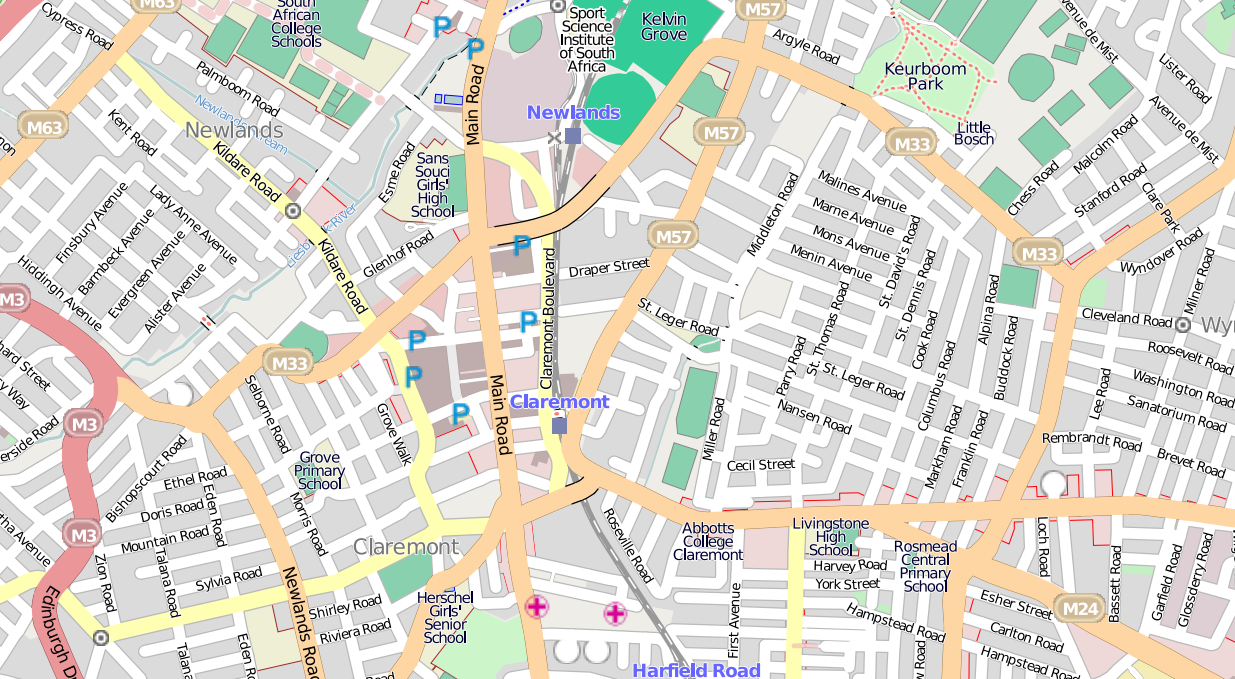
\includegraphics[width=0.9\linewidth]{context/maps}\\
		2D maps
	\end{minipage}%
	\pause%
	\begin{minipage}{0.5\linewidth}
		\centering
		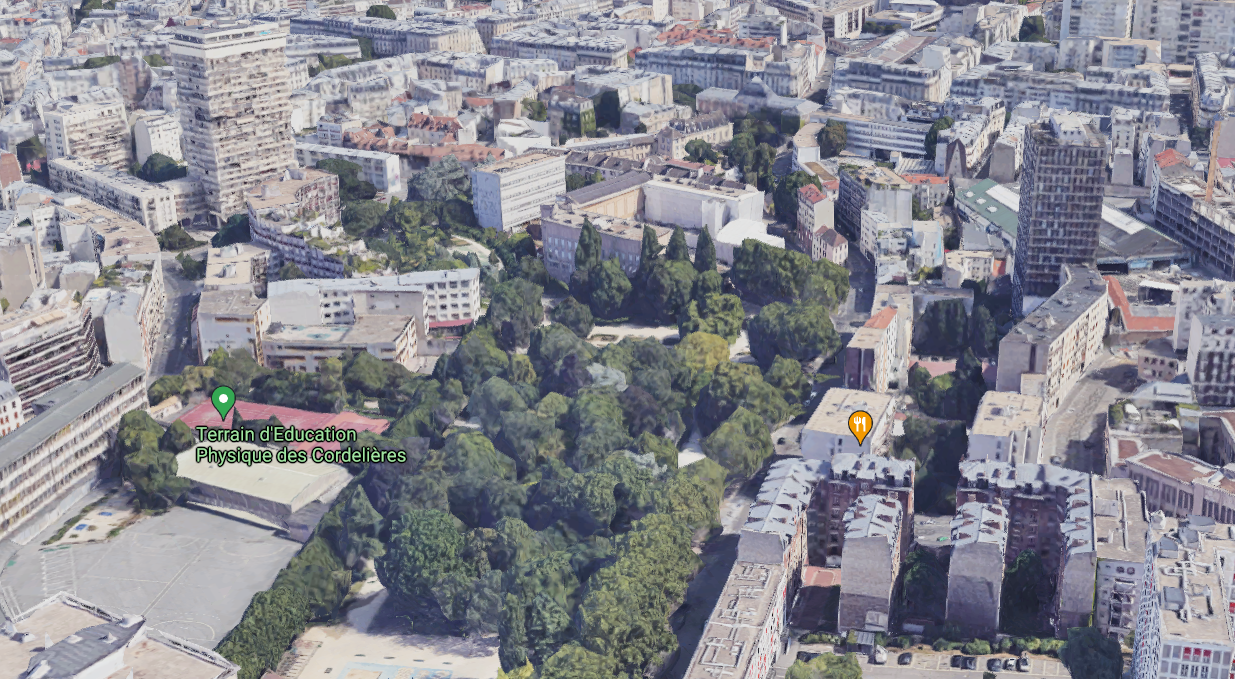
\includegraphics[width=0.9\linewidth]{context/dense_visu}\\
		3D visualization
	\end{minipage}%
	\pause
	
	\begin{minipage}{0.5\linewidth}
		\centering
		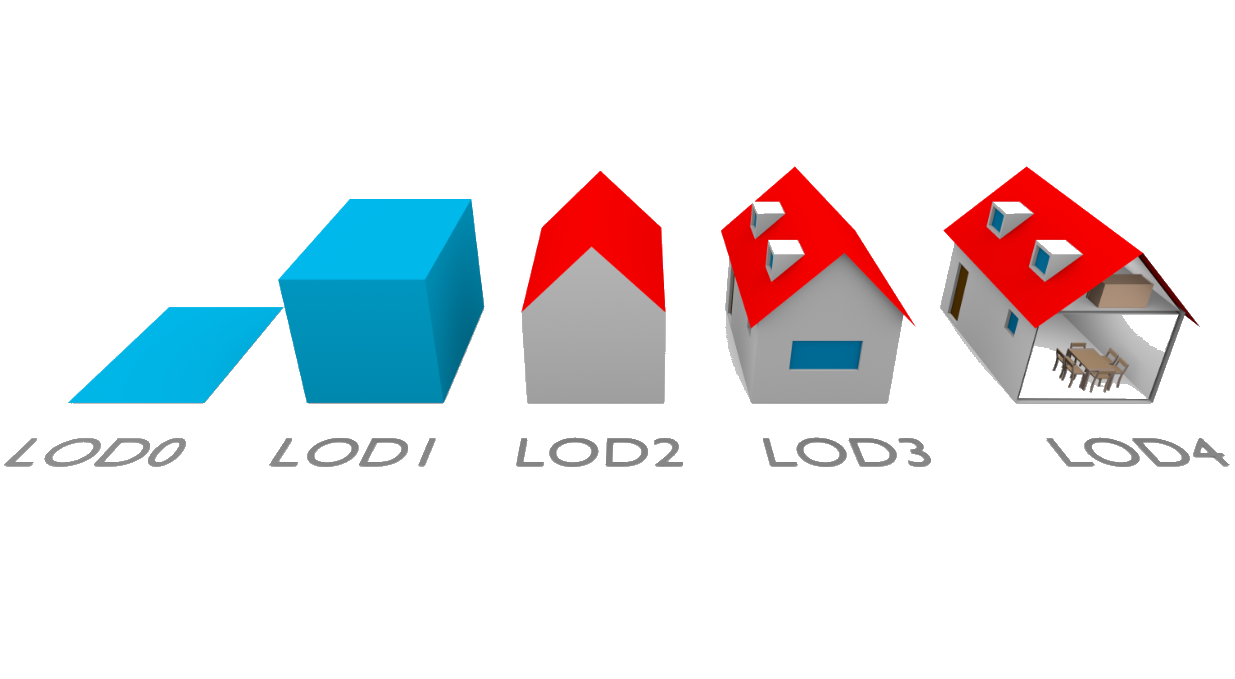
\includegraphics[width=0.9\linewidth]{context/lods}\\
		Geographic Information Systems (GIS)
	\end{minipage}%
	\pause%
	\begin{minipage}{0.5\linewidth}
		\centering
		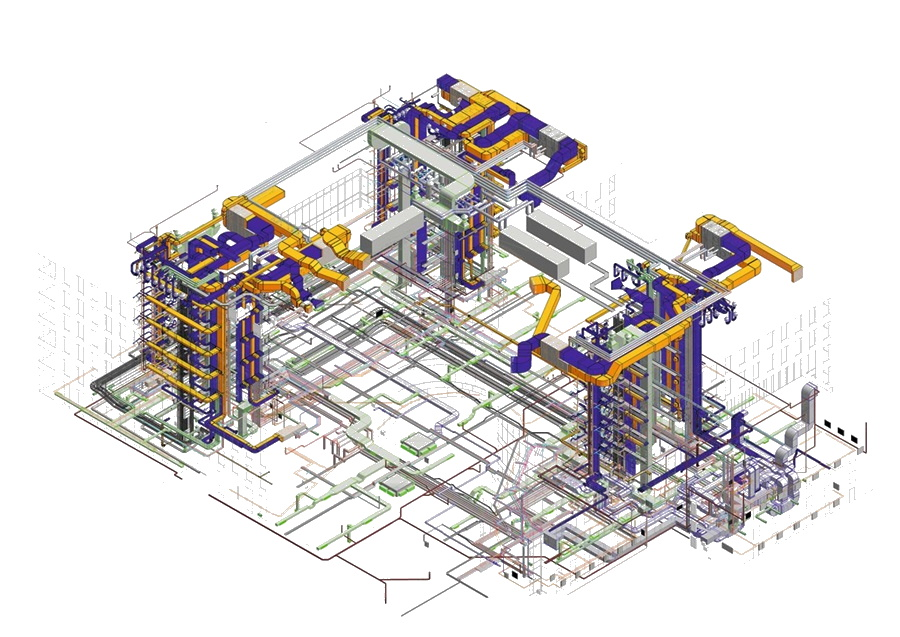
\includegraphics[width=0.9\linewidth]{context/bim}\\
		Building information model (BIM)
	\end{minipage}
\end{frame}

\begin{frame}[t]{Why do we need 3D models?}
	\textbf{Visualization}
	\vfill
	\begin{figure}
		\centering
		\begin{subfigure}[t]{0.45\linewidth}
			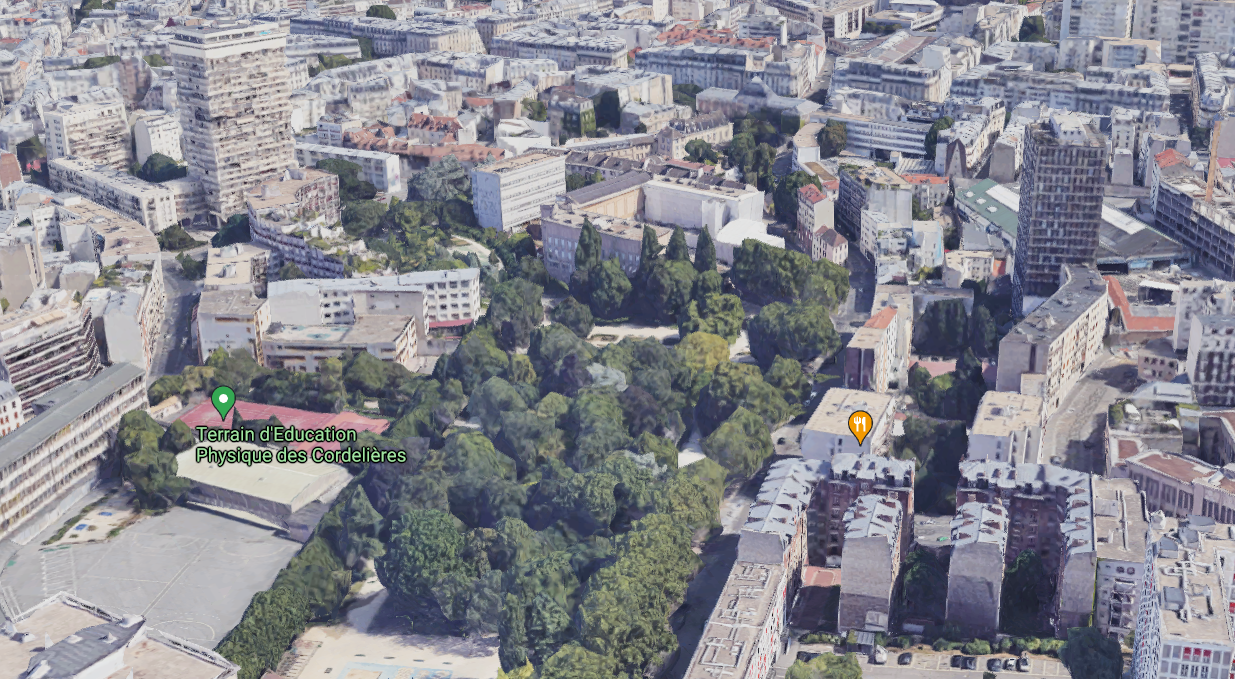
\includegraphics[width=\linewidth]{context/dense_visu}
			\subcaption*{Dense mesh representation \footnote[frame]{Google Maps}}
		\end{subfigure}
		\hfill%
		\begin{subfigure}[t]{0.45\linewidth}
			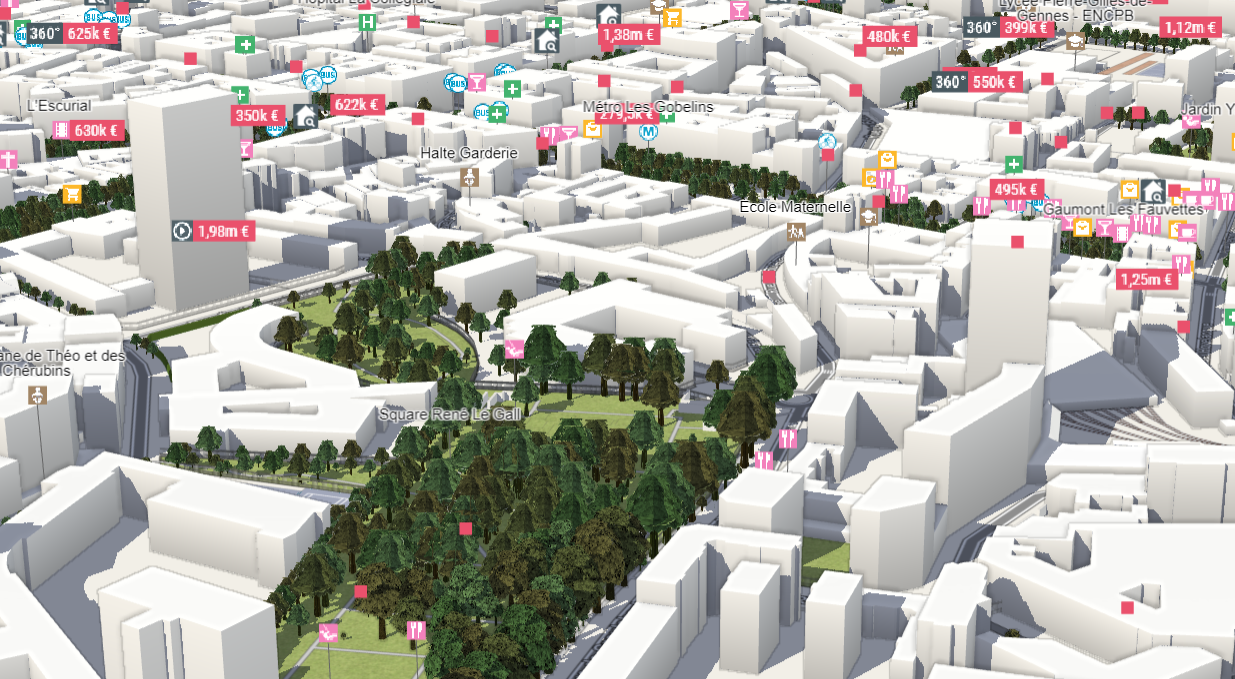
\includegraphics[width=\linewidth]{context/lod_visu}
			\subcaption*{LOD1 visualization \footnote[frame]{Bien'ici}}
		\end{subfigure}
	\end{figure}
\end{frame}

\begin{frame}[t]{Why do we need 3D models?}
	\textbf{Simulation}
	\vfill
	\begin{figure}
		\centering
		\begin{subfigure}[t]{0.45\linewidth}
			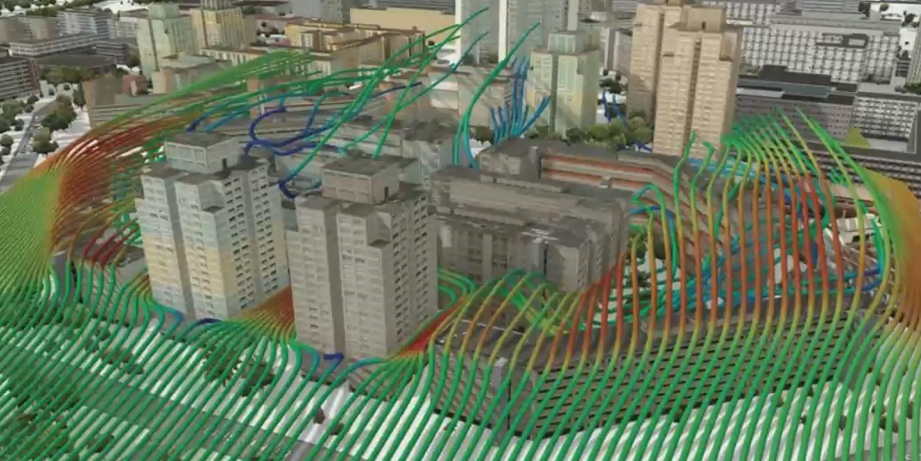
\includegraphics[width=\linewidth]{context/simulation_wind}
			\subcaption*{Wind simulation \footnote[frame]{SIMULIA, Dassault Systèmes}}
		\end{subfigure}
		\hfill%
		\begin{subfigure}[t]{0.45\linewidth}
			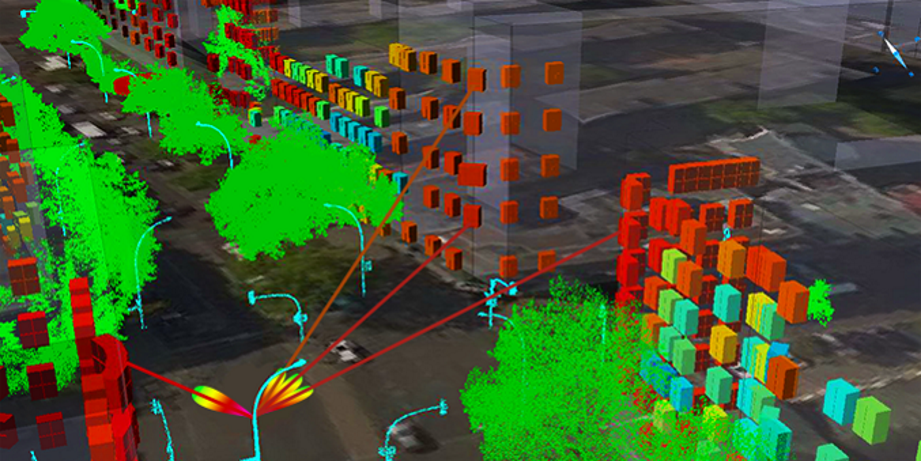
\includegraphics[width=\linewidth]{context/simulation_lineofsight}
			\subcaption*{5G connectivity \footnote[frame]{SIRADEL}}
		\end{subfigure}
	\end{figure}
\end{frame}

\begin{frame}[t]{Why do we need 3D models?}
	\textbf{Change tracking}
	\vfill
	\begin{figure}
		\centering
		\begin{subfigure}[t]{0.45\linewidth}
			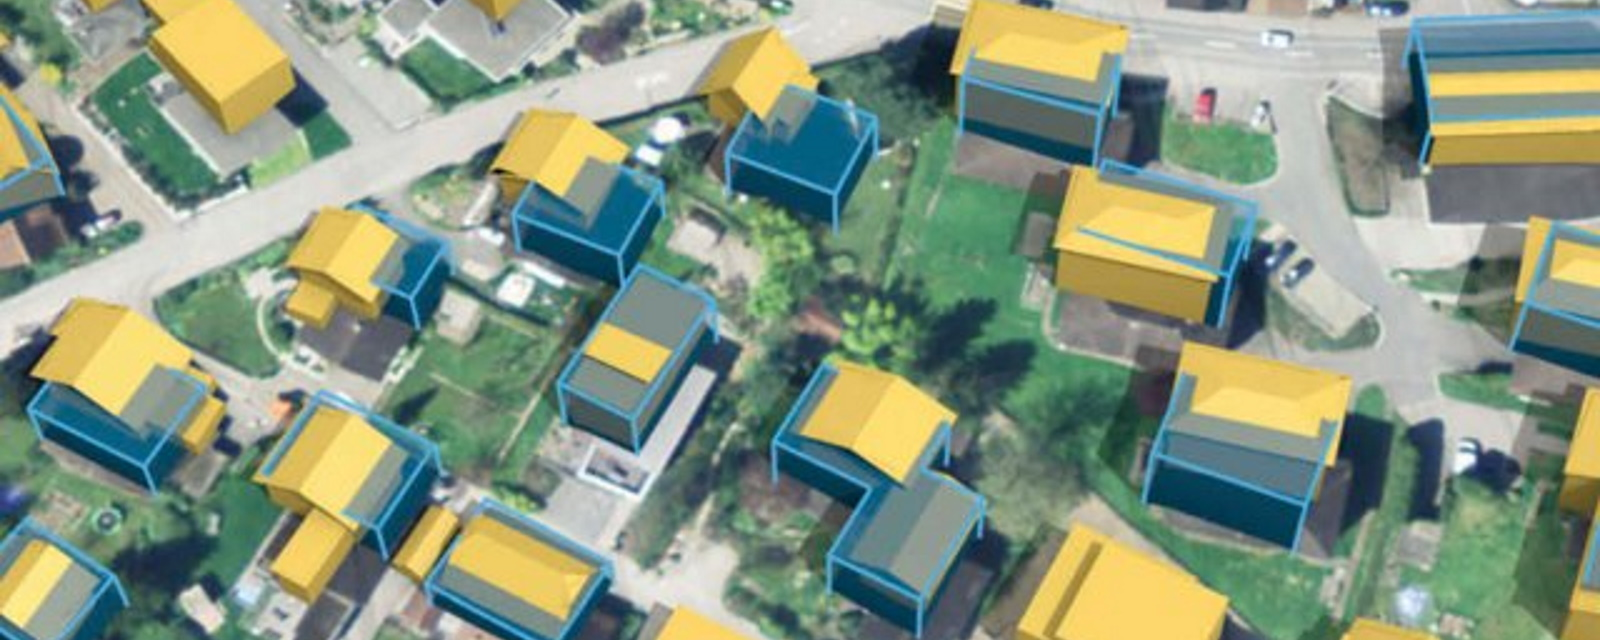
\includegraphics[width=\linewidth]{context/lod_diff_v2}
			\subcaption*{Permit verification \footnote[frame]{Taken from \cite{biljecki_EffectAcquisition_2018}}}
		\end{subfigure}%
		\hfill%
		\begin{subfigure}[t]{0.45\linewidth}
			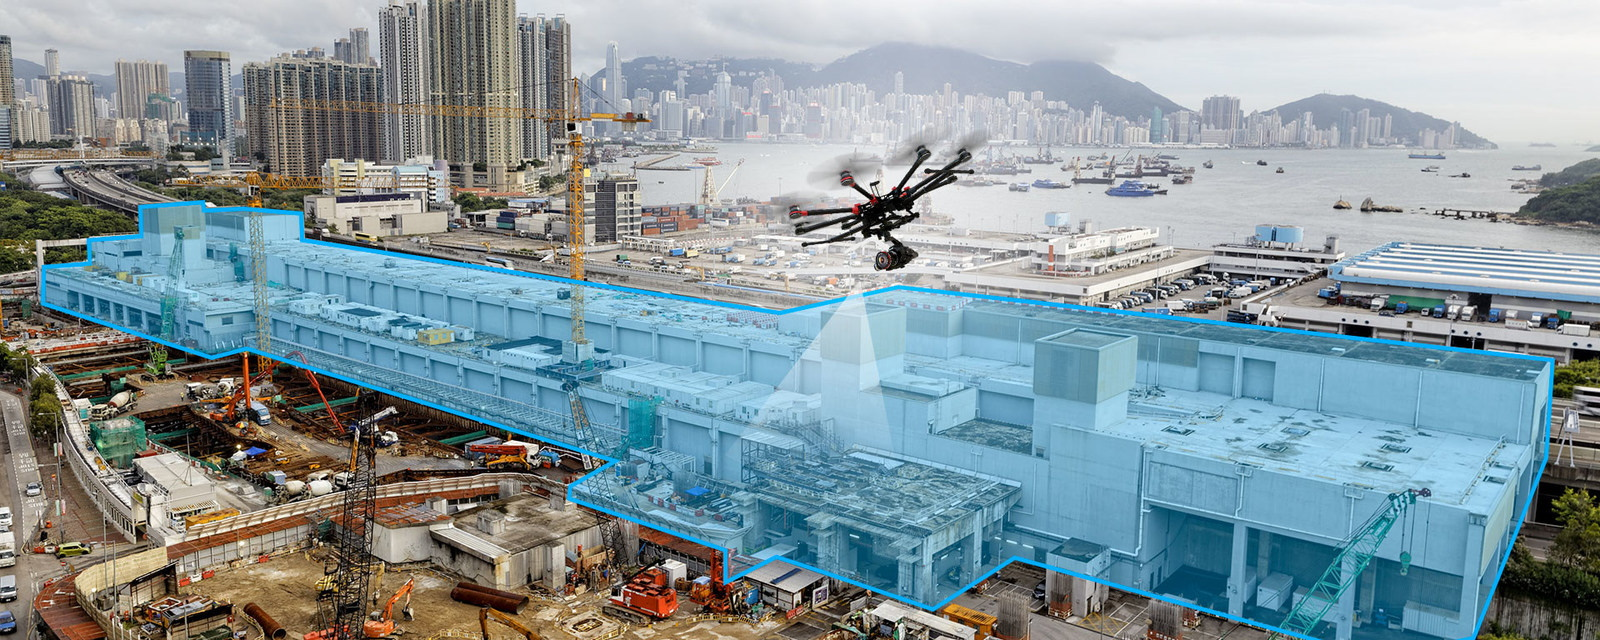
\includegraphics[width=\linewidth]{context/building_inspection}
			\subcaption*{Building inspection \footnote[frame]{\href{https://www.engineering.com/story/automating-facility-inspection-with-drones}{Engineering.com \ExternalLink}}}
		\end{subfigure}
	\end{figure}	
\end{frame}

\begin{frame}{Acquisitions}
	\small
	\centering
	\begin{minipage}{0.5\linewidth}
		\centering
		\textbf{LiDAR technologies}
	\end{minipage}%
	\begin{minipage}{0.5\linewidth}
		\centering
		\textbf{Photogrammetry}
	\end{minipage}

	\begin{minipage}{0.5\linewidth}
		\centering
		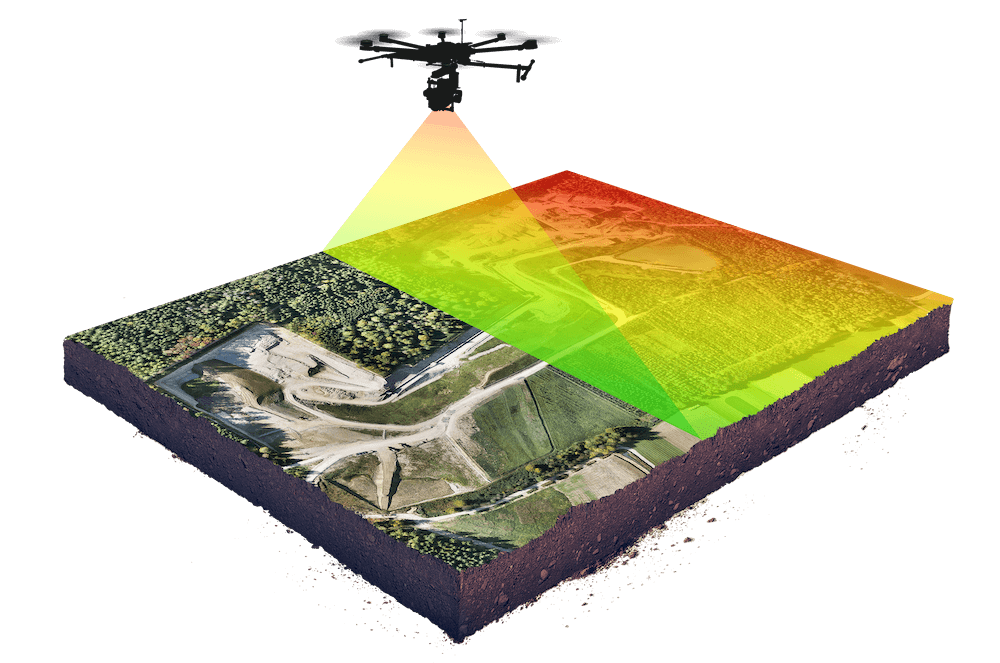
\includegraphics[width=0.7\linewidth]{context/lidar_method}			
	\end{minipage}%
	\begin{minipage}{0.5\linewidth}
		\centering
		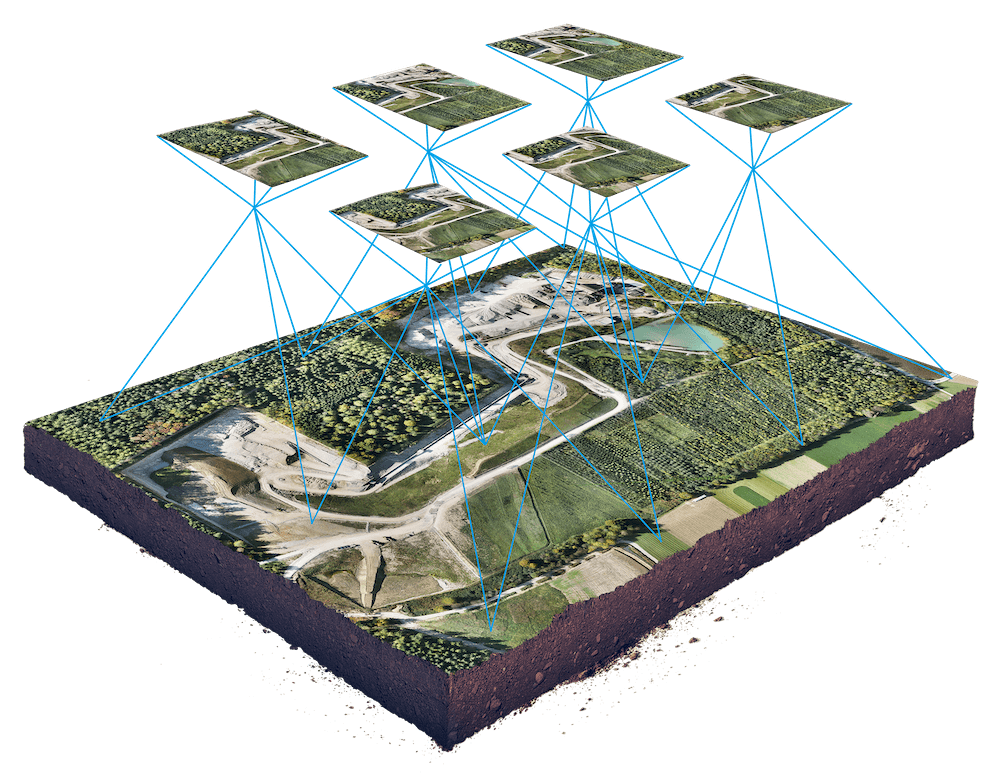
\includegraphics[width=0.7\linewidth]{context/photo_method}
	\end{minipage}

	\begin{minipage}{0.5\linewidth}
		\centering
		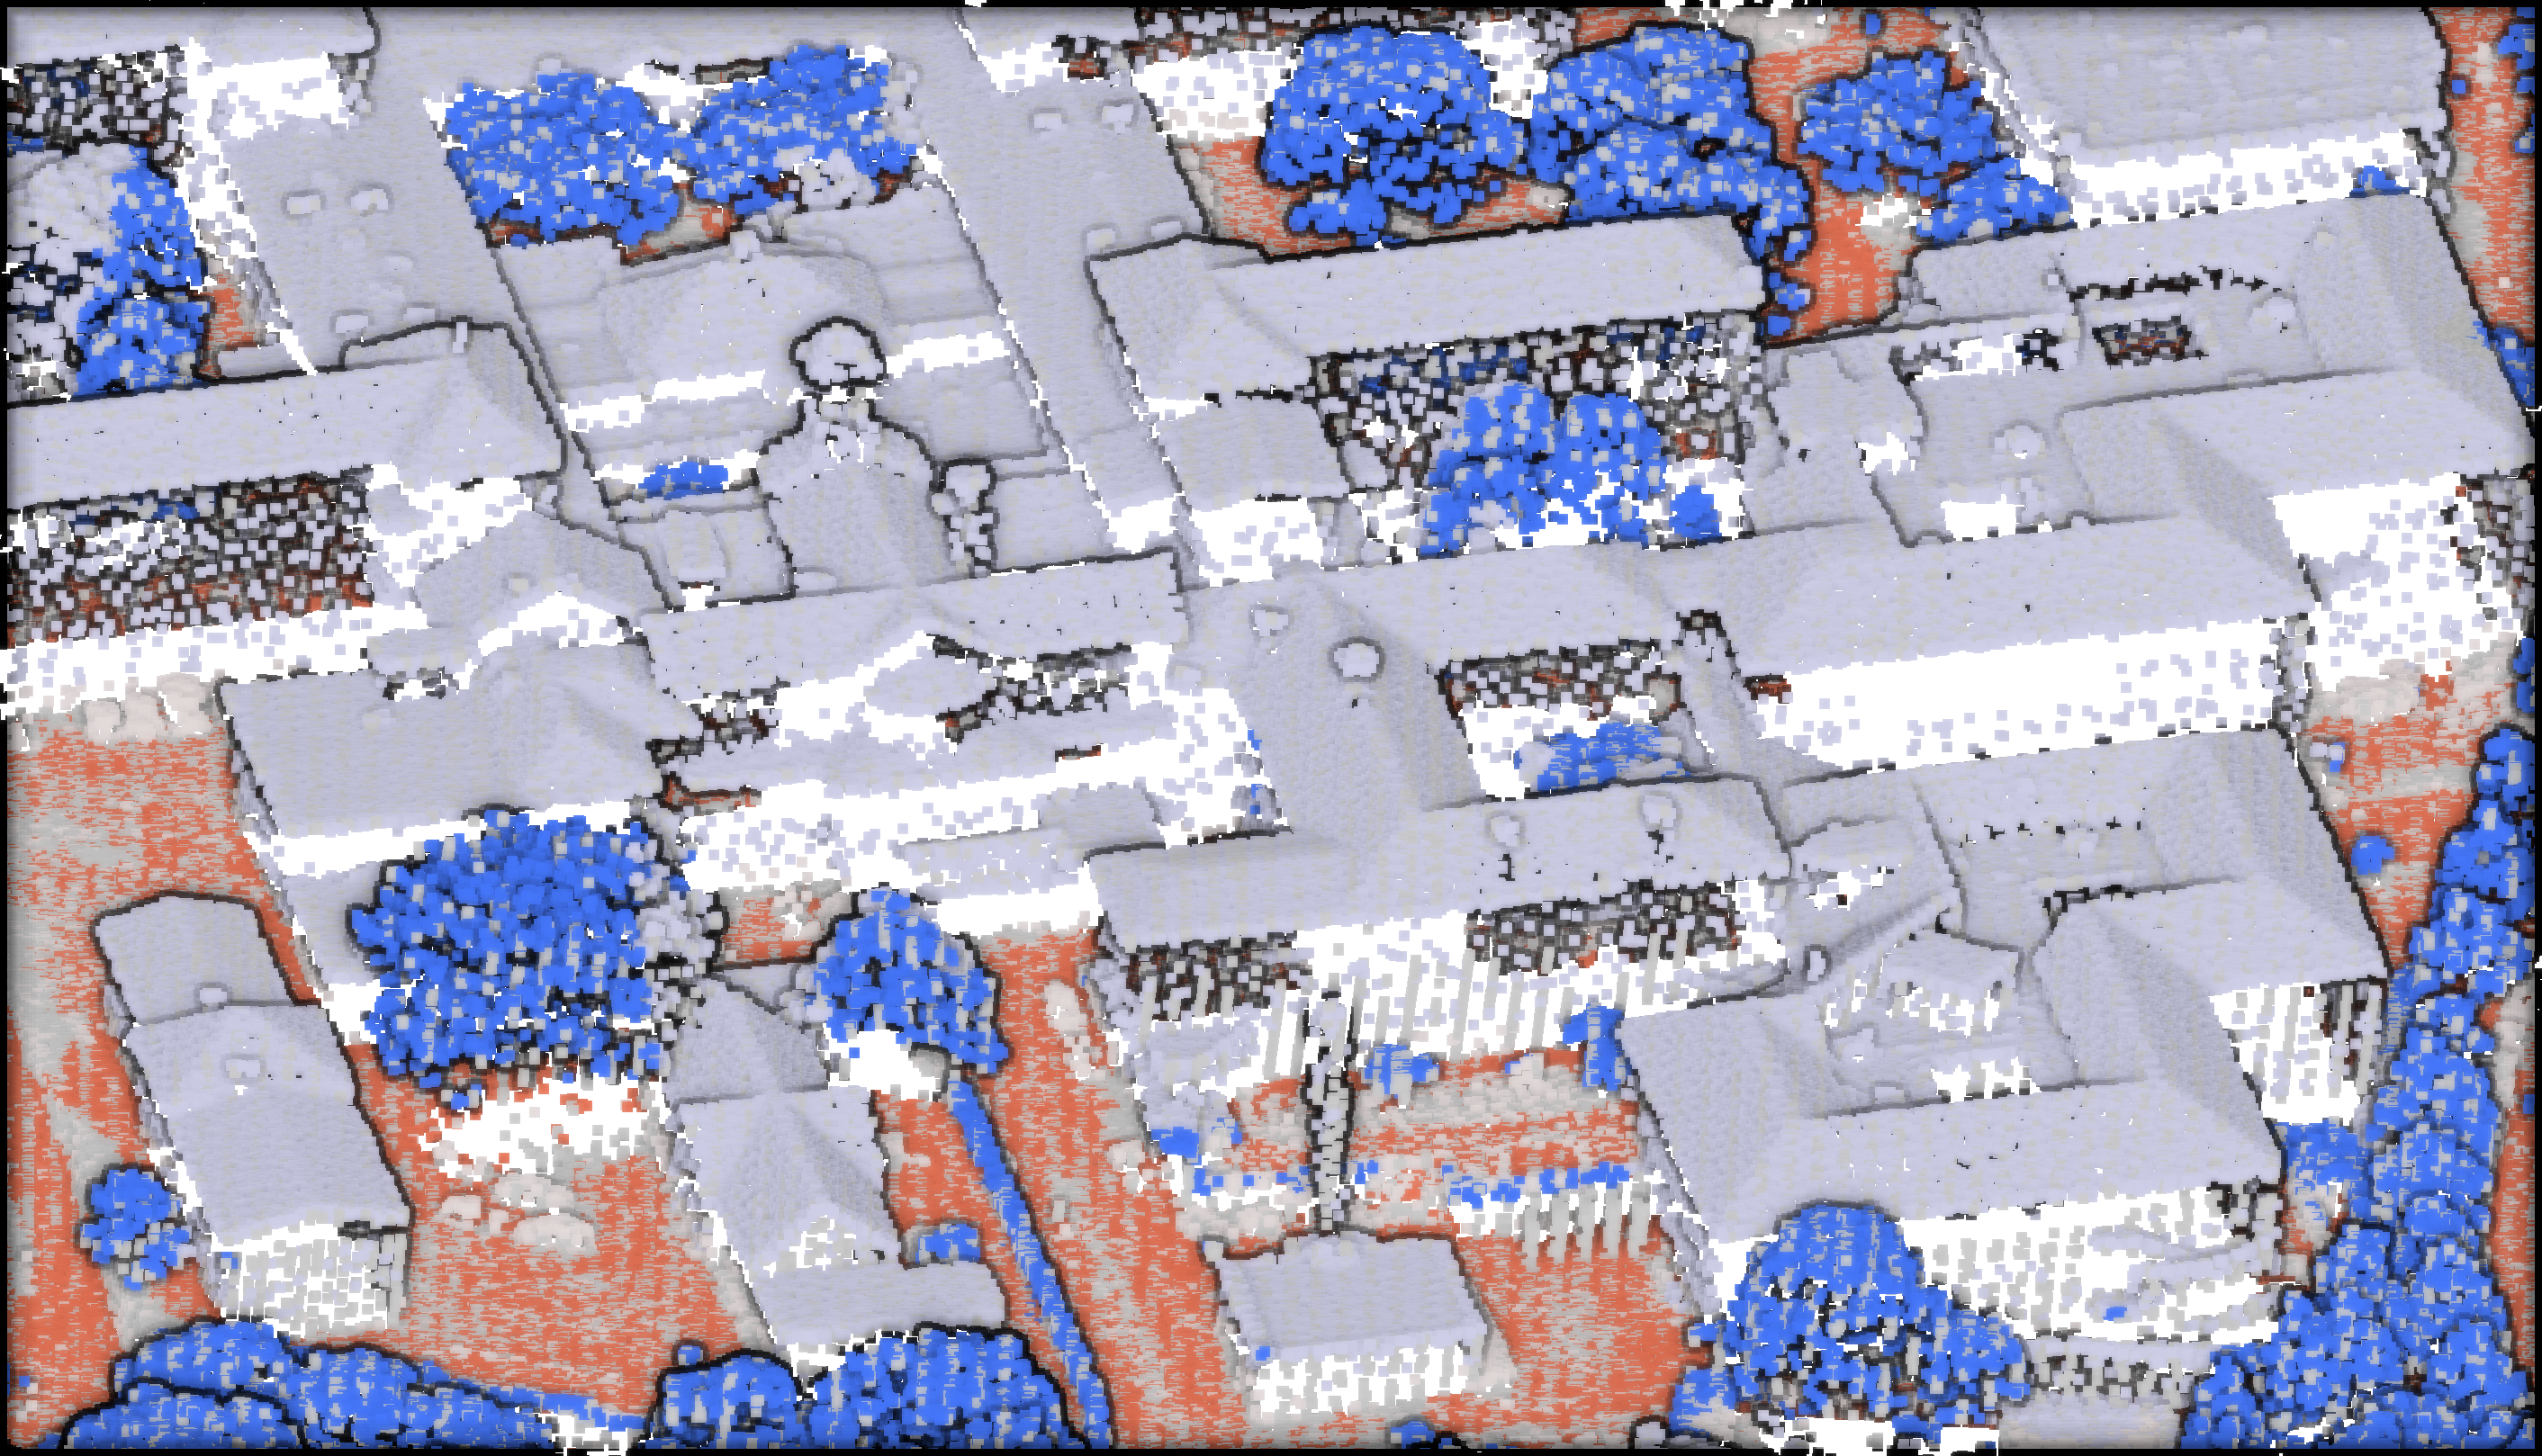
\includegraphics[width=0.8\linewidth]{context/lidar}	
	\end{minipage}%
	\begin{minipage}{0.5\linewidth}
		\centering
		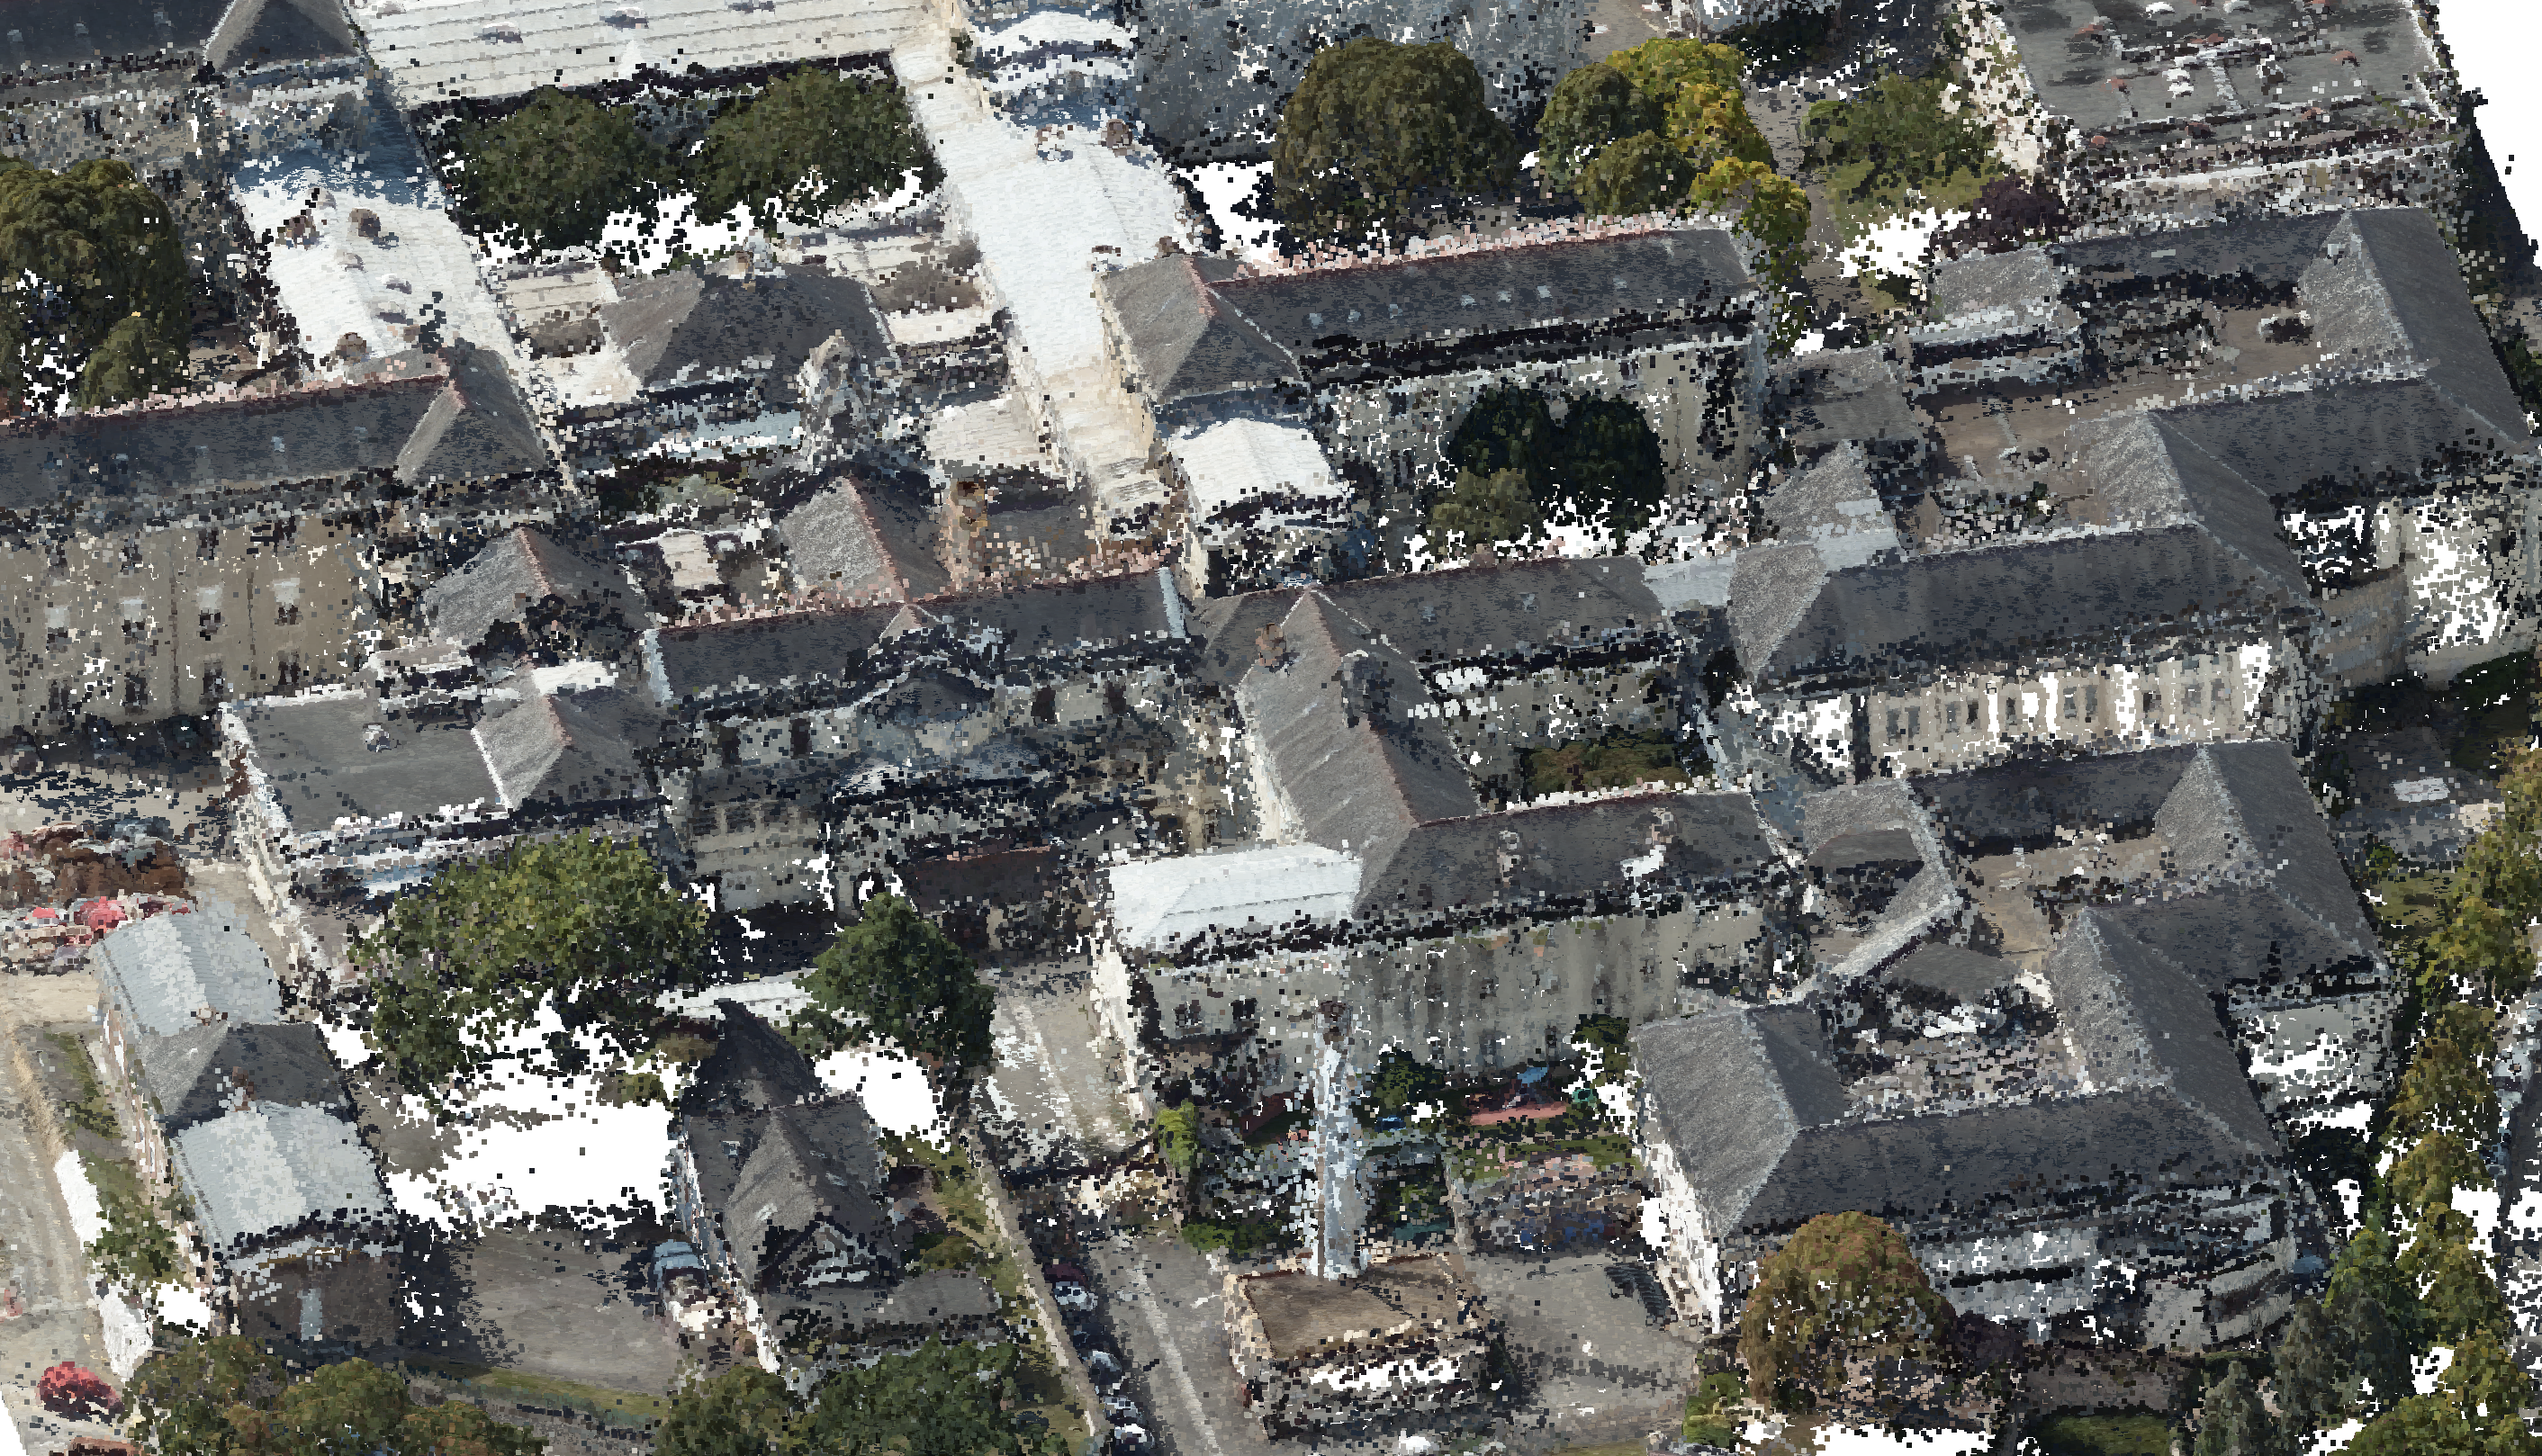
\includegraphics[width=0.8\linewidth]{context/photogrammetry}	
	\end{minipage}%
	
	\blfootnote{Images from \href{https://wingtra.com/drone-photogrammetry-vs-lidar}{Wingtra \ExternalLink}}
\end{frame}

\begin{frame}{Scope of interest}
	\textbf{Inputs:} Point clouds (LiDAR or Photogrammetry) \\
	\textbf{Semi-automatic} methods \\
	\pause
	
	\vspace{0.5cm}
	
	\begin{tabular}{ll}
		\textbf{Parsimonious representation} & \textbf{Dense representation} \\
		LOD2 reconstruction & Triangular mesh \\
		Buildings & Any urban object \\
		Strong regularity priors & No priors \\
	\end{tabular}
\end{frame}
	\graphicspath{{images/arrangements/}}

\section{Parsimonious representations from 2D partitions}

%\begin{frame}{Approaches}
%	
%\begin{frame}
	
\begin{frame}{Reconstruction pipeline}
	\begin{minipage}[b]{0.2\linewidth}
	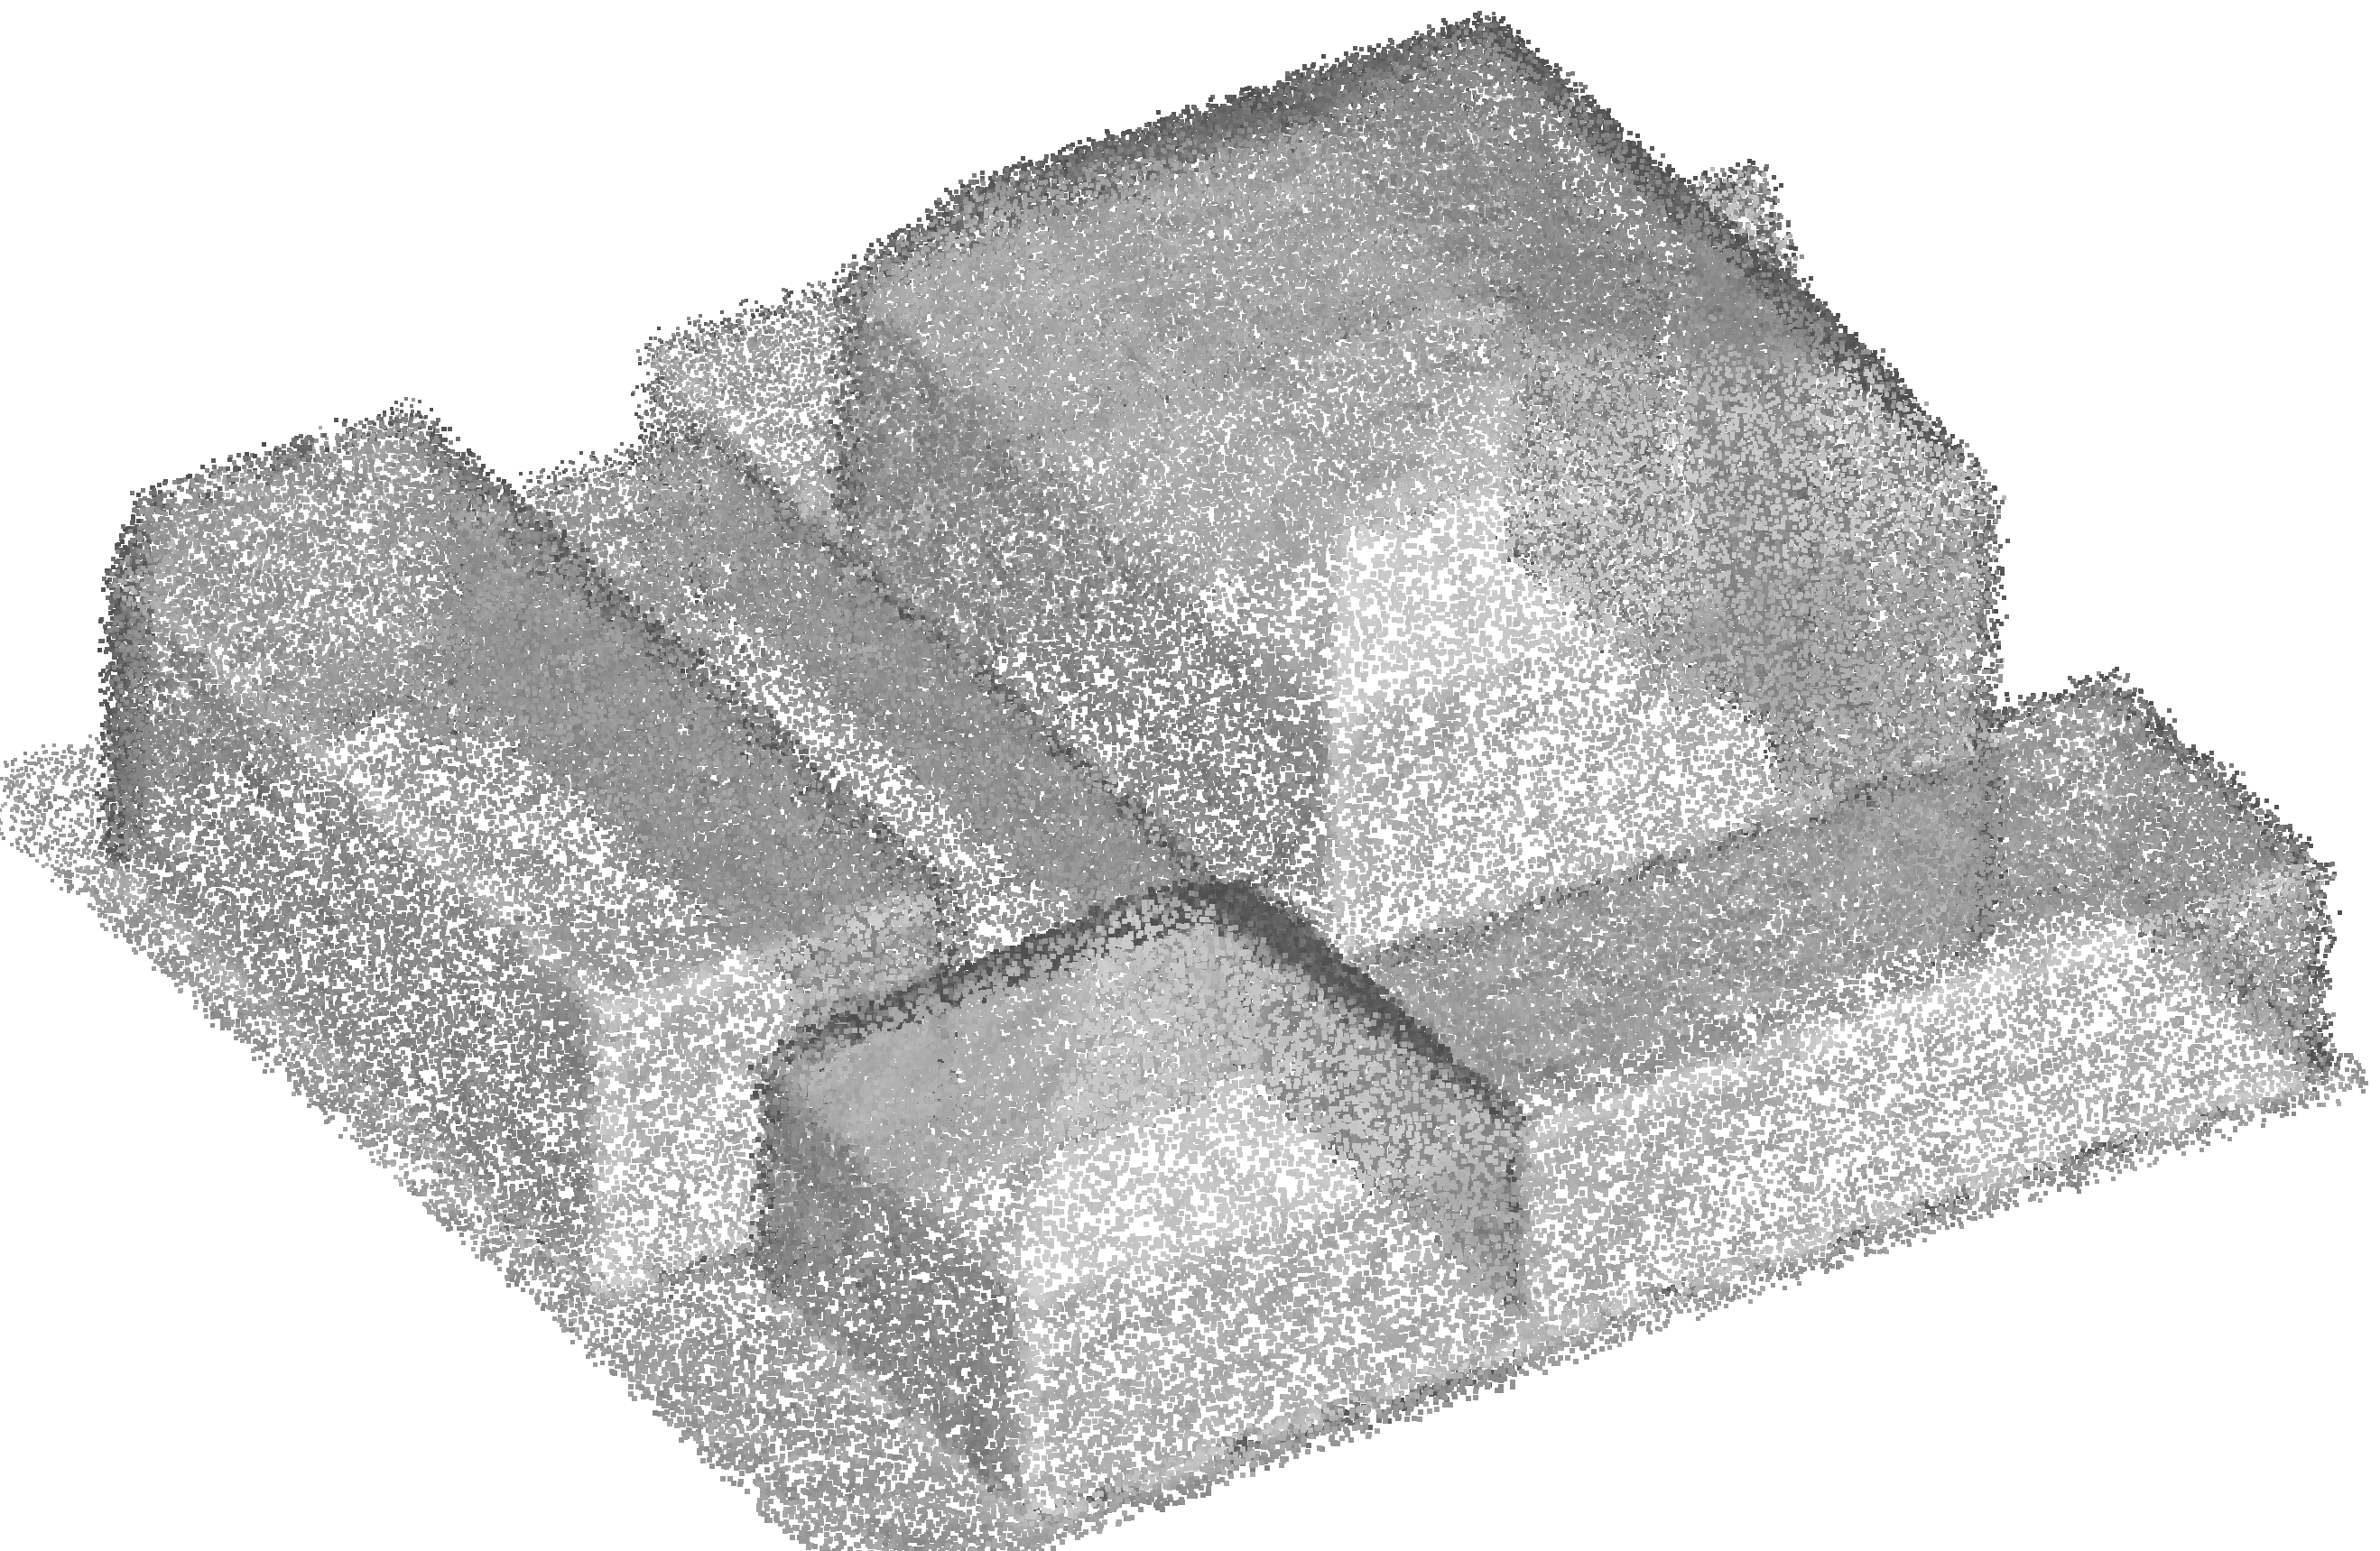
\includegraphics[width=\linewidth]{pipeline/pointcloud_crop}
	\end{minipage}%
	\begin{minipage}[b]{0.2\linewidth}
		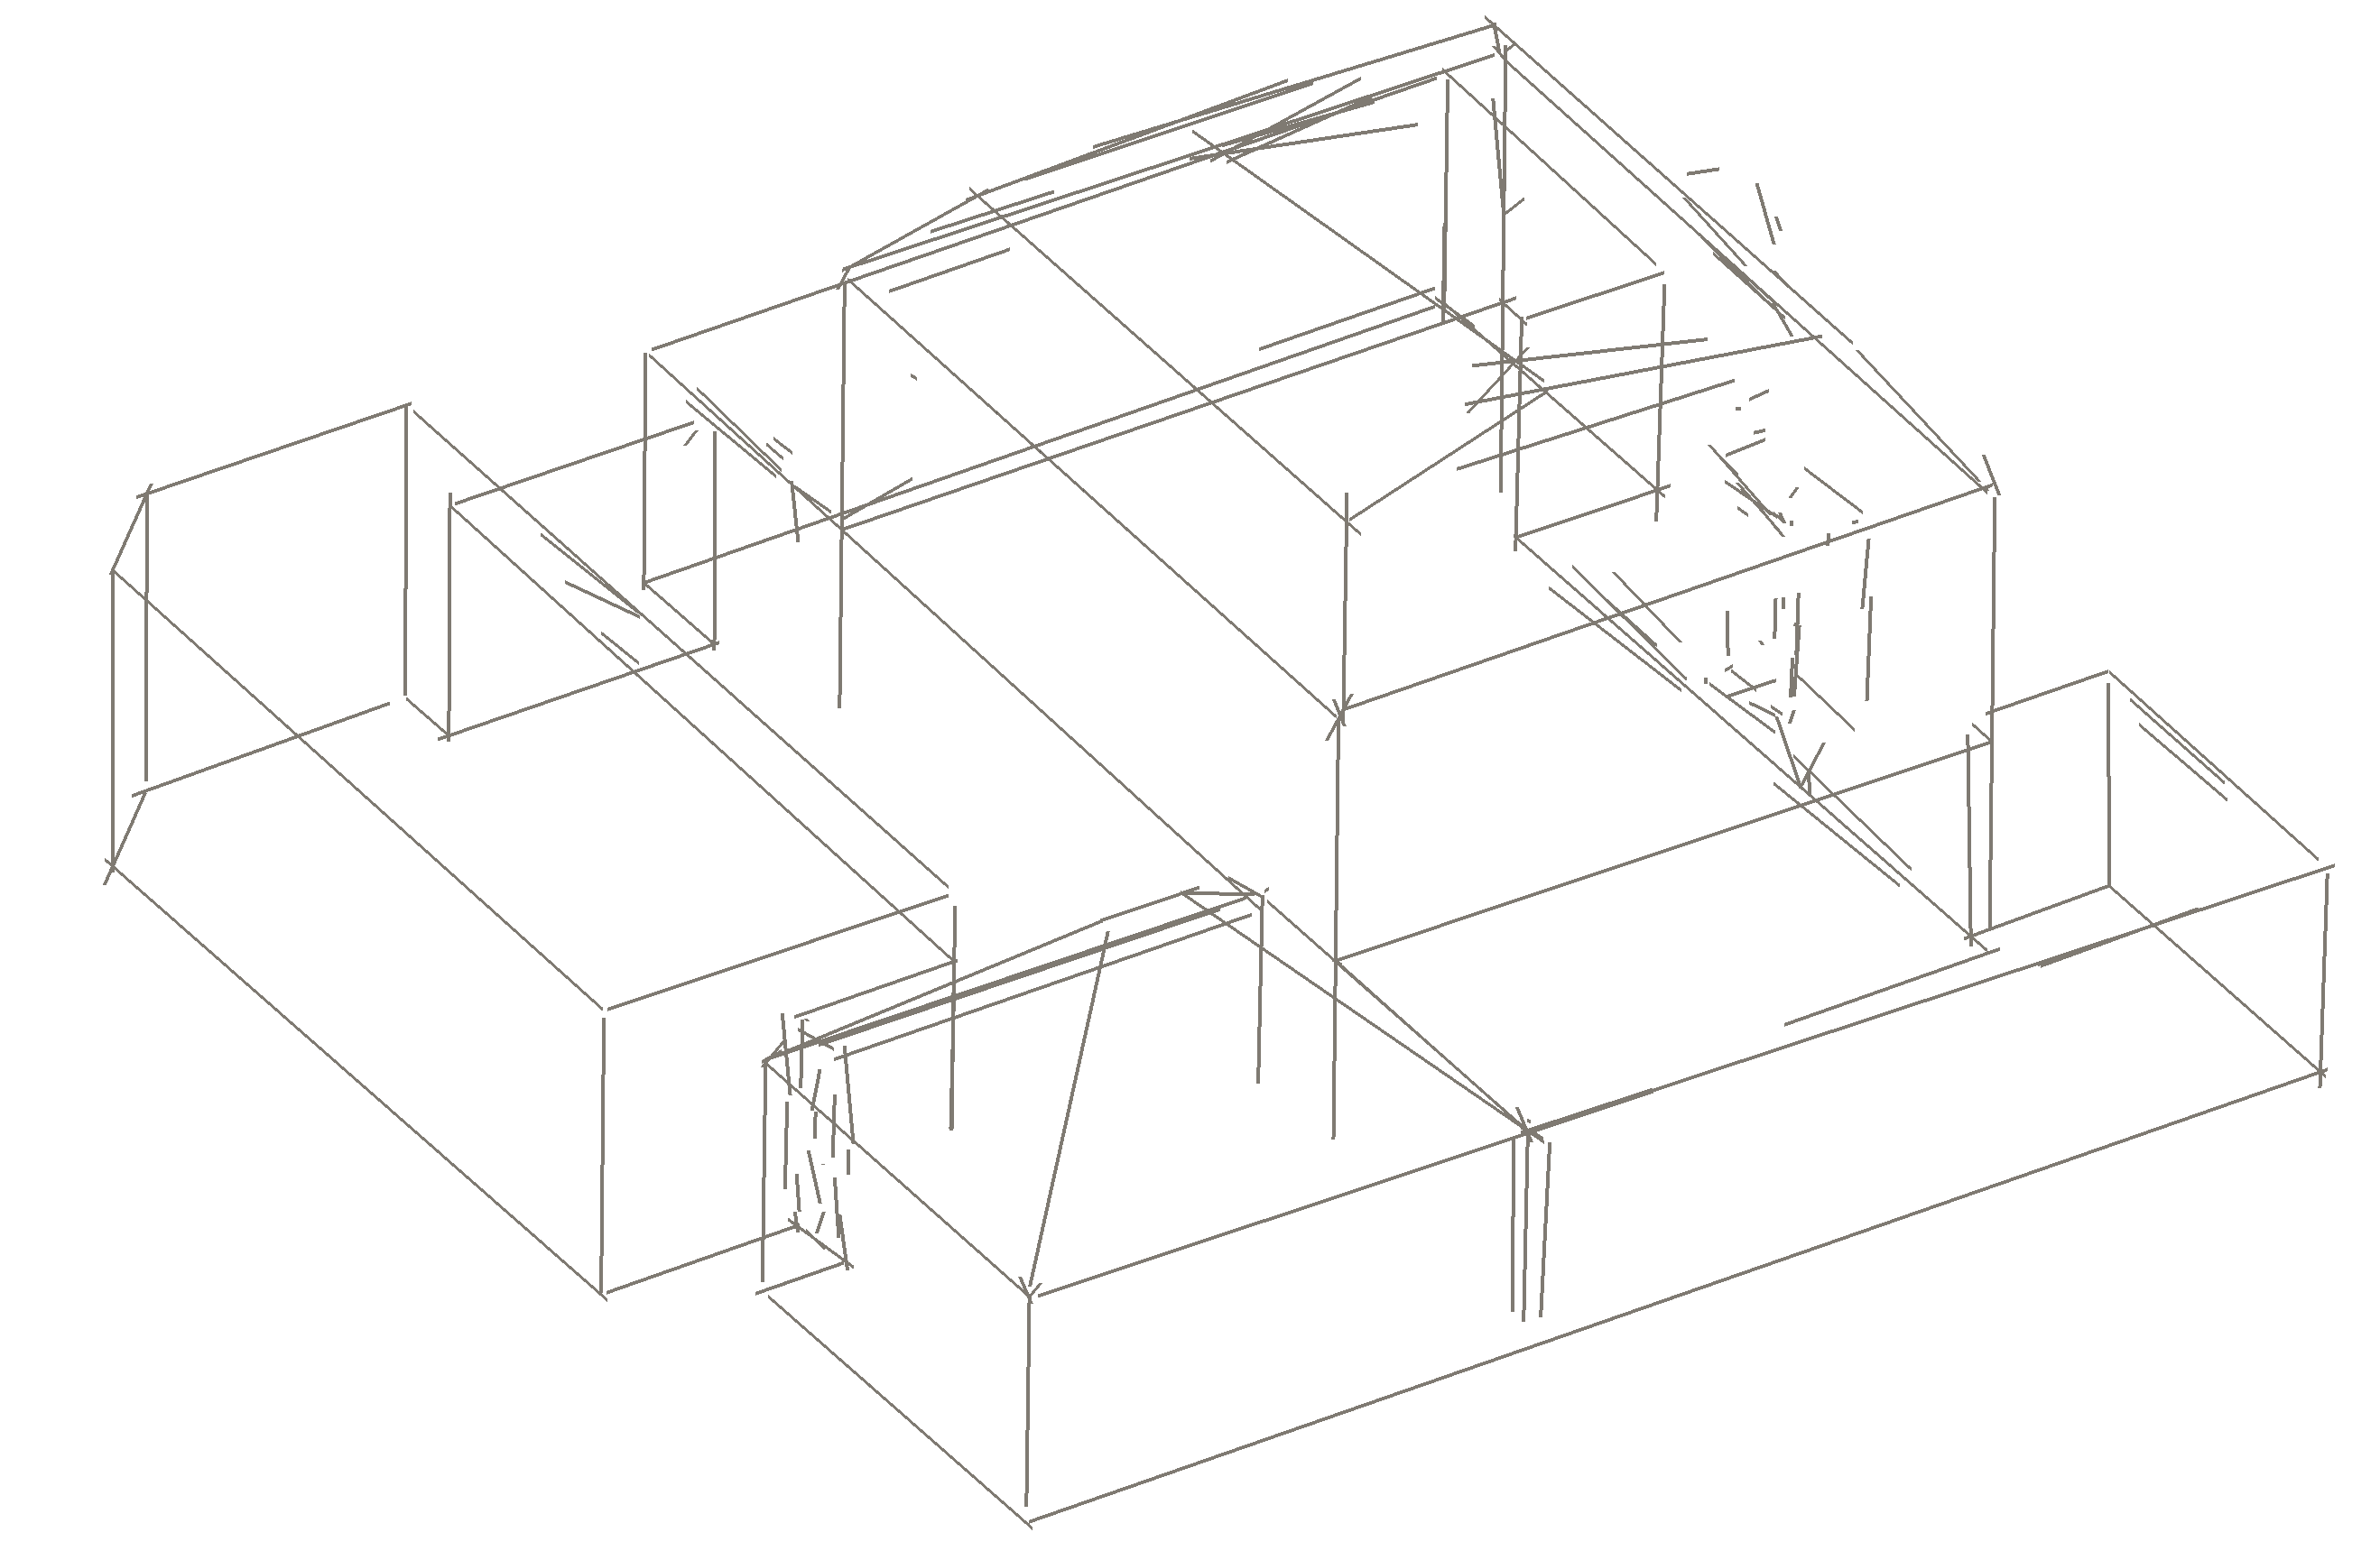
\includegraphics[width=\linewidth]{pipeline/segments_crop}
	\end{minipage}%
	\begin{minipage}[b]{0.2\linewidth}
		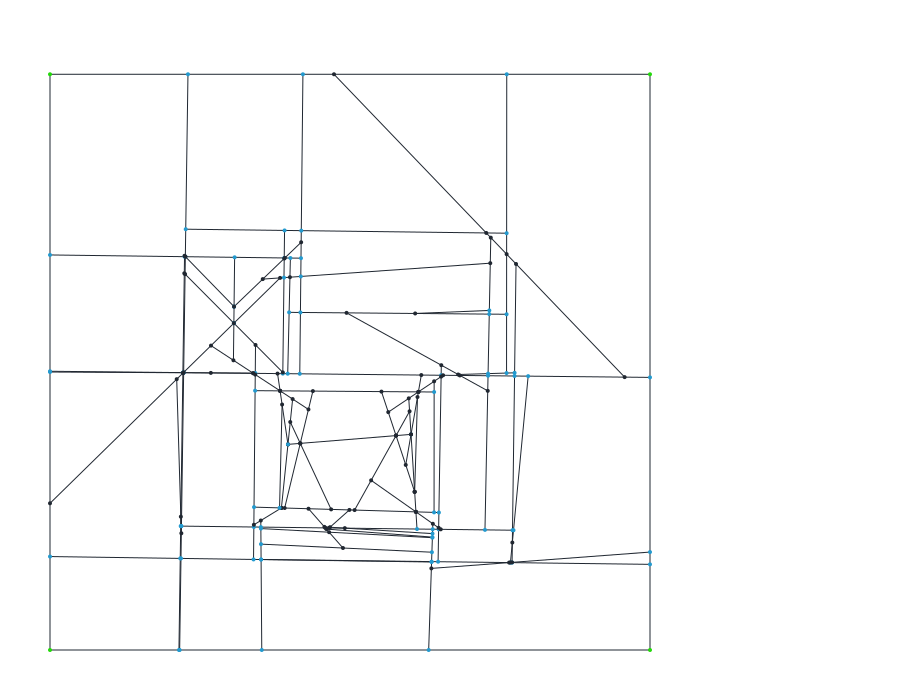
\includegraphics[width=\linewidth]{pipeline/original}
	\end{minipage}%
	\begin{minipage}[b]{0.2\linewidth}
		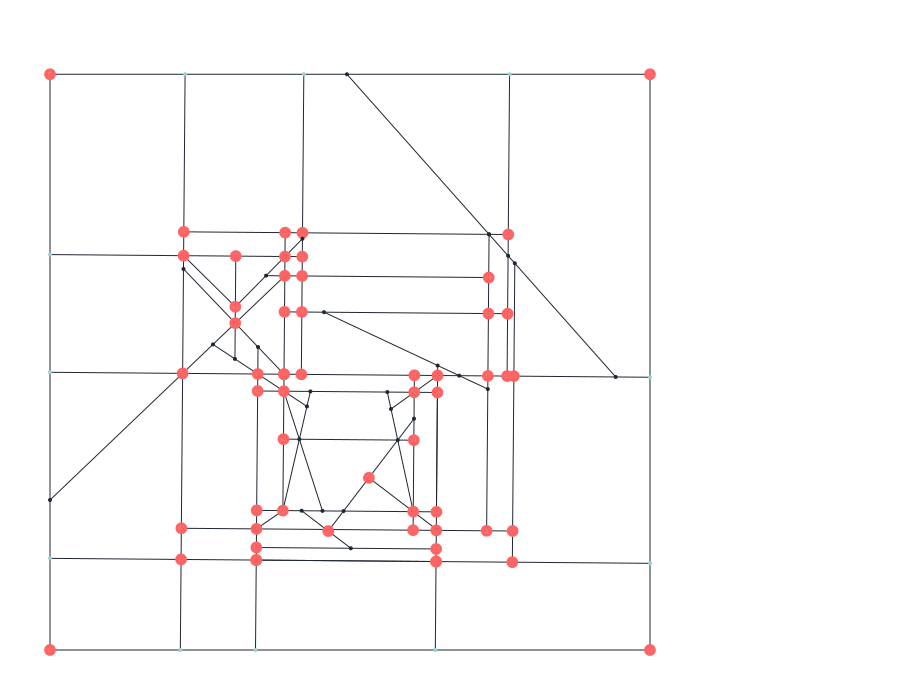
\includegraphics[width=\linewidth]{pipeline/simplified}
	\end{minipage}%
	\begin{minipage}[b]{0.2\linewidth}
		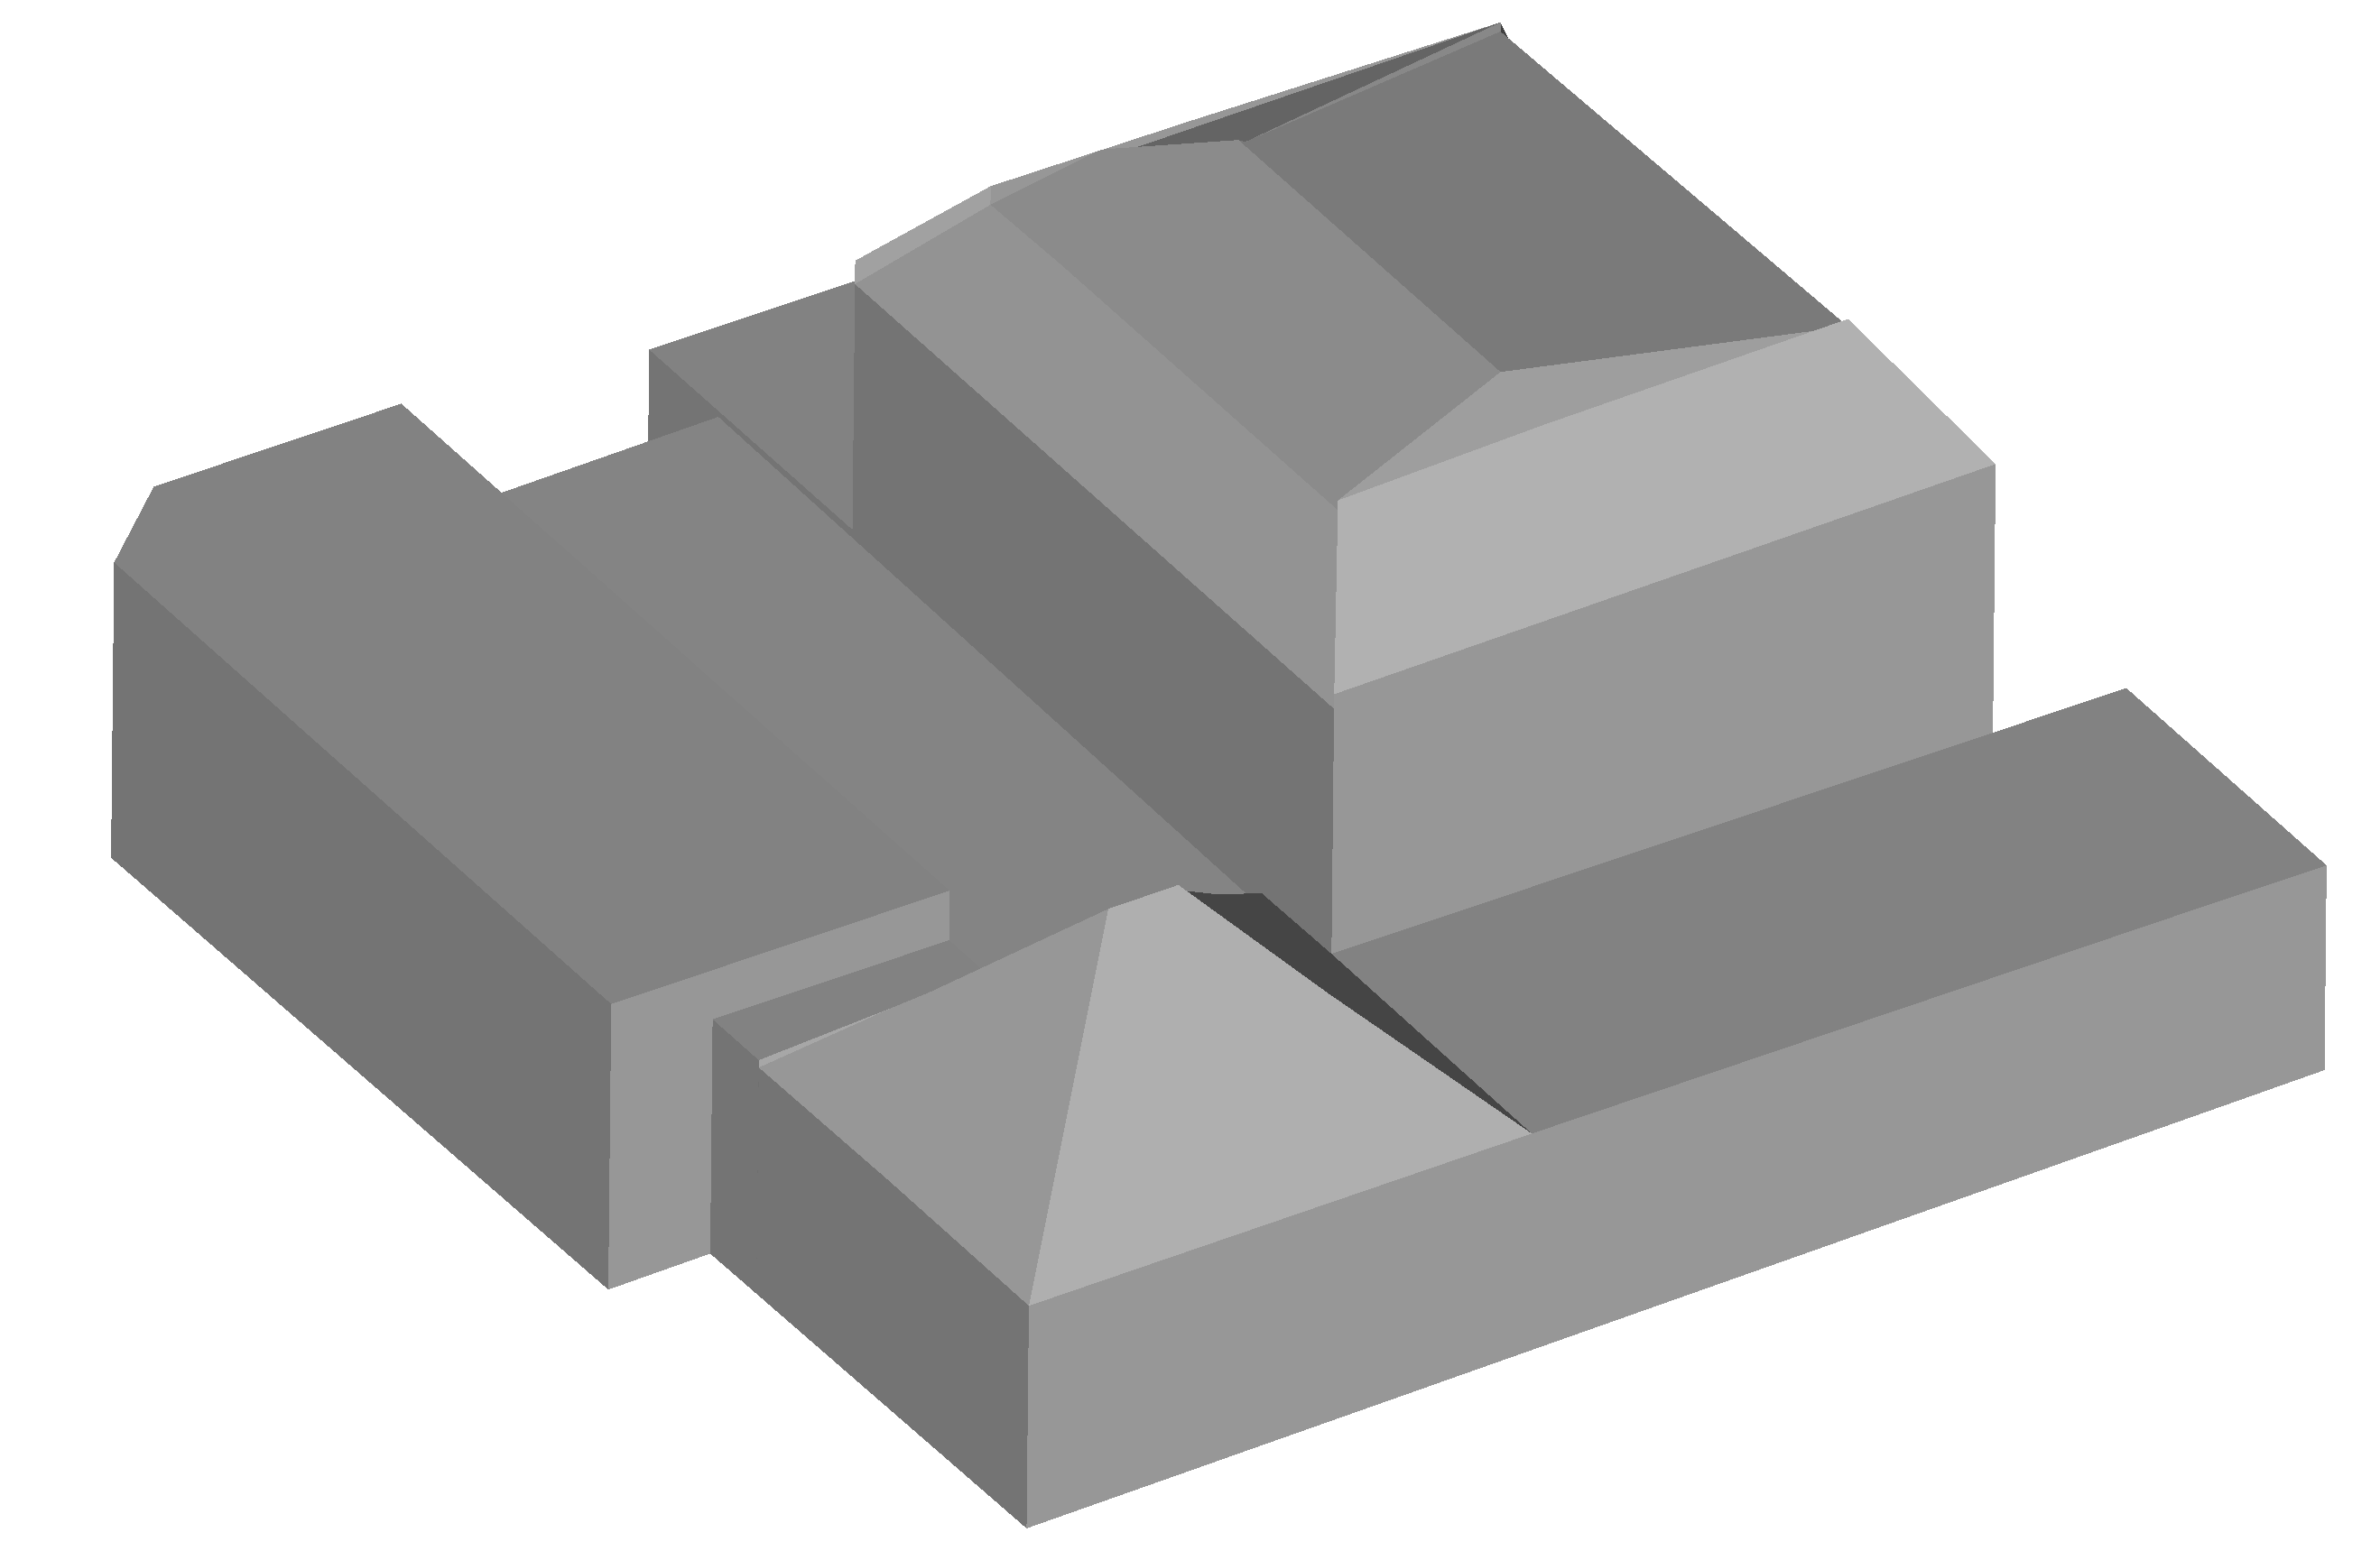
\includegraphics[width=\linewidth]{pipeline/mesh_crop}
	\end{minipage}

	\begin{itemize}
		\item Input: Point clouds, Photogrammetry or Structure-from-Motion (SfM)
		\item Segment detection
		\item Kinetic partition
		\item Simplification
		\item Lifted model (LOD2 representation for GIS)
	\end{itemize}
\end{frame}

\begin{frame}{Segment detection}
	\begin{center}
		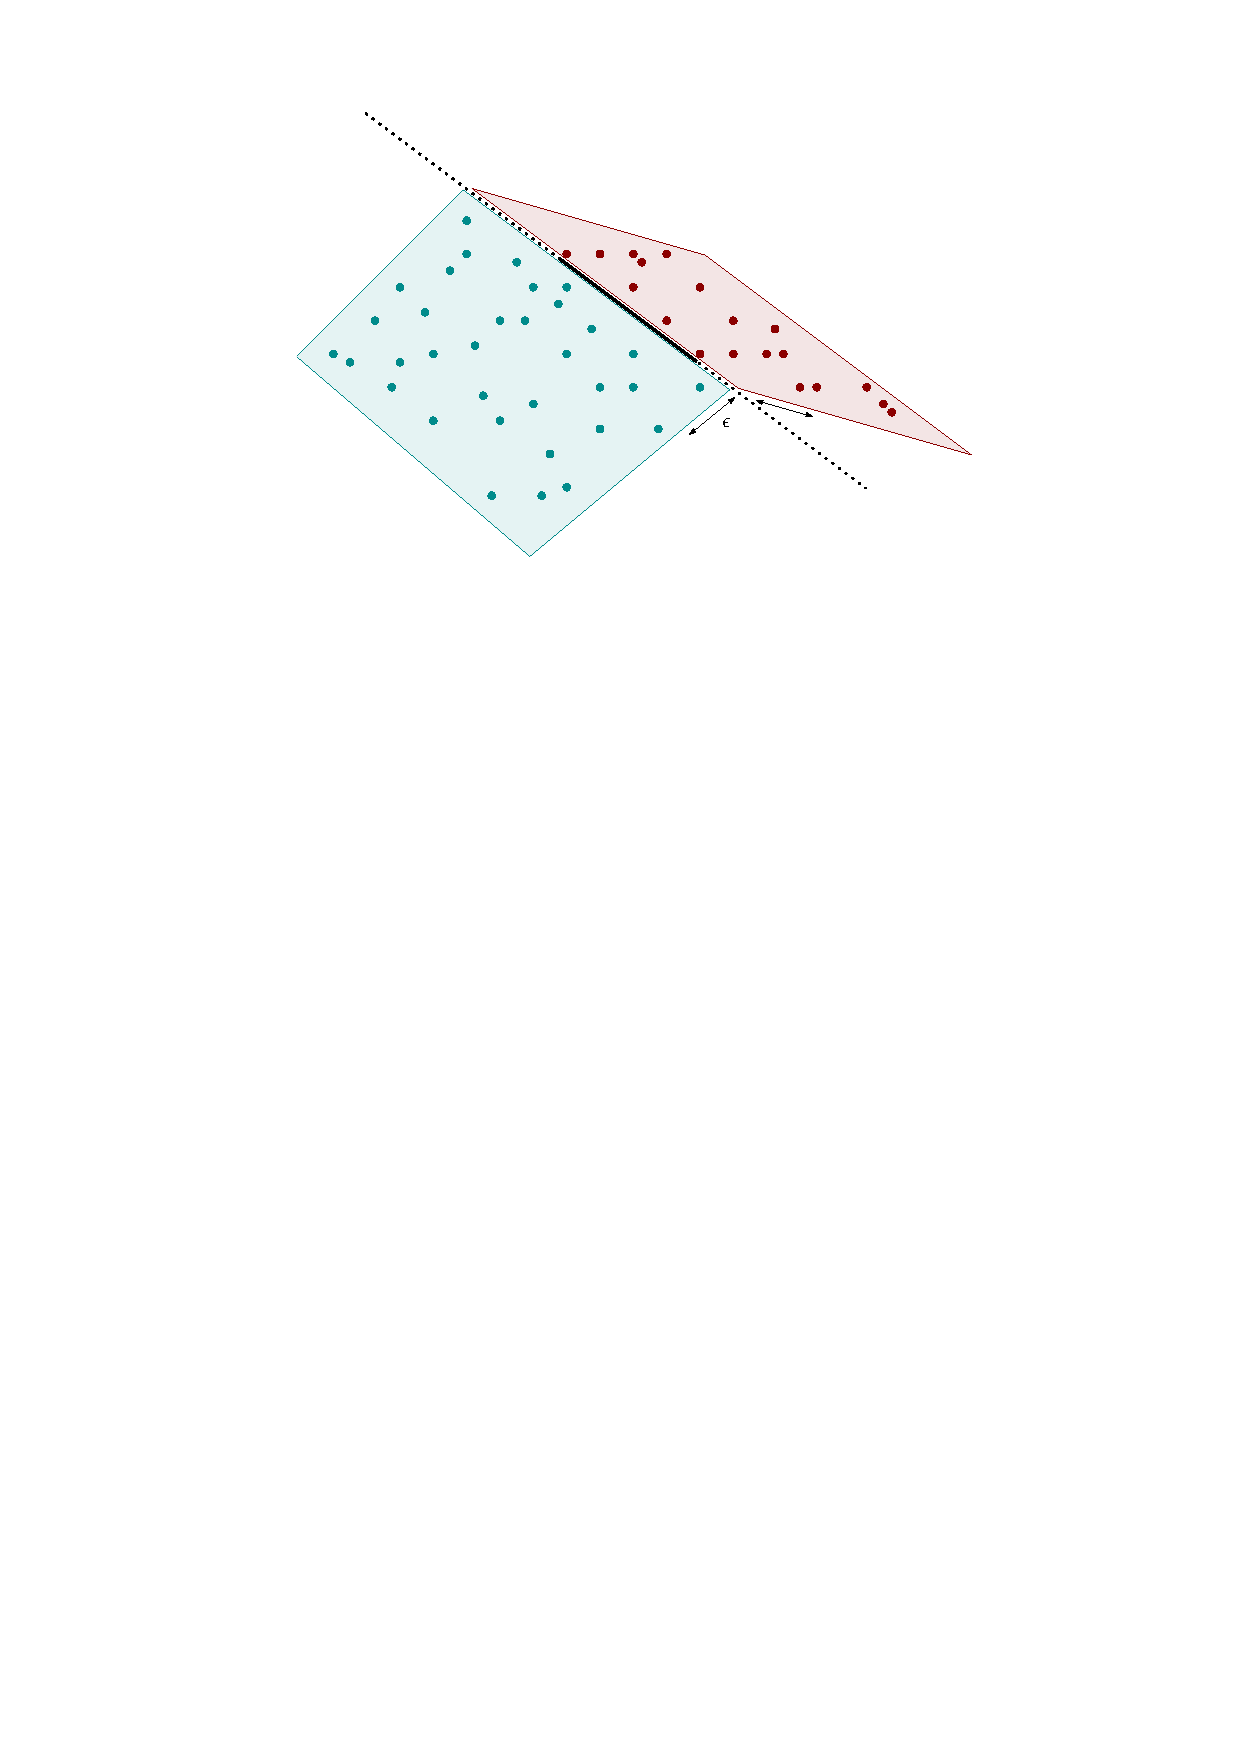
\includegraphics[width=0.5\textwidth]{plane_detection}
	\end{center}
	\textbf{Plane detection} using $k$-NN and region-growing \cite{feng_FastPlaneExtraction_2014, holz_FastRangeImage_2013, rabbani_SegmentationPointClouds_2006}.\\
	\textbf{Intersection lines} from adjacent planar primitives.\\
\end{frame}

\begin{frame}{Kinetic cell arrangement}
	
	\textbf{Kinetic cell arrangement} \cite{bauchet_KIPPIKIneticPolygonal_2018}
	\vspace{0.5cm}
	
	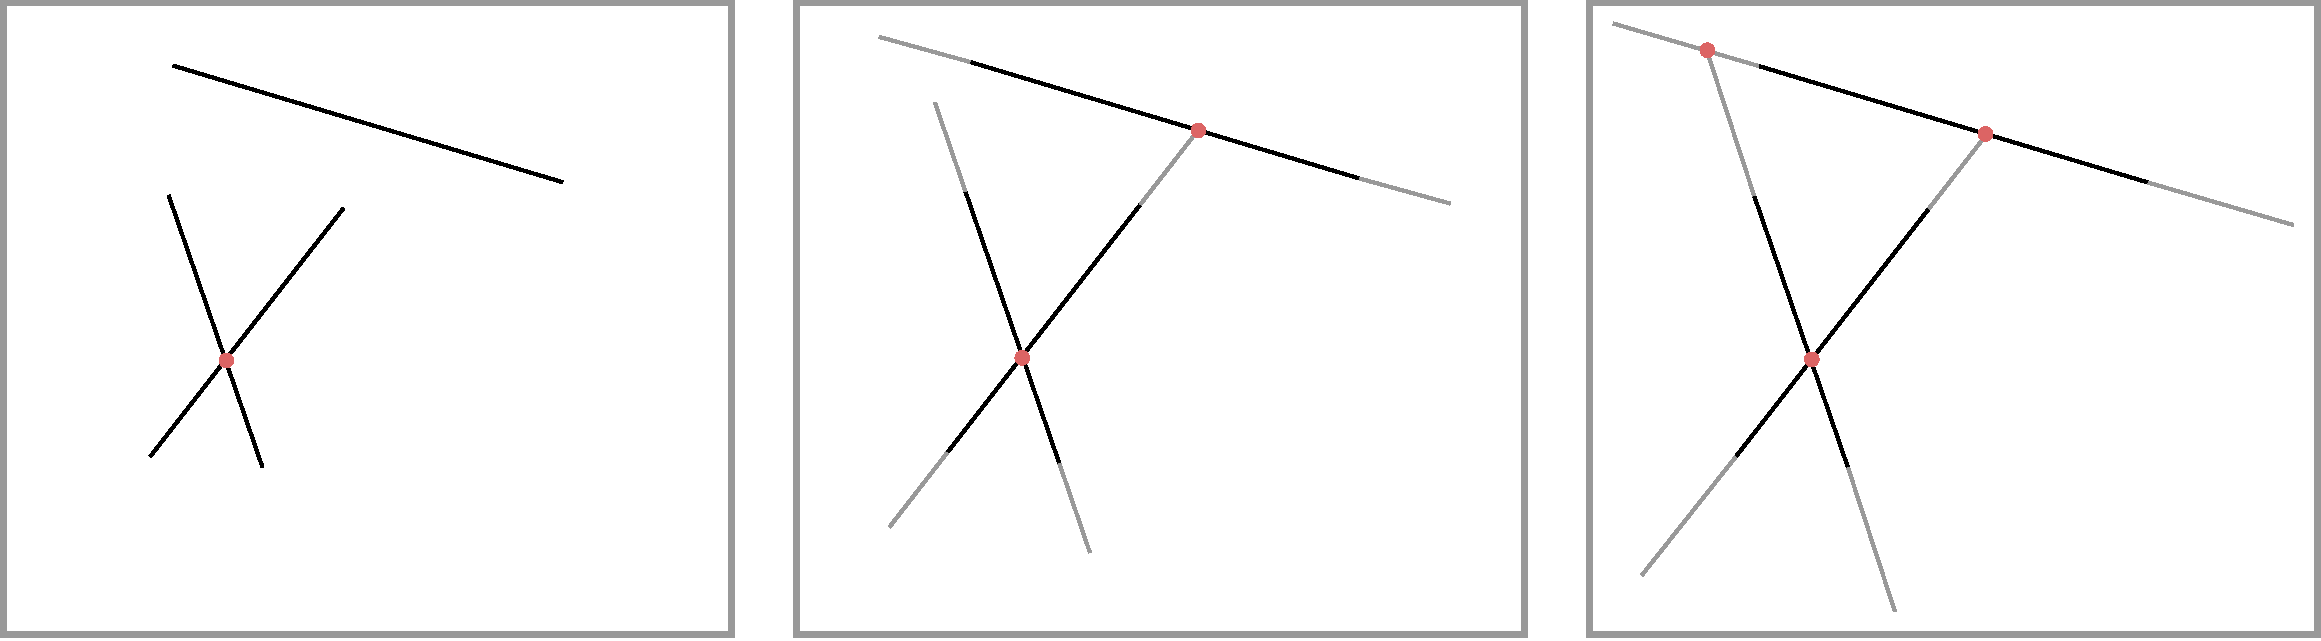
\includegraphics[width=\linewidth]{kinetic}

	Many \textbf{collinear segments} in this representation.
\end{frame}

\begin{frame}{Lifted model}
	\scriptsize
	\textbf{MRF formulation}
	\[
		E(\mathcal{L}) = \sum_{\mathcal{C}_i \in \mathcal{C}} E_{\mathcal{C}_i}(\mathcal{L}(\mathcal{C}_i)) + \mu \sum_{e = C_i \cap C_j} V_e(\mathcal{L}(\mathcal{C}_i), \mathcal{L}(\mathcal{C}_j))
	\]
	
	\begin{minipage}{0.6\linewidth}
		\textbf{Fidelity to ``inlier data''}
		\[
			E_{\mathcal{C}_i}(\Pi_k) = \frac{ \mathcal{A}_{\mathcal{C}_i}}{\operatorname{Card}(\mathbf{P}\cap \mathcal{C}_i)} \sum_{p \in \mathbf{P} \cap \mathcal{C}_i} \min(\epsilon, | p_z - \Pi_k(p_x, p_y) |)
		\]
		
		\textbf{Regularity to height jumps}
		\[ V_{e}(\Pi_k, \Pi_l) = p_e \operatorname{length}(e) \operatorname{z_e}(\Pi_k, \Pi_l) \]
	\end{minipage}%
	\begin{minipage}{0.4\linewidth}
		\centering
		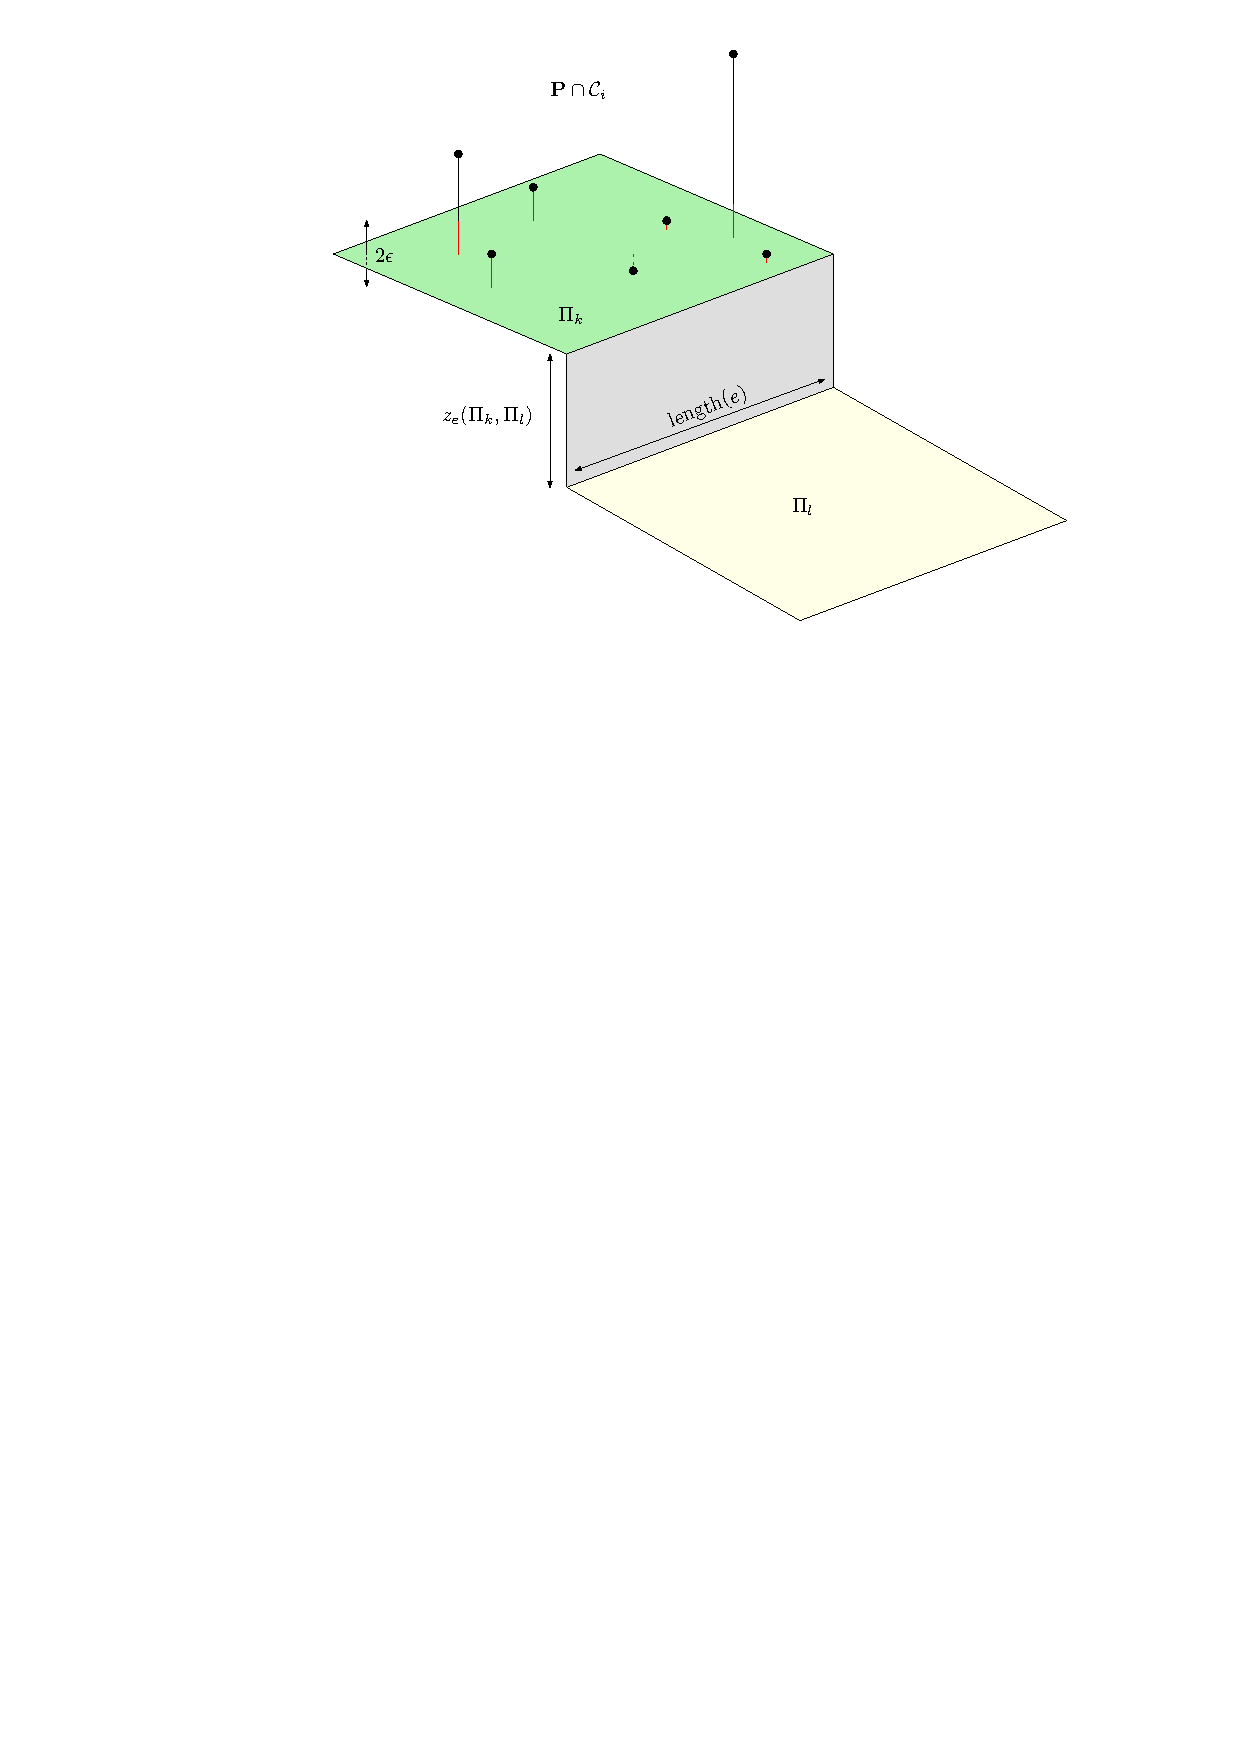
\includegraphics[width=\linewidth]{lift_terms}
	\end{minipage}
	\vspace{0.5cm}
	
	Local minima by \textbf{graph-cut optimization} \cite{boykov_FastApproximateEnergy_2001}.
\end{frame}

\begin{frame}{The need for simplification}
	\begin{figure}
		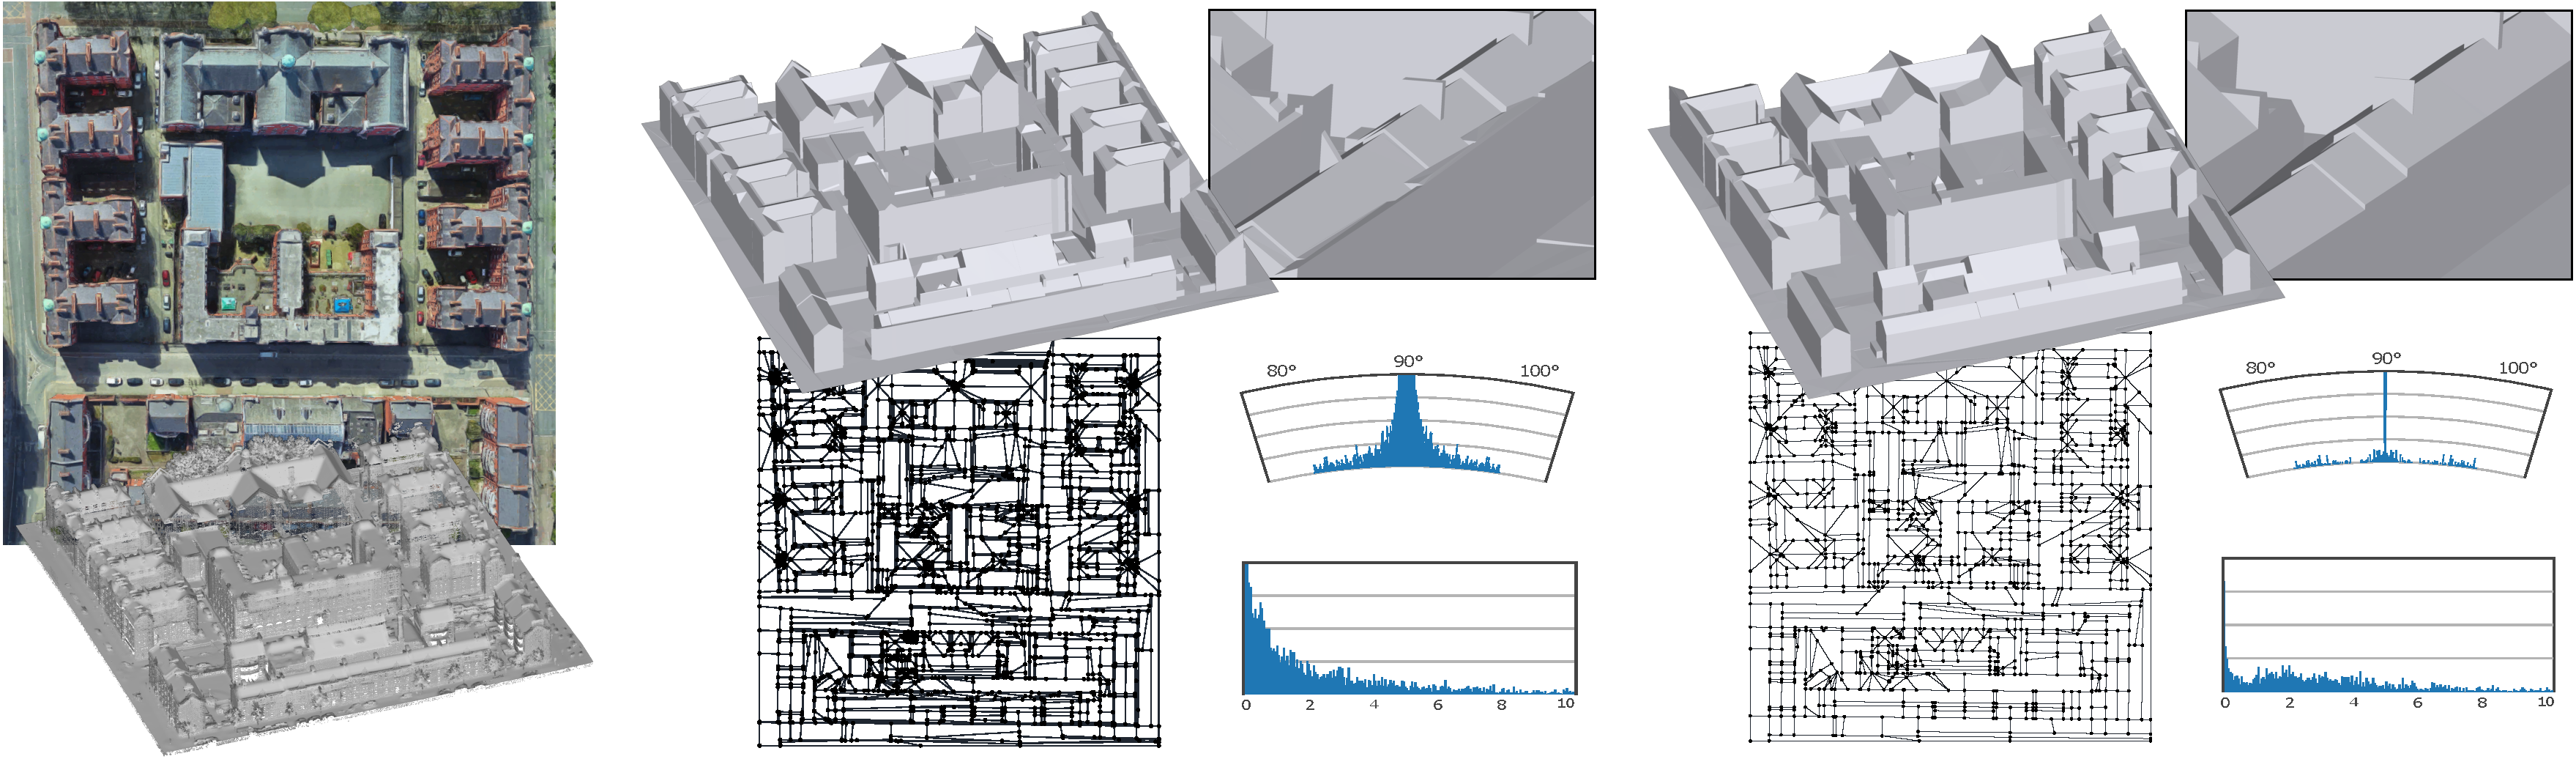
\includegraphics[width=\linewidth]{teaser_v2}
	\end{figure}
	
	\textbf{Complex} 2D partitions\\
	\textbf{Lack regularity} (small segments, angles close to orthogonality)\\
	Collinear segments \textbf{by design}\\
		
	\blfootnote{Dataset from 2015 LiDAR survey of Dublin \cite{laefer_2015AerialLaser_2017}.}
\end{frame}

\begin{frame}{Simplification of 2D partitions}
	\scriptsize
	\textbf{Related point set simplification problems}
	\begin{itemize}
		\item Geometric unit disk cover
		\item Minimum dominating set on unit disk graph
	\end{itemize}
	\textbf{NP-hard} \cite{marathe_SimpleHeuristicsUnit_1995}.
	
	\textbf{Simplification/regularity methods for urban scenes}
	\begin{itemize}
		\item Regularity in input data \cite{zhou_5DDualContouring_2010, monszpart_RAPterRebuildingManmade_2015}
		\item Discrete operations on the partitions \cite{li_ApproximatingShapesImages_2020}
		\item Output mesh simplification \cite{garland_SurfaceSimplificationUsing_1997, salinas_StructureAwareMeshDecimation_2015}
	\end{itemize}

	\textbf{Proposition:} Continuous simplification scheme on 2D partitions.
\end{frame}

\begin{frame}[t]{Point vs. line movement}
	\scriptsize
	
	\begin{minipage}{0.6\linewidth}
		\textbf{Point representation}
		\begin{itemize}
			\item Explicit coordinates for each point.
			\item Lines defined implicitly using two points.
		\end{itemize}	
		\begin{itemize}
			\item[\cmark] Multiple lines can share a same point.
			\item[\xmark] A line cannot carry more than two points.
		\end{itemize}
		
		Preserving collinearities \\
		\hspace{0.05cm} $\implies$ Optimization under constraints.
		
	\end{minipage}%
	\begin{minipage}{0.4\linewidth}
		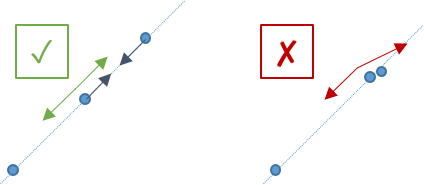
\includegraphics[width=\linewidth]{point_mouvement}
	\end{minipage}

	\vspace{0.5cm}
	\pause
	
	\textbf{Line representation}
	\begin{itemize}
		\item Explicit coordinates for each line.
		\item Points defined implicitly using two lines.
	\end{itemize}
	\begin{itemize}
		\item[\cmark] A line can carry more than two points.
		\item[\xmark] Multiple lines cannot share a same point.
	\end{itemize}
\end{frame}

\begin{frame}{Optimization on line coordinates}
	\small
	
	\begin{minipage}{0.5\linewidth}
		\textbf{Representation of lines}
		\[ a x + b y + c = 0 \]
	
		\textbf{Euclidean normalization}
		\[ a^2 + b^2 = 1 \]
	\end{minipage}%
	\begin{minipage}{0.5\linewidth}
		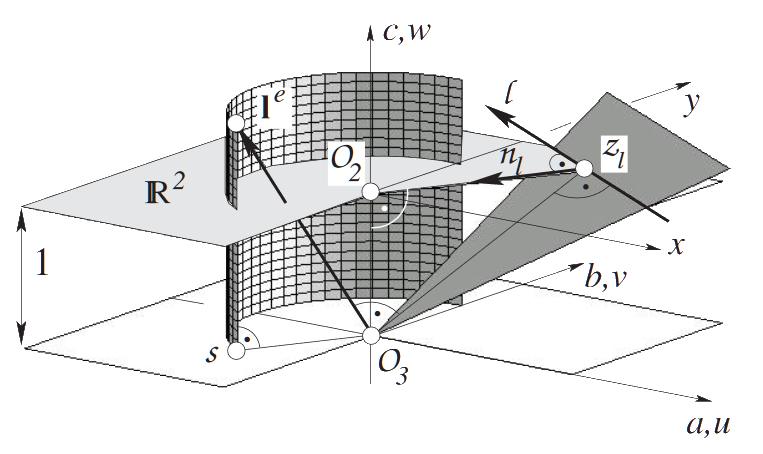
\includegraphics[width=\linewidth]{euclidean_normalization_line}
	\end{minipage}
	
	\vspace{1cm}
	
	\textbf{Trade-off between fidelity and regularity}
	\[ 
	E(\mathcal{L}) = E_{fidelity}(\mathcal{L}) + \lambda_1 \: E_{concurrent}(\mathcal{L}) + {\lambda_2} \: E_{orthogonality}(\mathcal{L})
	\]
	
	\blfootnote{Image from \cite{forstner_PhotogrammetricComputerVision_2016}.}
\end{frame}

\begin{frame}[t]{Fidelity term}
	\tiny
	\begin{flalign*}
		&E(\mathcal{L}) = \alert{E_{fidelity}(\mathcal{L})} + \lambda_1 \: E_{concurrent}(\mathcal{L}) + 	{\lambda_2} \: E_{orthogonality}(\mathcal{L})&
	\end{flalign*}
	
	\small
	\textbf{Fidelity term}

	No distance between lines invariant under Euclidean isometries.
	\begin{eqnarray*}
		d(P, L + \delta L)^2 & = & (\delta a \cdot x + \delta b \cdot y + \delta c)^2 \\
		& = &  {\delta L}^t
		\begin{pmatrix}
			x^2 & xy & x \\
			yx & y^2 & y \\
			x & y & 1
		\end{pmatrix} 
		\delta L
	\end{eqnarray*}
	\pause
	\[
		M_i \defunder{=} \frac{1}{2} 
		\begin{bmatrix}
			x_0^2 + x_1^2 + l_{\min}^2 & x_0 y_0 + x_1 y_1 & x_0 + x_1 \\
			x_0 y_0 + x_1 y_1 & y_0^2 + y_1^2  + l_{\min}^2 & y_0 + y_1 \\
			x_0 + x_1  & y_0 + y_1 & 2 
		\end{bmatrix}
	\]
	
	\pause
	\[
		E_{fidelity}(\mathcal{L}) \defunder{=} \frac{1}{2} \sum_{i = 1}^{n} L_i^t M_i L_i
	\]
\end{frame}

\begin{frame}[t]{Regularity terms}
	\tiny
	\begin{flalign*}
		&E(\mathcal{L}) = E_{fidelity}(\mathcal{L}) + \lambda_1 \: \alert{E_{concurrent}(\mathcal{L})} + {\lambda_2} \: \alert{E_{orthogonality}(\mathcal{L})}&
	\end{flalign*}

	\small
	\begin{minipage}{0.7\linewidth}
	\textbf{Line concurrency}
	\begin{eqnarray*}
		D_{ijk} &\defunder{=}& |\det(L_i, L_j, L_k)| \\
		& = & ||P_{ij} - P_{ik}|| \sin \alpha_{ij} \: \sin \alpha_{ik}
	\end{eqnarray*}
	\end{minipage}%
	\begin{minipage}{0.3\linewidth}
		\centering
		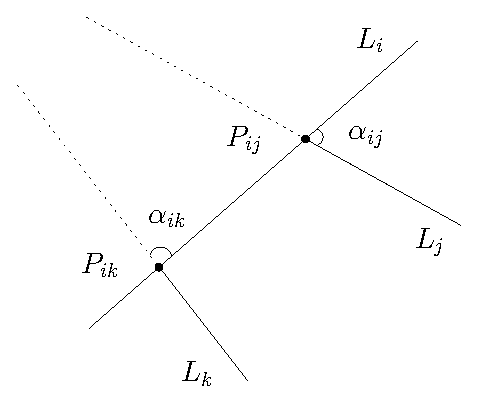
\includegraphics[width=\linewidth]{concurrent_config}
	\end{minipage}%
	\[
		E_{concurrent}(\mathcal{L}) = \sum_{(i, j, k) \in \mathcal{T}} \min \left(\epsilon, |\det(L_i, L_j, L_k)| \right)
	\]
	
	\vspace{0.5cm}
	\textbf{Orthogonality}
	\[
		E_{orthogonality}(\mathcal{L}) = \sum_{(i, j) \in \mathcal{P}} \min (\sin \alpha_{\max}, |\operatorname{dot2d}(L_i, L_j) |)
	\]
\end{frame}

\begin{frame}[c]{Riemannian gradient descent (I)}
	\scriptsize
	
	\begin{minipage}[t]{0.5\linewidth}
		\textbf{Euclidean case:} $\nabla f = D^{t}$
	\end{minipage}%
	\pause%
	\begin{minipage}[t]{0.5\linewidth}
		\centering
 		\textbf{Riemannian manifold:} $\nabla f = G^{-1} D^t$
	\end{minipage}%
	
	\begin{center}
	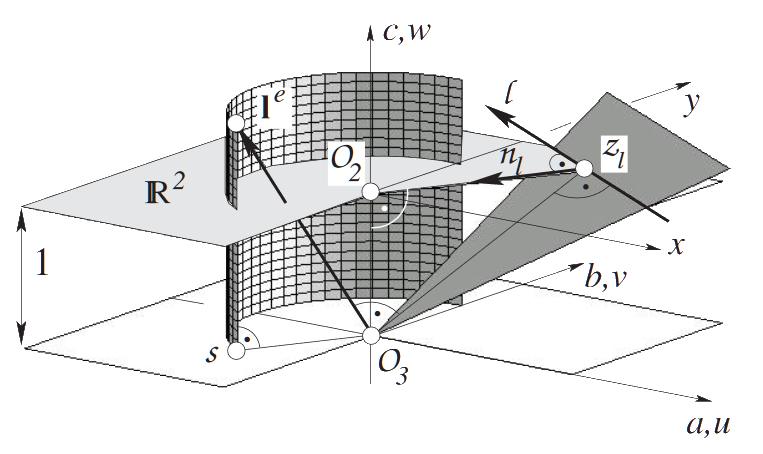
\includegraphics[width=0.5\linewidth]{euclidean_normalization_line}
	\end{center}

	\textbf{Tangent space} of $\mathcal{M}$ at $L_i$:
	\begin{tabular}{cc}
		$ \mathcal{T}_{L_i} \mathcal{M} = \{ v \in \mathbb{R}^3, v \cdot (a,b, 0) = 0 \} = U_i \mathbb{R}^2 $
		& with $U_i = \begin{pmatrix} b & 0 \\ a & 0 \\ 0 & 1 \end{pmatrix}$
	\end{tabular}

	$M_i$, restricted to this $2$-dimensional vector space $\mathcal{T}_{L_i} \mathcal{M}$, is \textbf{non-degenerate}.
%	: it defines a Riemannian metric for the line $L_i$ on $\mathcal{M}$.
\end{frame}

\begin{frame}[c]{Riemannian gradient descent (II)}
	\scriptsize

	\textbf{Derivative} of the objective function
	\[ D_i = \left( \frac{dE }{da},  \frac{dE }{db}, \frac{dE }{dc} \right) \]	
	
	\textbf{Derivative and Riemannian metric} in the tangent space $\mathcal{T}_{L_i} \mathcal{M}$:
	\begin{eqnarray*}
		D_i' &=& D_i U_i \\
		M_i' &=& U_i^t  M_i U_i
	\end{eqnarray*}
	
	\textbf{Gradient} in homogeneous coordinates:
	\[
	\nabla_i E = U_i (M_i')^{-1} {D_i'}^t
	\]
	
	\textbf{Gradient descent} step:
	\[
	\forall i,  \quad L_i^{(k+1)} = normalize\left(  L_i^{(k)} - \alpha \nabla_i E   \right) 
	\]
\end{frame}

\begin{frame}{Combinatorial reductions}
	\scriptsize

	\textbf{Discrete simplification operations}: merging lines.
		
	Two possibilities for $|\det(L_i, L_j, L_k) | = 0$
	\begin{enumerate}
		\item[a.] Two equal lines;
		\item[b.] Lines meets at a same point.
	\end{enumerate}
	
	Special care when using a threshold: $|\det(L_i, L_j, L_k) | < \eta$.
	\pause
	
	\begin{minipage}{0.7\linewidth}
	Merging lines $L_i, L_j$ into $L_f$:
	\[ M_f = M_i + M_j \]
	
	Similar to QEM \cite{garland_SurfaceSimplificationUsing_1997}.
	\end{minipage}%
	\begin{minipage}{0.3\linewidth}
		\centering
		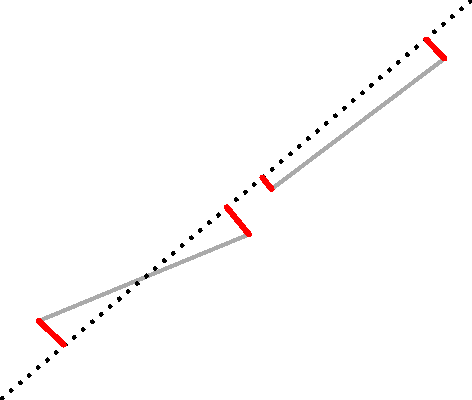
\includegraphics[height=0.6\linewidth]{metric_merge}
	\end{minipage}
\end{frame}

\begin{frame}[c]{Optimization}
	\begin{center}
		\begin{overpic}[width=\textwidth]{arrangement_levels}		
			\put(10,33){\makebox[0pt]{\fontsize{6}{6}\textsc{Iteration 0}}}
			\put(10,31){\makebox[0pt]{\fontsize{6}{6}\selectfont{Complexity: 1,121}}}
			\put(10,29){\makebox[0pt]{\fontsize{6}{6}\selectfont{Orthogonality: 0}}}
			
			\put(30,33){\makebox[0pt]{\fontsize{6}{6}\textsc{Iteration 1000}}}
			\put(30,31){\makebox[0pt]{\fontsize{6}{6}\selectfont{Complexity: 812}}}
			\put(30,29){\makebox[0pt]{\fontsize{6}{6}\selectfont{Orthogonality: 529}}}
			
			\put(50,33){\makebox[0pt]{\fontsize{6}{6}\textsc{Iteration 3000}}}
			\put(50,31){\makebox[0pt]{\fontsize{6}{6}\selectfont{Complexity: 518}}}
			\put(50,29){\makebox[0pt]{\fontsize{6}{6}\selectfont{Orthogonality: 391}}}
			
			\put(70,33){\makebox[0pt]{\fontsize{6}{6}\textsc{Iteration 7000}}}
			\put(70,31){\makebox[0pt]{\fontsize{6}{6}\selectfont{Complexity: 137}}}
			\put(70,29){\makebox[0pt]{\fontsize{6}{6}\selectfont{Orthogonality: 161}}}
			
			\put(90,33){\makebox[0pt]{\fontsize{6}{6}\textsc{Iteration 9000}}}
			\put(90,31){\makebox[0pt]{\fontsize{6}{6}\selectfont{Complexity: 44}}}
			\put(90,29){\makebox[0pt]{\fontsize{6}{6}\selectfont{Orthogonality: 57}}}
		\end{overpic}
	\end{center}
\end{frame}

\begin{frame}{Comparison}
	\centering
	\tiny
	\begin{overpic}[width=0.9\linewidth]{comparisons_v2}
		%Laser
		\put(0,30){\fontsize{7}{7}\selectfont{LiDAR}}
		
		\put(30,56.5){\fontsize{7}{7}\selectfont{QEM}}
		\put(45,46.5){\fontsize{5}{5}\selectfont{error: 0.079}}
		\put(45,45.5){\fontsize{5}{5}\selectfont{complexity: 15}}
		
		\put(30,42.5){\fontsize{7}{7}\selectfont{SAMD}}
		\put(45,33.5){\fontsize{5}{5}\selectfont{error: 0.085}}
		\put(45,32.5){\fontsize{5}{5}\selectfont{complexity: 16}}
		
		\put(54,56.5){\fontsize{7}{7}\selectfont{RPP}}
		\put(69,46.5){\fontsize{5}{5}\selectfont{error: 0.032}}
		\put(69,45.5){\fontsize{5}{5}\selectfont{complexity: 814}}
		
		\put(54,42.5){\fontsize{7}{7}\selectfont{VSA}}
		\put(69,33.5){\fontsize{5}{5}\selectfont{error: 0.072}}
		\put(69,32.5){\fontsize{5}{5}\selectfont{complexity: 501}}
		
		\put(76,56.5){\fontsize{7}{7}\selectfont{Ours (w/o simpl.)}}
		\put(93,46.5){\fontsize{5}{5}\selectfont{error: 0.074}}
		\put(93,45.5){\fontsize{5}{5}\selectfont{complexity: 33}}
		
		\put(76,42.5){\fontsize{7}{7}\selectfont{Ours}}
		\put(93,33.5){\fontsize{5}{5}\selectfont{error: 0.054}}
		\put(93,32.5){\fontsize{5}{5}\selectfont{complexity: 15}}
		
		%MVS
		\put(0,25){\fontsize{7}{7}\selectfont{Photogrammetry}}
		
		\put(30,25){\fontsize{7}{7}\selectfont{QEM}}
		\put(45,16){\fontsize{5}{5}\selectfont{error: 0.097}}
		\put(45,15){\fontsize{5}{5}\selectfont{complexity: 24}}
		
		\put(30,12.5){\fontsize{7}{7}\selectfont{SAMD}}
		\put(45,3){\fontsize{5}{5}\selectfont{error: 0.07}}
		\put(45,2){\fontsize{5}{5}\selectfont{complexity: 25}}
		
		\put(54,25){\fontsize{7}{7}\selectfont{RPP}}
		\put(69,16){\fontsize{5}{5}\selectfont{error: 0.044}}
		\put(69,15){\fontsize{5}{5}\selectfont{complexity: 28}}
		
		\put(54,12.5){\fontsize{7}{7}\selectfont{VSA}}
		\put(69,3){\fontsize{5}{5}\selectfont{error: 0.03}}
		\put(69,2){\fontsize{5}{5}\selectfont{complexity: 717}}
		
		\put(76,25){\fontsize{7}{7}\selectfont{Ours (w/o simpl.)}}
		\put(93,16){\fontsize{5}{5}\selectfont{error: 0.07}}
		\put(93,15){\fontsize{5}{5}\selectfont{complexity: 186}}
		
		\put(76,12.5){\fontsize{7}{7}\selectfont{Ours}}
		\put(93,3){\fontsize{5}{5}\selectfont{error: 0.055}}
		\put(93,2){\fontsize{5}{5}\selectfont{complexity: 24}}
	\end{overpic}
\end{frame}

\begin{frame}[c]{Results}
	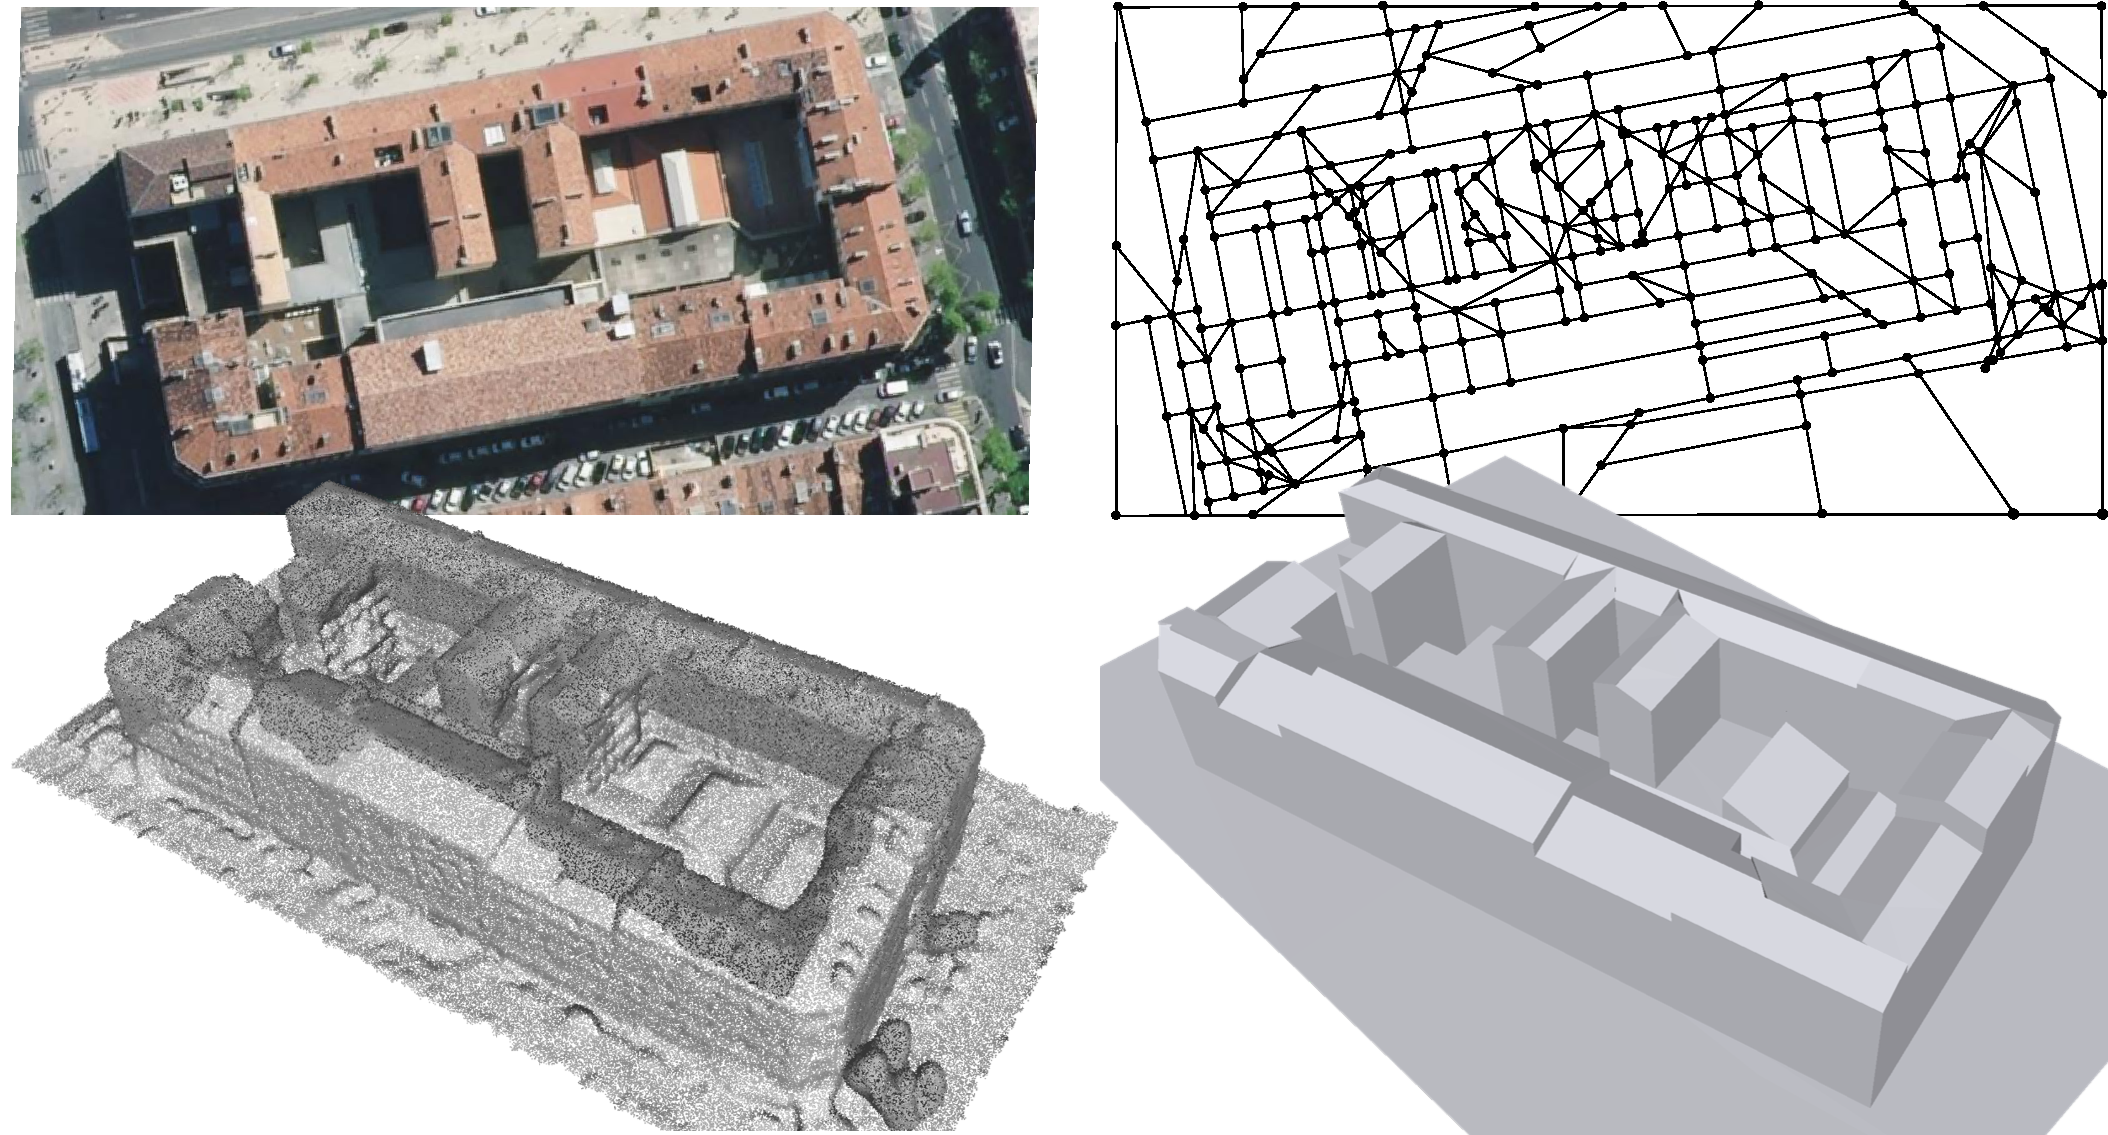
\includegraphics[width=0.5\linewidth]{bb_v2}%
	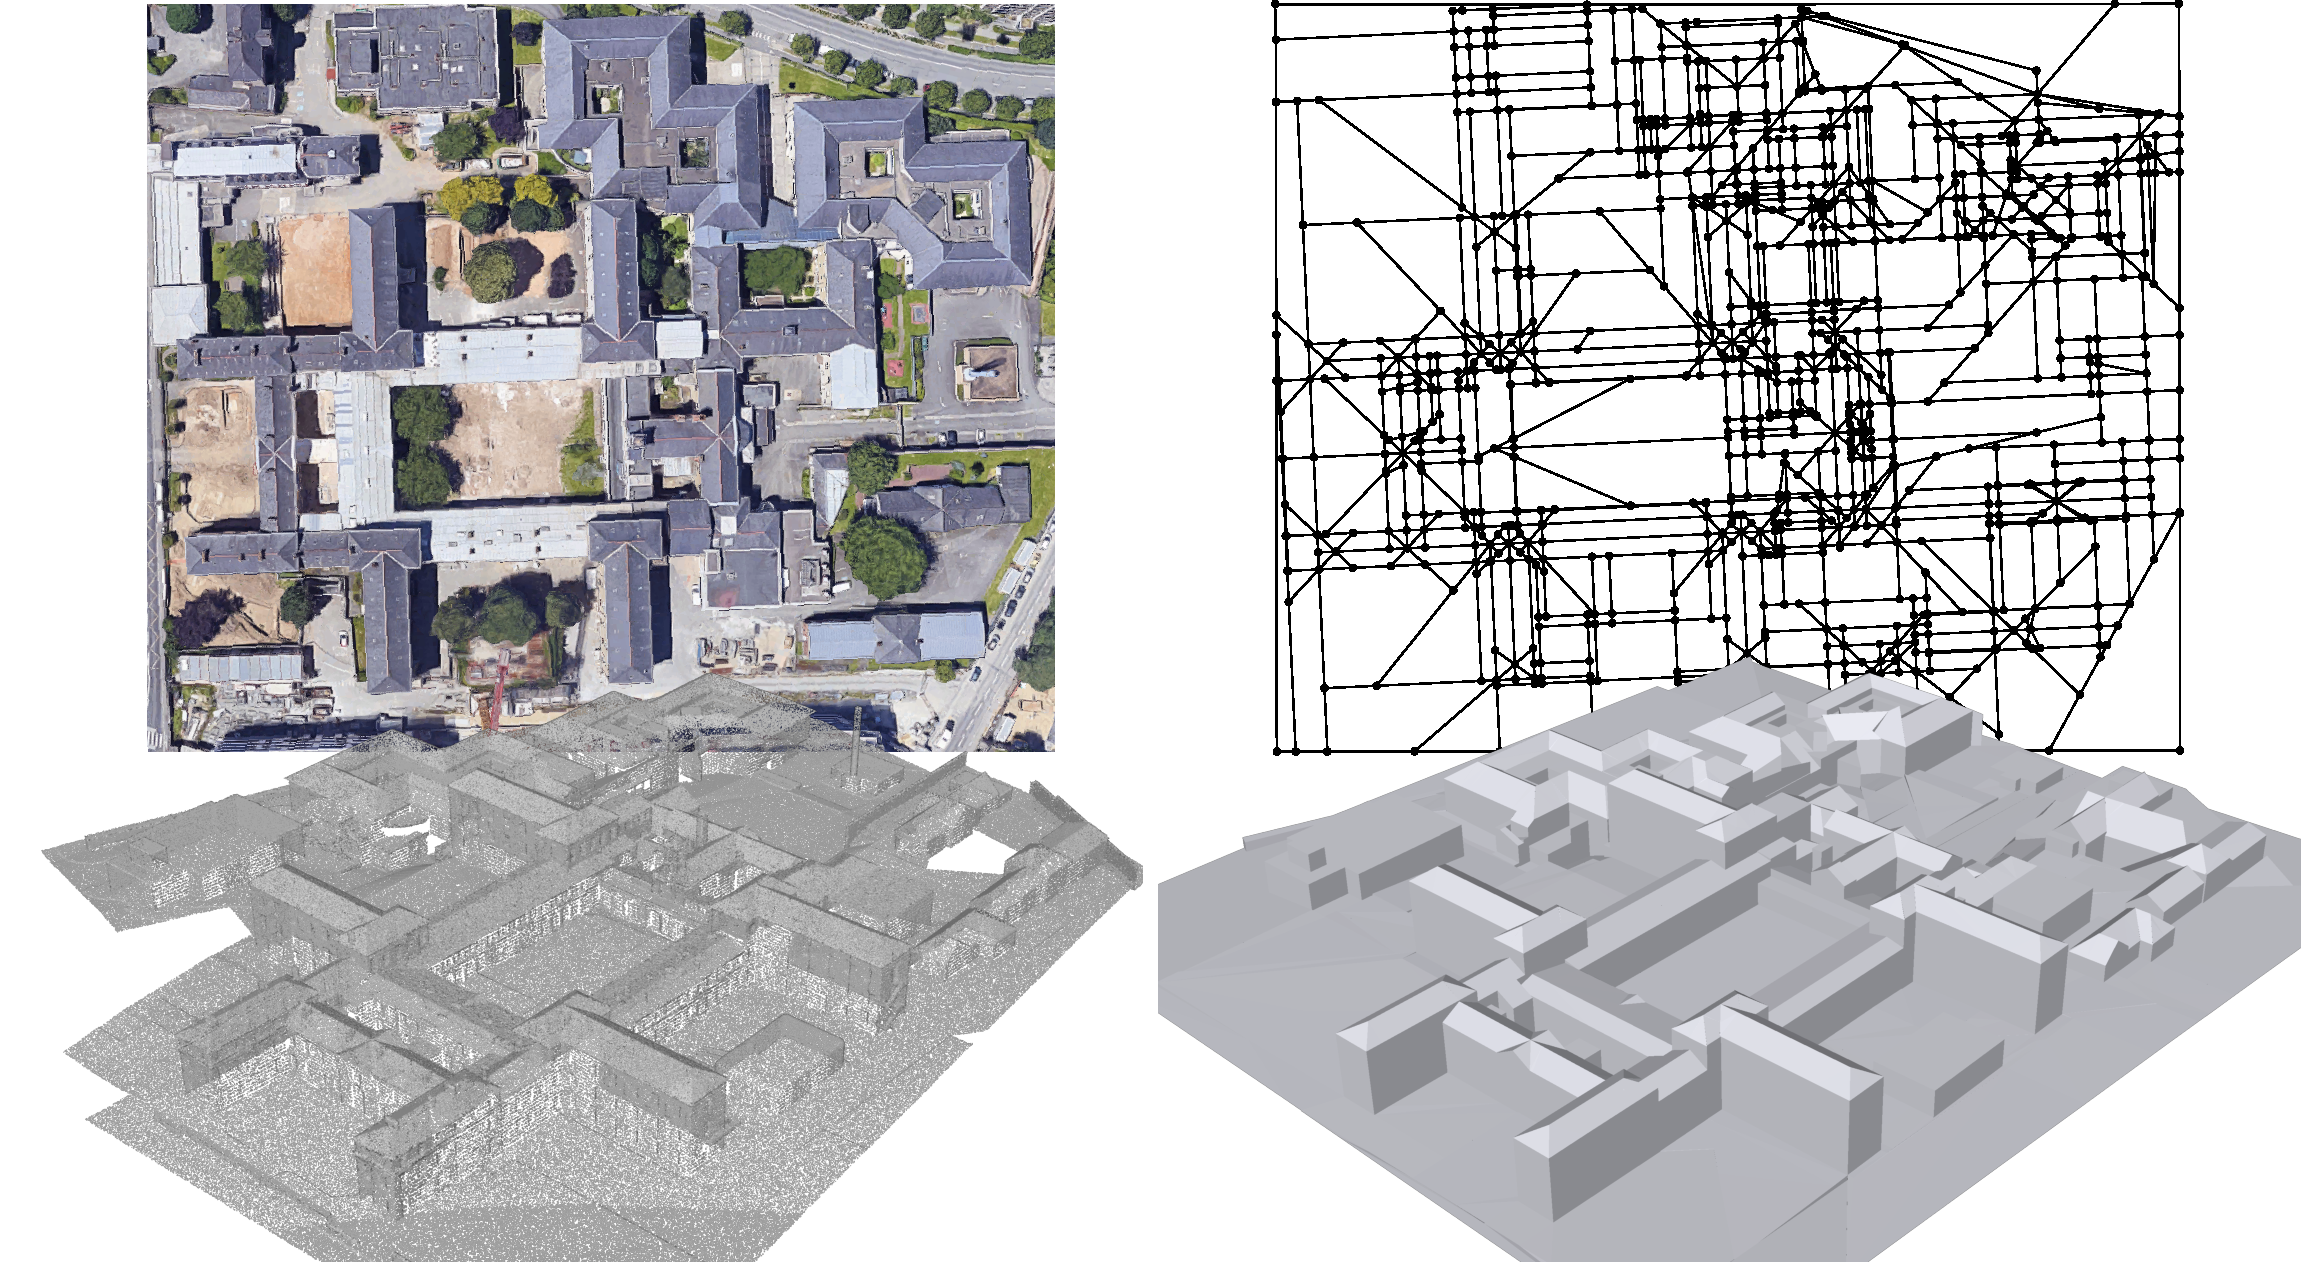
\includegraphics[width=0.5\linewidth]{hoteldieu_v3}
\end{frame}

\begin{frame}{Limitations}
	\small
	\textbf{Representability} of the LOD2 model
	\begin{center}
		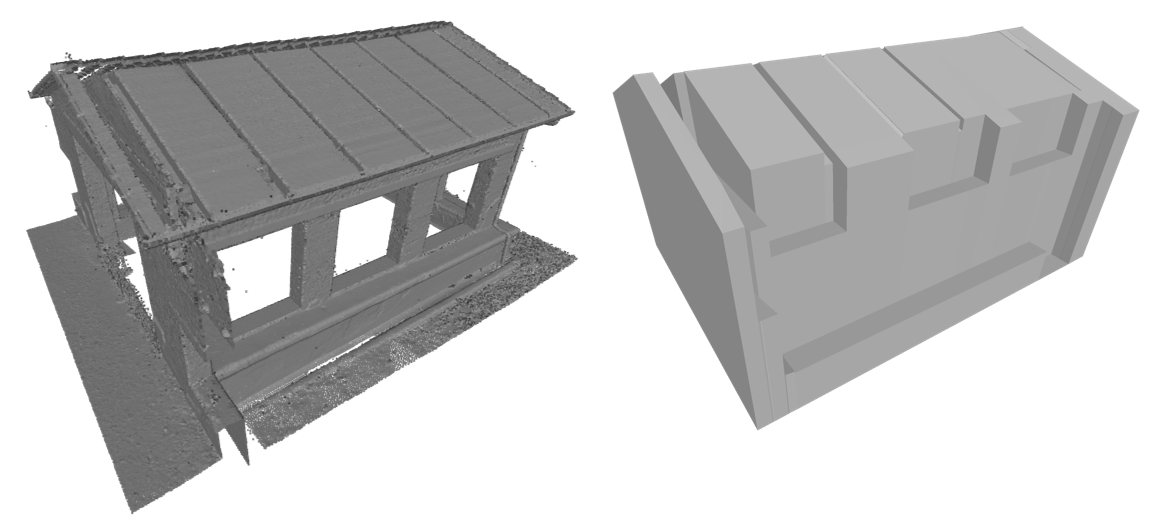
\includegraphics[width=0.6\linewidth]{failure_case}
	\end{center}

	\textbf{Dissociation} between 2D and 3D regularity
	\begin{center}
		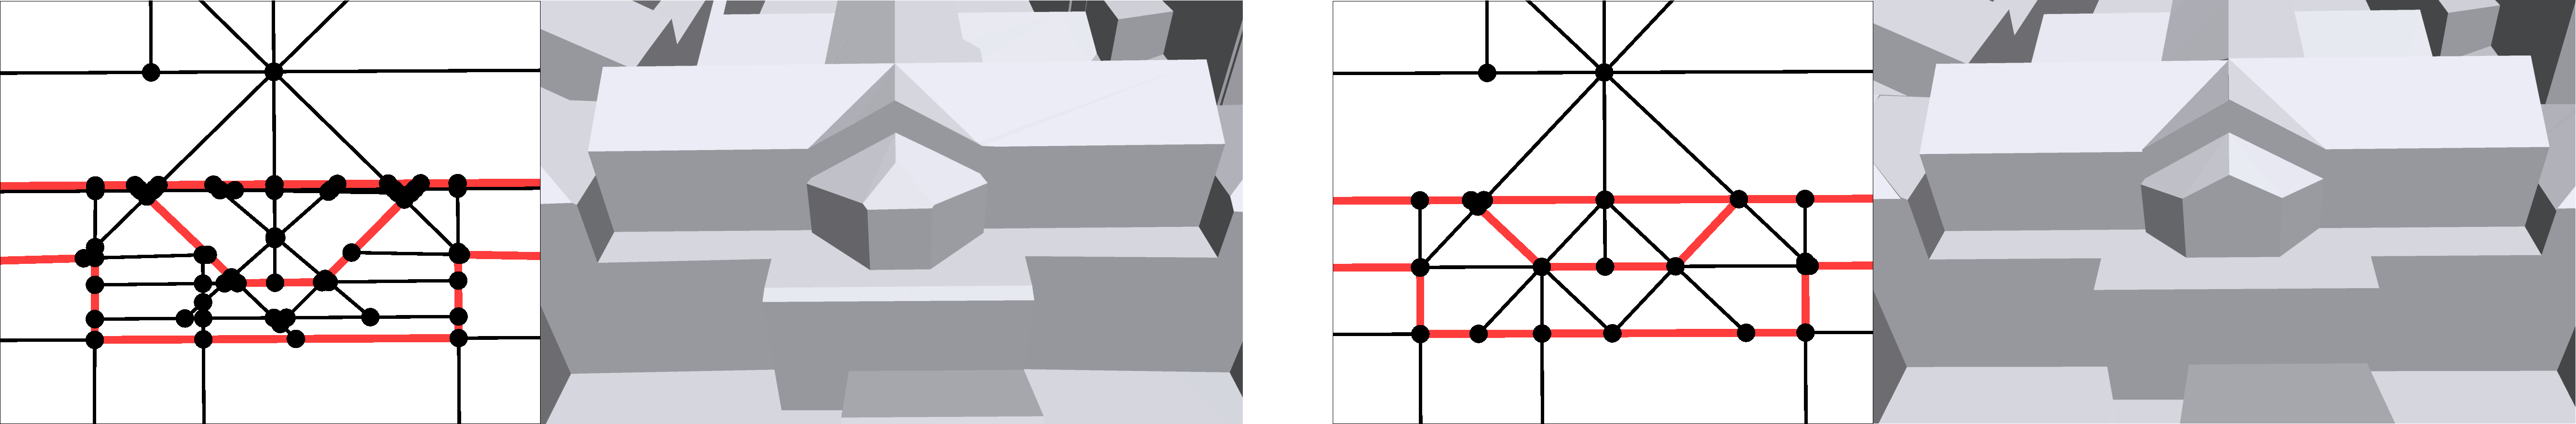
\includegraphics[width=0.8\linewidth]{closeup_v2}
	\end{center}
\end{frame}

	\section{Dense representations from lexicographic optimal chains}

\graphicspath{{images/lexicographic}}

% Intuition
\begin{frame}[c]{Intuition}
	\centering
	\newcommand{\legendsize}{6pt}
	\tikzset{legend/.style = {rectangle, text width=0.2\linewidth}}
	\begin{tikzpicture}
		\onslide<1>{
			\node (pointcloud)
			{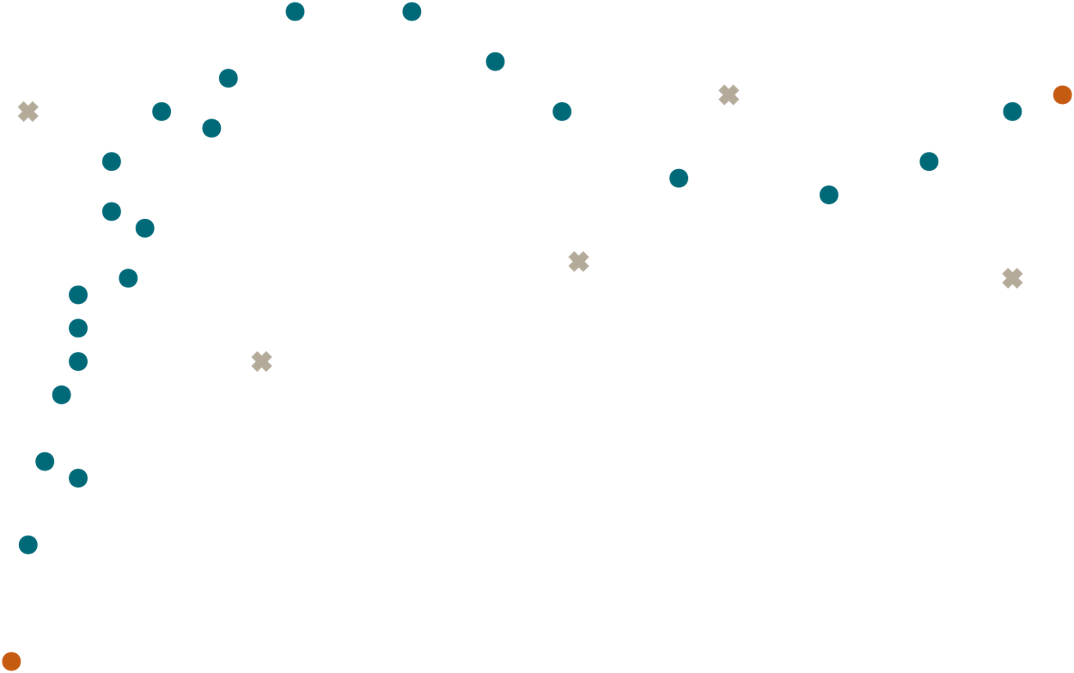
\includegraphics[width=0.8\linewidth]{intuition/state_0}};
		}
		\onslide<2>{
			\node (pointcloud)
			{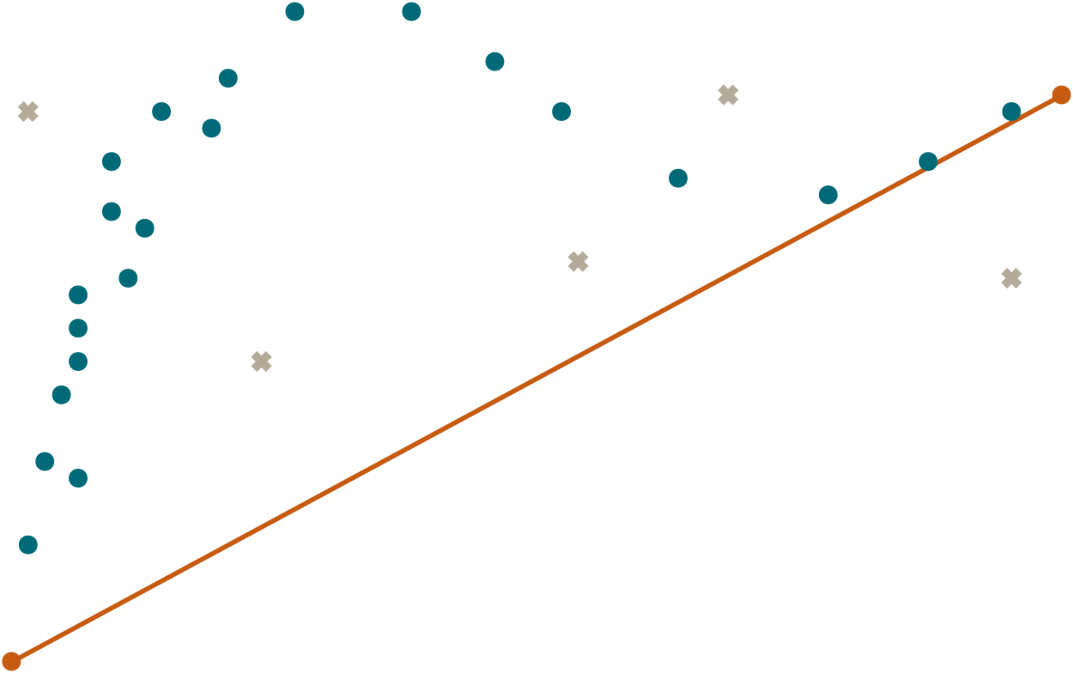
\includegraphics[width=0.8\linewidth]{intuition/state_1}};
		}
		\onslide<3>{
			\node (pointcloud)
			{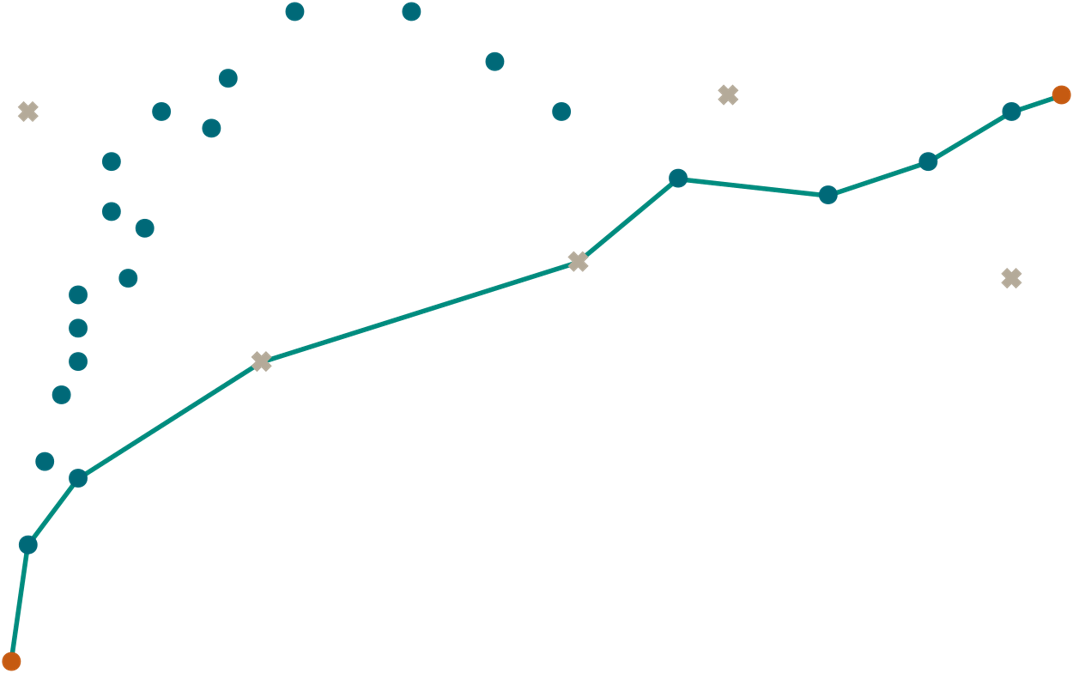
\includegraphics[width=0.8\linewidth]{intuition/state_2}};
		}
		\onslide<4>{
			\node (pointcloud)
			{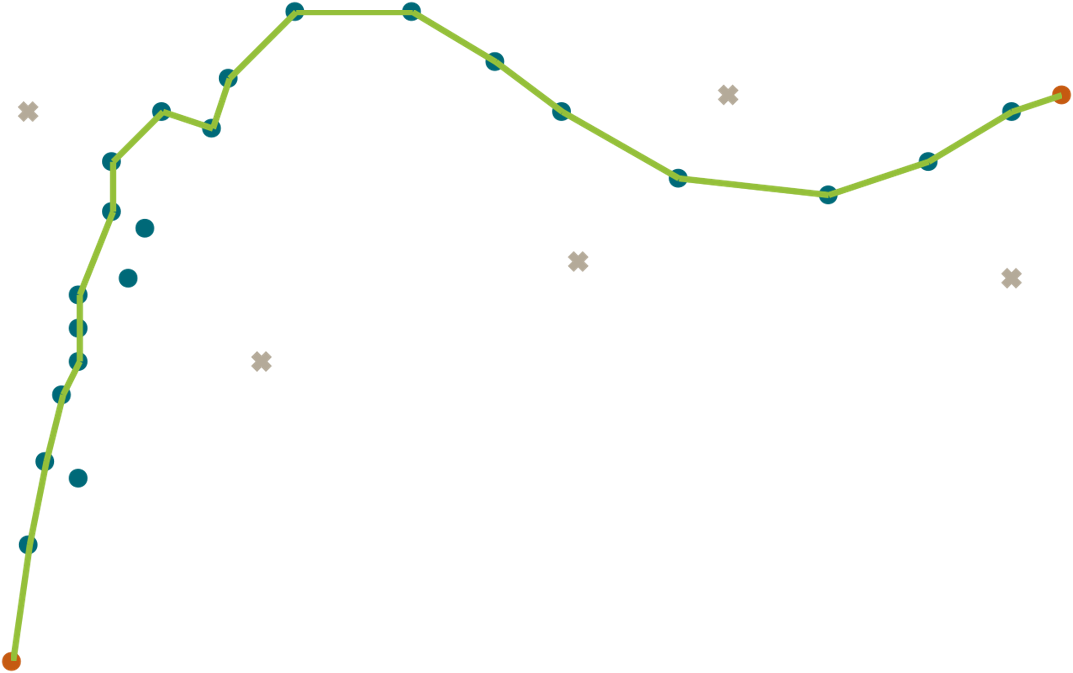
\includegraphics[width=0.8\linewidth]{intuition/state_3}};
		}
		\node[legend, anchor=south east] at (pointcloud.south east){
			\fontsize{\legendsize}{9pt}\selectfont
			\begin{itemize}[itemsep=0pt,partopsep=0pt,topsep=0pt]
				\item[{
\includegraphics[width=\legendsize]{intuition/inlier}}]{Inlier}
				\item[{
\includegraphics[width=\legendsize]{intuition/endpoint}}]{Endpoint}
				\item[{
\includegraphics[width=\legendsize]{intuition/outlier}}]{Outlier}
			\end{itemize}
		};
	\end{tikzpicture}
	
	\vspace*{0.5cm}
	
	\begin{tabular}{ccc}
		\visible<2->{\small\color{pathorange}
		$\min_P \sum_{e \in P} \length(e)^{~}$	
		} & 
		\visible<3->{\small\color{pathblue}
		$\min_P \sum_{e \in P} \length(e)^2$} &
		\visible<4->{\small\color{pathgreen}
		$\min_P \sum_{e \in P} \length(e)^p$
		}
	\end{tabular}
\end{frame}

% Lexicographic order
\begin{frame}[c]{Limit behaviour when $p \rightarrow \infty$}
	Total order on edges based on their length: $e_1 > e_2 > \dots > e_n$
	\pause
	
	There is a $p$ large enough such that, for all $i=1,\dots,n$:
	\[
		\length(e_i)^p > \sum_{j > i} \length(e_j)^p
	\]
	
	\pause
	$\mathcal{P}_1 = \{ e_1, e_2, \cdots, e_m \}$ with $e_1 > e_2 > \cdots > e_m$.
	$\mathcal{P}_2 = \{ e'_1, e'_2, \cdots, e'_p \}$ with $e'_1 > e'_2 > \cdots > e'_p$.
\end{frame}

% Total order on k-simplices
\begin{frame}{A total order based on the Delaunay triangulation}
	\scriptsize
	\begin{center}
		\begin{minipage}{0.5\linewidth}
			\centering
			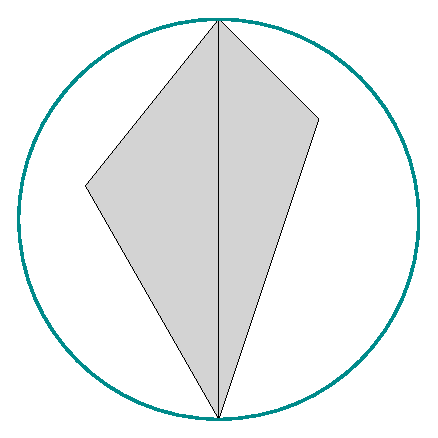
\includegraphics[height=0.3\textheight]{order_rseb}\\
			\color{pathblue}$\rseb(\sigma_1) = \rseb(\sigma_2)$	
		\end{minipage}%
		\begin{minipage}{0.5\linewidth}
			\centering
			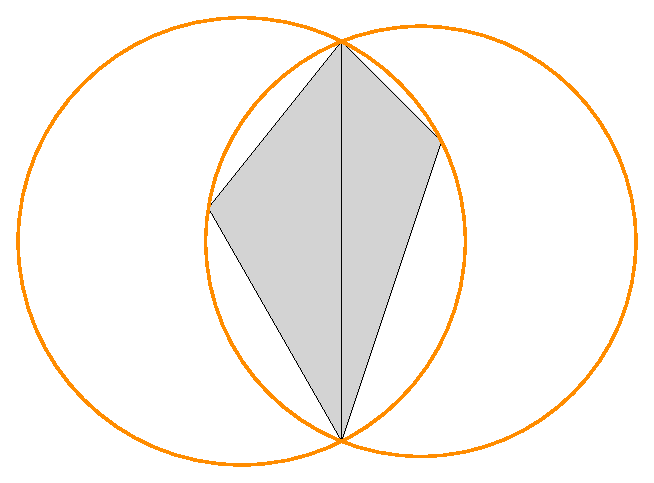
\includegraphics[height=0.3\textheight]{order_rcirc}\\
			\color{pathorange} $\circrad(\sigma_1) \neq \circrad(\sigma_2)$
		\end{minipage}%
	\end{center}
	
	\vspace{0.5cm}
	
	\begin{block}{Total order on 2-simplices}
		For $\sigma_1, \sigma_2 \in K^{(2)}$,
		\[
		\sigma_1 \leq \sigma_2 \defunder{\iff}
		\begin{cases}
			\rseb(\sigma_1) < \rseb(\sigma_2) &\\
			\:  \operatorname{or} &\\
			\rseb(\sigma_1) = \rseb(\sigma_2) & \operatorname{and} \circrad(\sigma_1) \geq \circrad(\sigma_2)
		\end{cases}
		\]
	\end{block}
\end{frame}

% Crash course
\begin{frame}[c]{Simplicial homology}
	\begin{tabular}{cc}
		Simplices & \raisebox{-.5\height}{
\includegraphics[width=0.5\textwidth]{course/simplices}} \\
		Simplicial complex & \raisebox{-.5\height}{
\includegraphics[width=0.4\textwidth]{course/complex}}
	\end{tabular}
		
	\vspace{1cm}
	
	A \textbf{\textit{k}-chain} $A$ with coefficients in $\F$ is a formal sum of $k$-simplices:
	\begin{equation*}
		A = \sum_{i} x_i \sigma_i, \text{ with } x_i \in \F \; \text{and} \;\sigma_i \in K^{(k)}
	\end{equation*}
\end{frame}

\begin{frame}{Boundary operator}
	The \textbf{boundary operator} $\partial_k : \Cchains_{k}(K) \to \Cchains_{k-1}(K)$ is the linear map defined for any $k$-simplex $\sigma = [a_0, \dots, a_k]$ as:
	\[
	\partial_k \sigma  \defunder{=}\sum_{i=0}^{k} (-1)^{i} [a_0,\dots, \widehat{a_i},\dots, a_k]
	\]
	
	\begin{center}
		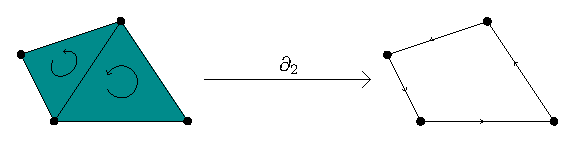
\includegraphics[width=0.8\textwidth]{course/boundary}
	\end{center}
\end{frame}

\begin{frame}{Cycles \& Boundaries}
	The kernels and images of the boundary operator form respectively the vector space of \textbf{cycles} and \textbf{boundaries}:
	\begin{align*}
		\Zchains_{k}(K) &\defunder{=} \Ker \partial_k = \Big\{ \Gamma \in \Cchains_{k}(K), \partial_k \Gamma = 0 \Big\} 
		%\label{definition:absolute-cycles}
		\\
		\Bchains_k(K) &\defunder{=} \Ima \partial_{k+1} = \Big\{ \Gamma \in \Cchains_{k}(K), \exists A \in \Cchains_{k+1}(K) \mid \Gamma = \partial_{k+1} A \Big\} 
		%\label{definition:absolute-boundaries}
	\end{align*}

	\[
		\partial_{k} \partial_{k+1} = 0 \iff \Bchains_k(K) \subset \Zchains_k(K)$
	\]	
	
	\begin{center}
		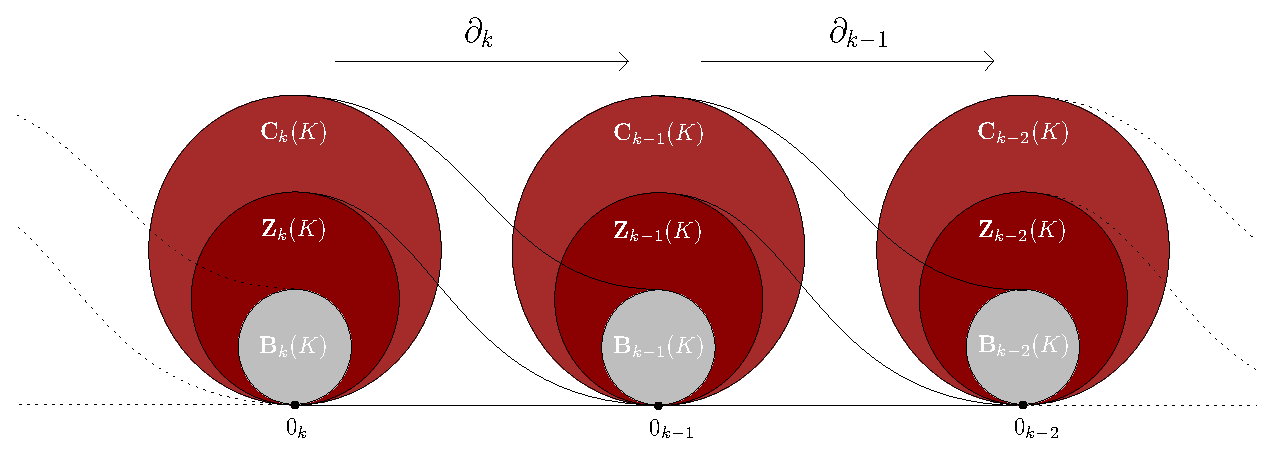
\includegraphics[width=0.5\linewidth]{course/sequence}
	\end{center}
\end{frame}
%
%\begin{frame}{Fundamental property}
%	\begin{tabular}{lcl}
%	$\partial_{k} \partial_{k+1} = 0$ && ``Boundaries have no boundaries'' \\
%	\pause
%	& $\iff$ & \\
%	$\Bchains_k(K) \subset \Zchains_k(K)$ && ``All boundaries are cycles''
%	\end{tabular}
%
%	\pause
%	\begin{center}
%		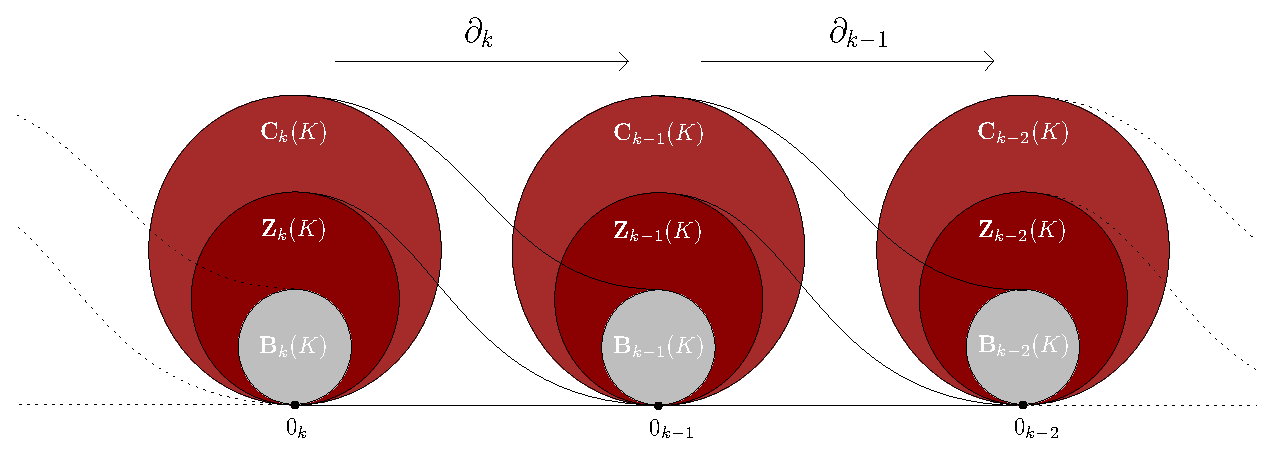
\includegraphics[width=0.9\textwidth]{course/sequence}
%	\end{center}
%\end{frame}

\begin{frame}{Simplicial homology}
\textbf{Homology groups} are defined as quotient spaces of cycles over boundaries:
\[
\Homol_k(K) \defunder{=} \frac{\Zchains_k(K)}{\Bchains_k(K)}
\]

$A, A' \in \Zchains_k(K)$ are \textbf{homologous cycles} \\
\pause
\vspace*{5pt}
\hspace*{5pt} $\defunder{\iff}$ they belong to the same homology class in $\Homol_k(K)$ \\
\pause
\vspace*{5pt}
\hspace*{5pt} $\iff A -  A' = \partial_{k+1}B$ for some ($k+1$)-chain $B$.

\begin{center}
\begin{tikzpicture}
	\node[help lines](torus) {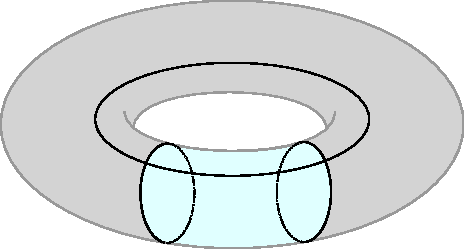
\includegraphics[width=0.5\linewidth]{course/homologous}};
	\node[below left=-1cm and -1.75cm of torus]{$A$};
	\node[below right=-1cm and -1.75cm of torus]{$A'$};
	\node[below=-0.8cm of torus]{$B$};
	\node[above=-0.8cm of torus]{$C$};
\end{tikzpicture}
\end{center}
\end{frame}

% Lexicographic order
\begin{frame}{Lexicographic preorder on chains}
	Total order on $k$-simplices, denoted $<$.\\
	
	\textbf{Lexicographic total preorder} Given $\Gamma_1, \Gamma_2 \in \Cchains_k(K; \F)$,
		\[
		\Gamma_1 \LexicographicOrderChain \Gamma_2 \defunder{\iff}
		\begin{cases} 
			|\Gamma_1| = |\Gamma_2| \\
			\operatorname{or} \\
			\max \big\{ \sigma \in |\Gamma_1| \triangle |\Gamma_2|  \big\}  \in |\Gamma_2|
		\end{cases}
		\]
		where $\triangle$ denotes the set symmetric difference.
		
	\[
		\big( \Gamma_1 \LexicographicOrderChain \Gamma_2 \quad \textrm{and} \quad  	\Gamma_2 
		\LexicographicOrderChain  \Gamma_1 \big) \iff |\Gamma_1| = |\Gamma_2| 
	\]
	
	\begin{alertblock}{$\F = \Z_2$}
		$\LexicographicOrderChain$ is a total order.
	\end{alertblock}
\end{frame}

% Formulation
\begin{frame}[t]{Homological formulation}
\small
\textbf{Optimal Homologous Chain Problem (OHCP)} \\
Find the optimal chain $\Gamma_{\min}$ homologous to a given chain $\Gamma_0$:
\begin{equation*}
	\Gamma_{\min} = \min \Big\{ \Gamma \in \Cchains_k(K) \mid \exists A \in \Cchains_{k+1}(K), \Gamma - \Gamma_0 = \partial_{k+1} A \Big\}
\end{equation*}

\vspace{0.5cm}

\textbf{Imposed Boundary Problem} \\
Given a $(k-1)$-boundary $\beta$, find the optimal chain $\Gamma_{\min}$ bounding $\beta$:
\begin{equation*}
	\Gamma_{\min} = \min \Big\{ \Gamma \in \Cchains_k(K) \mid \partial_k \Gamma = \beta \Big\}
\end{equation*}

\pause
\vspace{0.5cm}
\textbf{NP-hard} for L1 minimization \cite{dey_ComputingMinimalPersistent_2020} \\
\pause
\textbf{Polynomial algorithms} for lexicographic optimality.
\end{frame}

% Formulation: Imposed boundary
\begin{frame}{Polynomial algorithms}
	\small	
	\[
		\gamma \textrm{ is a \textbf{reduction} of }\alpha \defunder{\iff}
		\begin{cases} 
			\gamma \textrm{ homologous to } \alpha\\
			\gamma \LexicographicOrderChain \alpha
		\end{cases}
	\]

	\[
		\partial_{d+1} = \arrowbounded{\begin{pmatrix}
				0 & 1 & 1 \\
				1 & 0 & 1 \\
				1 & 1 & 1 \\
				1 & 1 & 0 \\
		\end{pmatrix}
		}{Arbitrary order on (k+1)-simplices} \text{\tiny Total order on k-simplices}
	\]
\end{frame}

\begin{frame}{Polynomial algorithms}
	\small
	\textbf{Matrix reduction algorithm} for persistent homology \cite{edelsbrunner_ComputationalTopologyIntroduction_2010} 
	
	\begin{block}{Observation}
		There is a 1-to-1 correspondence between reducible simplices and non-zero columns of the reduced matrix.
	\end{block}
	
	\begin{center}
	$R = $\begin{tikzpicture}[baseline=-0.5ex]
		\matrix (boundary)[matrix of math nodes, ampersand replacement=\&, left delimiter={(},right delimiter={)}]{
			0 \& 1 \& 1 \\
			1 \& 1 \& 1 \\
			1 \& 0 \& 1 \\
			1 \& 0 \& 0 \\
		};
		\draw[thick,pathorange]($(boundary-4-1.south west)+(0.05, 0.05)$) rectangle ($(boundary-4-1.north east)-(0.05, 0.05)$);
		\draw[thick,pathblue]($(boundary-3-1.south west)+(0.05, 0.05)$) rectangle ($(boundary-1-1.north east)-(0.05, 0.05)$);
		
		\draw[thick,pathorange]($(boundary-2-2.south west)+(0.05, 0.05)$) rectangle ($(boundary-2-2.north east)-(0.05, 0.05)$);
		\draw[thick,pathblue]($(boundary-1-2.south west)+(0.05, 0.05)$) rectangle ($(boundary-1-2.north east)-(0.05, 0.05)$);

		\draw[thick,pathorange]($(boundary-3-3.south west)+(0.05, 0.05)$) rectangle ($(boundary-3-3.north east)-(0.05, 0.05)$);
		\draw[thick,pathblue]($(boundary-2-3.south west)+(0.05, 0.05)$) rectangle ($(boundary-1-3.north east)-(0.05, 0.05)$);
		
		\node[below right=-0.8cm and 0.5cm of boundary]{\color{pathorange}Reducible simplex};
		\node[above right=-0.8cm and 0.5cm of boundary]{\color{pathblue} Reductions};	
	\end{tikzpicture}
	\end{center}

	\textbf{Time complexity:} $\BigO(n^3)$ 
\end{frame}

% Efficient version
\begin{frame}{Efficient versions in codimension 1}
\scriptsize

\textbf{Simplicial complex}: \M $d$-pseudomanifold.\\
\textbf{Codimension 1}: Looking for $(d-1)$-chains.
\vspace{0.2cm}

\pause

\includegraphics[width=0.47\linewidth]{applications/bunny}%
\hfill
\includegraphics[width=0.47\linewidth]{applications/mobius}
\vspace{0.2cm}

\begin{minipage}{0.47\linewidth}
\textbf{Closed surface reconstruction}\\
Given two distinct $d$-simplices ($\tau_1, \tau_2)$ of $\M$, find the lexicographic optimal $(d-1)$-chain homologous to $\partial\tau_1$ in $\M \setminus \{ \tau_1, \tau_2 \}$.
\end{minipage}%
\hfill
\begin{minipage}{0.47\linewidth}
\textbf{Open surface reconstruction}\\
Given a $(d-2)$-boundary $\gamma$ in $\M$, find the lexicographic optimal $(d-1)$-chain bounded by $\gamma$ in $\M$.
\end{minipage}
\end{frame}

% Efficient closed surface reconstruction
\begin{frame}{Closed surface: dual formulation}
\small
\begin{center}
\begin{tabularx}{\linewidth}{@{}YYY@{}}
\includegraphics<1->[width=\linewidth]{dual/primal_problem}
& \includegraphics<2->[width=\linewidth]{dual/dual_graph}
& \includegraphics<3->[width=\linewidth]{dual/dual_problem} \\
\visible<1->{Duality} & \visible<2->{Primal problem} & \visible<3->{Dual problem}
\end{tabularx}
\end{center}

\pause

\textbf{Lexicographic mincut}\\
Dual graph $G=(\GraphV, \GraphE)$, two vertices $\widetilde{\tau}_1,\widetilde{\tau}_2 \in \GraphV$, find the set $\widetilde{\Gamma}_{\operatorname{LMC}} \subset \GraphE$ minimal for the lexicographic order $\LexicographicOrderChain$, that  disconnects $\widetilde{\tau}_1$ and $\widetilde{\tau}_2$ in $G$.

\end{frame}

\begin{frame}{Disjoint-sets structure}
	Parent-tree representation for sets.
	\begin{figure}
		\centering%
		\begin{subfigure}{0.45\textwidth}
			\includegraphics[width=\linewidth]{ds/disjoint_find}
			\subcaption*{\FindSet{$3$} $\rightarrow 5$}
		\end{subfigure}%
		\hspace{0.045\textwidth}%
		\vline%
		\hspace{0.045\textwidth}%
		\begin{subfigure}{0.45\textwidth}
			\includegraphics[width=\linewidth]{ds/disjoint_link}
			\subcaption*{\LinkSet{$7$, $5$}}
		\end{subfigure}%
	\end{figure}
	\pause
	\textbf{Complexity: } $\BigO(\alpha(n))$ 
\end{frame}
% Codimension 1: Algorithm
\begin{frame}[c]{Efficient closed surface reconstruction (codimension 1)}
	\scriptsize
	\begin{minipage}[c]{0.5\linewidth}
		\begin{algorithm}[H]
			\SetKwInOut{Input}{Inputs}
			\SetKwInOut{Output}{Output}
			\SetKw{Continue}{continue}
			\SetKw{Or}{or}
			\Input{$\widetilde{\tau_1}, \widetilde{\tau_2} \in \GraphV$}
%			\Output{$\Gamma_{\operatorname{LMC}}$} 
			\alert<+|handout:0>{$\Gamma_{\operatorname{LMC}} \leftarrow \varnothing$} \\
			\alert<+|handout:0>{\For{$v \in \GraphV$} {
					\MakeSet{$v$}
			}}
			
			\For{$e \in \GraphE$ in decreasing order}{
				\alert<+|handout:0>{$e = (v_1, v_2) \in \GraphV\times \GraphV$} \\
				\alert<+|handout:0>{$r_1 \leftarrow $\FindSet{$v_1$} \\
									$r_2 \leftarrow $\FindSet{$v_2$} \\
			    } \\
				\eIf{\alert<+|handout:0>{$\{ r_1, r_2\} = \{ \widetilde{\tau_1}, \widetilde{\tau_2} \}$}}{
					$\Gamma_{\operatorname{LMC}} \leftarrow \Gamma_{\operatorname{LMC}} \cup e$
				}
				{
					\LinkSet{$r_1$, $r_2$}
				}
			}
		\end{algorithm}
	\end{minipage}%
	\begin{minipage}[c]{0.5\linewidth}
		\includegraphics[width=\linewidth]{dual/dual_problem}
	\end{minipage}%

	\textbf{Complexity:} Sorting dual edges ($\BigO(n \log n)$) + Algorithm ($\BigO(n \alpha(n))$).
\end{frame}

\begin{frame}{Results}
		\begin{center}
			\animategraphics[loop,width=0.49\linewidth]{10}{applications/noisy/}{00001}{00100}%
			\hfill
			\animategraphics[loop,width=0.49\linewidth]{10}{applications/meshed/}{00001}{00100}
		\end{center}
\end{frame}

\begin{frame}{Relative chains}
	\textbf{Relative homology} of a simplicial pair $(K, B)$  ``ignores'' all the part of $K$ inside of $B$.
	\pause
	\[
	\Cchains_k(K, B) \defunder{=} \frac{\Cchains_k(K)}{\Cchains_k(B)} 
	\]
	\pause
	%
	\[
	\begin{aligned}
		\Gamma + \Cchains_k(B) \in \Zchains_{k}(K, B) &\iff | \partial_k\Gamma | \subset B\\
		\Gamma + \Cchains_k(B) \in \Bchains_k(K, B) &\iff  \exists A \in \Cchains_{k+1}(K), |\Gamma - \partial_{k+1} A| \subset B
	\end{aligned}
	\]
	
	\begin{center}
		\includegraphics[width=0.4\linewidth]{course/relative_homology}
	\end{center}
\end{frame}

\begin{frame}{Efficient open surface reconstruction (codimension 1)}
	\begin{figure}
		\centering
		\small
		\begin{tikzpicture}
			\centering
			\node(inputs){\includegraphics[width=0.32\textwidth]{applications/mobius-points}};
			\node[below=0cm of inputs]{Inputs};
		\end{tikzpicture}%
		\visible<1->{%
		\begin{tikzpicture}
			\centering
			\node(rep){\includegraphics[width=0.32\textwidth]{applications/mobius-representative}};
			\node[below=0cm of rep]{Representative chain};
		\end{tikzpicture}}%
		\visible<2->{%
		\begin{tikzpicture}
			\centering
			\node(result){\includegraphics[width=0.32\textwidth]{applications/mobius-optimal}};
			\node[below=0cm of result]{Optimal chain};
		\end{tikzpicture}}
	\end{figure}

	\textbf{Two parts algorithm}
	\begin{itemize}
		\item<1->[1.] Compute a representative chain: any $2$-chain $\Gamma_0$ such that $\partial\Gamma_0$ is the imposed boundary $\gamma$.
		\item<2->[2.] Compute the lexicographic optimal chain homologous to $\Gamma_0$
	\end{itemize}
	
	\pause
	\begin{alertblock}{Warning}
		\centering
		Optimal homologous to $\Gamma_0$ $\neq$ Optimal bounded by $\gamma$
	\end{alertblock}
\end{frame}

\begin{frame}{Part 1: Solution in the Delaunay triangulation}
	\textbf{Idea:} Recursively replace the highest vertex on the boundary $\gamma$ by edges in its lower link.
	\begin{figure}
		\centering
		\includegraphics[width=0.32\linewidth]{representative/LowerStar_PathBeforeStep}
		\includegraphics[width=0.32\linewidth]{representative/LowerStar_PathInLink}
		\includegraphics[width=0.32\linewidth]{representative/LowerStar_PathAfterStep}
	\end{figure}

	\textbf{Time complexity: } $\BigO(n \log n)$
\end{frame}

\begin{frame}{Duality and intersection product}
	\textbf{Intersection product}
	\begin{align*}
		\begin{split}
			\otimes : \Cchains_k(K) \times  \Cchains_{d-k}(\widetilde{K}) &\to \F\\
			(\Gamma, \gamma) &\mapsto \Gamma \otimes \gamma \defunder{=} \sum_{\sigma \in K^{(k)}} \Gamma(\sigma) \: \gamma (\widetilde{\sigma})
		\end{split}
	\end{align*}
	
	\textbf{Orthogonal complement}	
	\begin{equation}
		V^{\perp} \defunder{=} \Big\{ \Gamma \in\Cchains_{d-1}(K, B) \mid \forall \gamma \in V, \: \Gamma \otimes \gamma = 0 \Big\}
	\end{equation}
\end{frame}

\begin{frame}{Part 2: Optimal homologous chain to $\Gamma_0$}
	
	\textbf{Lefschetz duality}	
	\begin{eqnarray*}
		\Zchains_{d-1}(K, B) = \Bchains_1(\widetilde{K \setminus B})^{\perp} \\
		\Bchains_{d-1}(K, B) = \Zchains_1(\widetilde{K \setminus B})^{\perp} 
	\end{eqnarray*}
	
	\vspace{0.2cm}	
	\pause

	\begin{center}
		\begin{tikzpicture}
			\small
			\node (duality){\includegraphics[width=0.7\linewidth]{dual/intersection_product}};
			\node[above left=-0.5cm and -1cm of duality]{$\gamma \in \Bchains_1(\widetilde{K \setminus B})$};
			\node[above=-0.3cm of duality]{$\Gamma \in \Zchains_2(K, B)$};
			\node[below right=-1cm and -1.5cm of duality]{$\gamma' \in \Zchains_1(\widetilde{K \setminus B})$};
			\node[above right=-1cm and -1.5cm of duality]{$\Gamma' \in \Bchains_2(K, B)$};
		\end{tikzpicture}
	\end{center}
\end{frame}

\begin{frame}{Homologous chain problem}
	\begin{eqnarray*}
		\Gamma \textrm{ homologous to } \Gamma_0 &\iff& \Gamma - \Gamma_0 \in \Bchains_{d-1}(K, B) \\
		\pause &\iff& \Gamma - \Gamma_0 \in \Zchains_1(\widetilde{K \setminus B})^{\perp} \\
		\pause &\iff& \forall \gamma \in \Zchains_1(\widetilde{K \setminus B}), \; (\Gamma - \Gamma_0) \otimes \gamma = 0
	\end{eqnarray*}
\end{frame}

\begin{frame}{Augmented disjoint-sets structure (A.D.S.)}
	Adds a value in $\F$ to each parent pointer.
	\begin{figure}
		\centering
		\begin{subfigure}{0.45\textwidth}
			\includegraphics[width=\linewidth]{ds/augmented_disjoint_find}
			\subcaption*{\MFindSet{$3$} $\rightarrow (5, 1)$}
		\end{subfigure}%
		\hspace{0.045\textwidth}%
		\vline%
		\hspace{0.045\textwidth}%
		\begin{subfigure}{0.45\textwidth}
			\includegraphics[width=\linewidth]{ds/augmented_disjoint_link}
			\subcaption*{\MLinkSet{$5, 7, -1$}}
		\end{subfigure}%
	\end{figure}
	\textbf{Complexity:} $\BigO(c \alpha(n))$
\end{frame}

\begin{frame}{Efficient intersection product computation}
	\small
	\[
		\forall \gamma \in \Zchains_1(\widetilde{K \setminus B}), \; (\Gamma_{\min} - \Gamma_0) \otimes \gamma = 0
	\]
	
	\pause
	\textbf{Algorithm invariants}
	\begin{itemize}
		\item[$\bullet$] For any edge $e$ in the A.D.S., $\Gamma_{\min}(e) = 0$
		\item[$\bullet$] Each edge $e$ in the A.D.S. stores $\Gamma_0 \otimes e$.
	\end{itemize}
		
	\pause
	\begin{minipage}{0.45\linewidth}
		\centering
		\includegraphics[width=\linewidth]{ds/augmented_disjoint_cycle}
	\end{minipage}%
	\hfill
	\begin{minipage}{0.45\linewidth}
	\pause $(r_1, g_1) \leftarrow$ \MFindSet{$6$}\\
	\pause $(r_2, g_2) \leftarrow$ \MFindSet{$4$}\\
	\pause \begin{eqnarray*} 
				\Gamma_{\min}(e) &=& \Gamma_0 \otimes {\color{blue}\gamma}  \\
								 &=& \Gamma_0(e) + g_2 - g_1
			\end{eqnarray*}
	\end{minipage}
\end{frame}

\begin{frame}{Optimal homologous relative chain}
	\begin{minipage}{0.7\linewidth}
	\begin{algorithm}[H]
		\scriptsize
		\SetKwInOut{Input}{Inputs}
		\SetKwInOut{Output}{Output}
		\SetKw{Continue}{continue}
			
		\Input{$\Gamma_0 \in\Cchains_{d-1}(K, B)$.}
		\Output{$\Gamma_{\min} \in\Cchains_{d-1}(K, B)$, lexicographic optimal relative chain homologous to $\Gamma_0$.}
		$\Gamma_{\min} \leftarrow 0$ \\
		\For{$v \in \GraphV_{K \setminus B}$} {
			\MMakeSet{$v$}
		}
		\For{$e \in \GraphE_{K \setminus B}$ in decreasing order}{
			$e = (v_1, v_2) \in \GraphV_{K \setminus B} \times \GraphV_{K \setminus B}$ \\
			$(r_1,  g_1) \leftarrow $ \MFindSet{$v_1$}\\
			$(r_2,  g_2) \leftarrow $ \MFindSet{$v_2$}\\
			$\alpha = {\Gamma_0}(\widetilde{e}) + g_2 - g_1$\\
			\uIf{$r_1=r_2$}
			{$\Gamma_{\min} \leftarrow \Gamma_{\min} + \alpha \cdot \widetilde{e}$}
			\uElse
			{\MLinkSet{$r_1$, $r_2$, $\alpha$}}
		}
	\end{algorithm}
	\end{minipage}
\end{frame}

\begin{frame}{Applications}
	\tiny
	
	\begin{center}
		\includegraphics[width=0.49\linewidth]{applications/sullens_points}%
		\includegraphics[width=0.49\linewidth]{applications/sullens_mesh}
		
		\includegraphics[width=0.49\linewidth]{applications/thammasat_points}%
		\includegraphics[width=0.49\linewidth]{applications/thammasat_mesh}
	\end{center}

	\begin{table}
		\centering
		\begin{tabular}{|l|l|l|}  \hline
			\multicolumn{3}{ |c| }{Input} \\ \hline
			Number of points & 1 056 038 & 5 225 819 \\ \hline
			\multicolumn{3}{ |c| }{Performance} \\ \hline
			Delaunay triangulation & 2 633 ms & 14 416 ms \\
			Representative chain & 27 ms & 5 ms \\
			Optimal chain & 1 548 ms & 8 040 ms \\
			\multicolumn{3}{ |c| }{Output} \\ \hline
			Number of triangles & 1 953 211 & 9 108 074 \\ \hline
		\end{tabular}
	\end{table}
\end{frame}

\begin{frame}{Spatial decomposition}
	\textbf{Tiling strategy} for large point clouds
	\begin{center}
		\includegraphics[width=0.45\linewidth]{applications/dublin_parts}
		\includegraphics[width=0.45\linewidth]{applications/terrain_multipart}
	\end{center}
\end{frame}

\begin{frame}{Linearity \& homology generators}
	\small
	\[
		\Mlex : \Gamma \in \Cchains_k(K, B) \mapsto \min_{\LexicographicOrderChain} \: \Gamma + \Bchains_{k}(K, B)
	\]
	
	$\Mlex$ is \textbf{linear}
	
	\[
	\ZchainMin_k(K,B) \defunder{=} \Mlex(\Zchains_k(K, B))
	\]
	
	\[
		\begin{tikzcd}[ampersand replacement=\&]
			\& \Zchains_k(K, B) \ar{dr} \arrow{r}{\Mlex} \& \ZchainMin_k (K,B) \ar{d}{\mathbf{iso.}} \arrow{r}{\subset } \& \Zchains_k(K, B) \\
			\&\& \Homol_k(K,B) 
		\end{tikzcd}
	\]
\end{frame}

\begin{frame}{Critical basis}
	\small	
	For $\Gamma \in \ZchainMin_k(K,B)$,
	\[
	\Crit(\Gamma) \defunder{=} \max | \Gamma |
	\]
	
	\pause
	\textbf{Critical basis}
	\begin{equation*}
		\CritBasis_{i+1} = \min_{\LexicographicOrderChain} \left\{  \Gamma \in  \ZchainMin_k(K) \: \mid \:   \Gamma \notin \Vspan(  \CritBasis_1, \ldots , \CritBasis_i )  \quad \textrm{and} \quad  \Gamma\big(\Crit(\Gamma)\big)= 1 \right\}
	\end{equation*}
	
	\pause
	\[ 
	i \leq j \implies b_i \LexicographicOrderChain b_j
	\]
	
	\pause
	\[
	\CritBasis_j ( \Crit( \CritBasis_i ) ) =  \delta_{ij}
	\]
	where $\delta_{ij}$ is the Kronecker delta. 
\end{frame}

\begin{frame}{Applications}
	\scriptsize

	$K$: Delaunay complex of a set of points\\
	$B$: Sharp edge detection (Voronoi Covariance Measure \cite{merigot_VoronoiBasedCurvatureFeature_2011})\\
	
	\vspace{0.5cm}
	\pause
	\begin{minipage}{0.5\linewidth}
		\centering
		\includegraphics[width=\linewidth]{applications/lille_points}\\
		Sharp feature estimation
	\end{minipage}%
	\hfill%
	\pause%
	\begin{minipage}{0.5\linewidth}
		\centering
		\includegraphics[width=\linewidth]{applications/lille_cycles}\\
		Cycle basis of $\ZchainMin_1(B)$
	\end{minipage}
	
	\pause%
	\begin{minipage}{0.5\linewidth}
		\centering
		\includegraphics[width=\linewidth]{applications/lille_meshes}\\
		Critical basis of $\ZchainMin_2(K, B)$
	\end{minipage}%
	\hfill%
	\pause%
	\begin{minipage}{0.5\linewidth}
		\centering
		\includegraphics[width=\linewidth]{applications/lille_meshes_2}\\
		Removing the first few chains
	\end{minipage}
\end{frame}
	\section{Conclusion}
\begin{frame}{Conclusion (I)}
\scriptsize
\textbf{Parsimonious representations}
\begin{itemize}
	\item<+-> Reconstruction pipeline for LOD2 reconstruction;
	\item<+-> Continuous simplification scheme based on line movement.
	\item<+-> Using Riemannian gradient descent algorithm
\end{itemize}
	
\visible<+->{\textbf{Continuation}}
\begin{itemize}
	\item<+-> Improve the fidelity to 3D data.
	\item<+-> Simplification process on 3D polyhedral arrangements.
\end{itemize}
\end{frame}

\begin{frame}{Conclusion (II)}
\scriptsize
\textbf{Dense representations}
\begin{itemize}
	\item<+-> Total order on simplices.
	\item<+-> General algorithms based on matrix reduction for persistent homology.
	\item<+-> Efficient versions for closed surface and open surface reconstruction.
	\item<+-> Critical basis and application using a sharp edge detector.
\end{itemize}

\visible<+->{\textbf{Continuation}}
\begin{itemize}
	\item<+-> Persistent version of algorithms.
	\item<+-> Automatic interior/exterior detection.
	\item<+-> Weighted points and regular triangulations.
\end{itemize}

\end{frame}

\begin{frame}[standout]
	Thank you!
\end{frame}
		
	\appendix
	
	\graphicspath{{images/appendices}}

\section*{Appendices}

\begin{frame}{Variational formulation of Delaunay triangulations (I)}
	\scriptsize 
	\begin{minipage}{0.3\linewidth}
		\centering
		\includegraphics[width=\linewidth]{height_difference}
	\end{minipage}%
	\hfill%
	\begin{minipage}{0.65\linewidth}
		\textbf{Variational characterization} of Delaunay triangulation \cite{musin_ConstructionVoronoiDiagram_2003, chen_OptimalDelaunayTriangulations_2004}
		
		\[
		\begin{aligned}
			f_\sigma : |\sigma| &\to \R\\
			x  &\mapsto f_\sigma(x) \defunder{=} \sum_i \lambda_i(x) \norm{P_i}^2 - \norm{x}^2
		\end{aligned}
		\]
		
		\[
		w_p(\sigma) \defunder{=} \| f_\sigma \|_{p} =  \left(  \int_{|\sigma|} f_\sigma(x)^p dx \right)^{\frac{1}{p}}
		\]
		
		\[
		\Delaunay(\mathbf{P}) = \argmin_{\mathcal{T} \in \mathcal{V}_{\mathbf{P}}} \left(\sum_{\sigma \in \mathcal{T}} w_p(\sigma)^p \right)^{\frac{1}{p}}
		\] where $\mathcal{V}_{\mathbf{P}}$ : set of all triangulations of the convex hull $\CH(\mathbf{P})$.
	\end{minipage}
\end{frame}

\begin{frame}{Variational formulation of Delaunay triangulations (II)}
	\scriptsize

	Equivalent formulation in terms of chains
	\[
		\begin{aligned}
			\norm { \Gamma }_{(p)} : \Cchains_d(K_{\mathbf{P}}) &\to \R\\
			\Gamma &\mapsto \sum_{\sigma \in K^{(d)}} | \Gamma( \sigma)|  w_p(\sigma)^p	
		\end{aligned}
	\]
	
	\begin{block}{\scriptsize Variational formulation (simplicial chains)}
	Denote by $\beta_{\mathbf{P}} \in \Bchains_{d-1}(K_{\mathbf{P}})$ the $(d-1)$-boundary made of the simplices belonging to the boundary of $\mathcal{CH}(\mathbf{P})$. For any $p\in [1, \infty)$, define the chain
	\begin{equation*}
		\Gamma_{\min} \defunder{=} \argmin_{\substack{\Gamma \in \Cchains_{d}(K_{\mathbf{P}})\\
				\partial \Gamma = \beta_{\mathbf{P}}}} \norm{\Gamma}_{(p)}
	\end{equation*}
	The support $|\Gamma_{\min}|$ of $\Gamma_{\min}$ corresponds to all $d$-simplices of the Delaunay triangulation of $\mathbf{P}$.
	\end{block}
\end{frame}

\begin{frame}{Generalizing the total order (I)}
	
\scriptsize
\begin{block}{\scriptsize Weighted distance}
Given two weighted points $(P_1,\mu_1), (P_2,\mu_2) \in \R^d\times \R$ their weighted distance is defined as:
\[
\WDist \left( (P_1,\mu_1), (P_2,\mu_2) \right) \defunder{=} (P_1-P_2)^2 - \mu_1 - \mu_2 
\]
\end{block}

\textbf{Circumweight} (Generalized circumscribed sphere radius)
\[
	\mu_C\left(\sigma \right)  \defunder{=} \min \left\{ \mu \in \R, \exists P \in \R^d, \forall (P_i,\mu_i) \in \sigma, \: \WDist \left(  (P, \mu), (P_i, \mu_i) \right) = 0 \right\}
\]

\textbf{Bounding weight} (Generalized smallest enclosing ball radius)
\[
	\mu_B\left(\sigma \right)  \defunder{=} \min \left\{ \mu \in \R, \exists P \in \R^d, \forall (P_i,\mu_i) \in \sigma, \: \WDist \left(  (P, \mu), (P_i, \mu_i) \right) \leq 0 \right\}
\]

\end{frame}

\begin{frame}{Generalizing the total order (II)}
	\scriptsize
	
	\begin{minipage}{0.6\linewidth}
		\textbf{Minimal face} $\Theta(\sigma)$ verifying: $\mu_B(\Theta(\sigma)) = \mu_B(\sigma)$
		
		\textbf{Sequence of inclusion-increasing faces}
		\begin{eqnarray*}
			\Theta_0(\sigma) & \defunder{=} & \Theta(\sigma) \\
			\Theta_k(\sigma) & \defunder{=} & \argmin_{\substack{\Theta_{k-1}(\sigma) \preceq \tau 	\preceq \sigma\\ \dim{\tau} = \dim{\Theta_{k-1}(\sigma) + 1}}} \mu_C(\tau) \\
			\mu_k(\sigma) &\defunder{=}& \mu_C(\Theta_{k}(\sigma))
		\end{eqnarray*}
	\end{minipage}%
	\begin{minipage}{0.4\linewidth}
		\centering
		\includegraphics[width=0.95\linewidth]{theta_for_tetra}
	\end{minipage}

	\begin{block}{\scriptsize Generalized total order on $k$-simplices} For $\sigma_1, \sigma_2 \in K^{(d)}$, \[
			\sigma_1 \leq \sigma_2  
			\defunder{\iff}
			\sigma_1 = \sigma_2 \quad \operatorname{or} \quad
			\begin{cases}
				\Krad{0}(\sigma_1) < \Krad{0}(\sigma_2) &\\
				\quad \operatorname{or} &\\
				\exists k\geq 1, \: \Krad{k}(\sigma_1) > \Krad{k}(\sigma_2) &\\ 
				\operatorname{and} \: \forall j, \: 0\leq j < k, \: \Krad{j}(\sigma_1) = \Krad{j}(\sigma_2) &
			\end{cases}
		\]
	\end{block}
\end{frame}

\begin{frame}{Generalizing the total order (III)}
\scriptsize
\begin{theorem}
	Let $\mathbf{P} = \{(P_1, \mu_1) , \ldots, (P_N, \mu_N) \} \subset \R^d \times \R$, with $N \geq d+1$ be in general position and let $K_{\mathbf{P}}$ be the $d$-dimensional full complex  over $\mathbf{P}$. Denote by $\beta_{\mathbf{P}} \in \Bchains_{d-1}(K_{\mathbf{P}})$ the $(d-1)$-boundary made of simplices belonging to the boundary of $\mathcal{CH}(\mathbf{P})$. Define the chain
	\begin{equation*}
		\Gamma_{\min} \defunder{=}  \min_{\LexicographicOrderChain}  \{ \Gamma \in  \Cchains_d(K_{\mathbf{P}}),  \partial \Gamma = \beta_{\mathbf{P}} \}
	\end{equation*}
	The support $|\Gamma_{\min}|$ of  $\Gamma_{\min}$ corresponds to the $d$-simplices of the regular triangulation of $\mathbf{P}$.
\end{theorem}

\end{frame}

%\begin{frame}{Non-manifold configurations}
%\includegraphics[width=0.5\linewidth]{nonmanifold1}%
%\includegraphics[width=0.5\linewidth]{nonmanifold2}%
%\end{frame}

\begin{frame}{Comparison with other methods}
	\scriptsize
	
	\begin{minipage}{0.5\linewidth}
		\centering
		\includegraphics[width=0.95\linewidth]{closed_points}		
		Input set of points
	\end{minipage}%
	\hfill
	\begin{minipage}{0.5\linewidth}
		\centering
		\includegraphics[width=0.95\linewidth]{closed_lex}	
		Lexicographic optimal cycle
	\end{minipage}
	
	\begin{minipage}{0.5\linewidth}
		\centering
		\includegraphics[width=0.95\linewidth]{closed_poisson}	
		Poisson reconstruction
	\end{minipage}%
	\begin{minipage}{0.5\linewidth}
		\centering
		\includegraphics[width=0.95\linewidth]{closed_scalespace}	
		Advancing front reconstruction
	\end{minipage}
\end{frame}

\begin{frame}{Influence of topological information}
	\scriptsize
	\includegraphics[width=\linewidth]{discovering_handle}
	\begin{tabularx}{\linewidth}{@{}YYY@{}}
		Global lexicographic cut & Single set of constraints & Additional constraints
	\end{tabularx}
\end{frame}

\begin{frame}{Theoretical guarantees}
	\scriptsize
	For a Čech or Vietoris-Rips complex, under very strict conditions linking the point set sampling, the parameter of the complex and the reach of the underlying manifold of Euclidean space, the minimal lexicographic chain in the fundamental class of the complex using the described simplex order is a triangulation of the sampled manifold \cite{cohen-steiner_LexicographicOptimalChains_2019}.
	
	\includegraphics[width=\linewidth]{torus_3}	
\end{frame}

\begin{frame}{Spatial decomposition}
	\textbf{Tiling strategy} for large point clouds
	\begin{center}
		\includegraphics[width=0.45\linewidth]{dublin_parts}
		\includegraphics[width=0.45\linewidth]{terrain_multipart}
	\end{center}
\end{frame}



\bibliographystyle{alphaurl}
\bibliography{bibliography}

\end{document}